
\section*{CHƯƠNG 3. THIẾT KẾ HỆ THỐNG}
\setcounter{section}{3}
\setcounter{subsection}{0} %LƯU Ý MỖI LẦN THÊM CHƯƠNG MỚI CẦN THÊM CÂU NÀY ĐỂ RESET THỨ TỰ CỦA SUBSECTON VỀ 1
\setcounter{table}{0} % LƯU Ý SAU MỖI LẦN GỌI BẢNG HAY HÌNH ẢNH PHẢI THÊM CÂU NÀY ĐỂ RESET THỨ TỰ
\setcounter{figure}{0} %% LƯU Ý SAU MỖI LẦN GỌI BẢNG HAY HÌNH ẢNH PHẢI THÊM CÂU NÀY ĐỂ RESET THỨ TỰ
\addcontentsline{toc}{section}{\numberline{}CHƯƠNG 3. THIẾT KẾ HỆ THỐNG}

Đây là chương chúng em sẽ thực hiện thiết kế từ tổng quan đến chi tiết của hệ thống. Từ việc xây dựng sơ đồ kiến trúc hệ thống,
đến thiết kế từng chức năng cho cả ứng dụng di động, website và server, nội dung chủ yếu của chương sẽ xoay quanh các hình
ảnh và sơ đồ nhằm diễn tả chi tiết từng luồng hoạt động của hệ thống và cách các phần trong hệ thống tương tác với nhau.

\subsection{Sơ đồ kiến trúc hệ thống}
Hệ thống chúng em xây dựng được chia làm ba phần Device, Application và Server. Các chi tiết cụ thể được thể hiện trong
hình vẽ:

\begin{figure}[H]
  \centering
  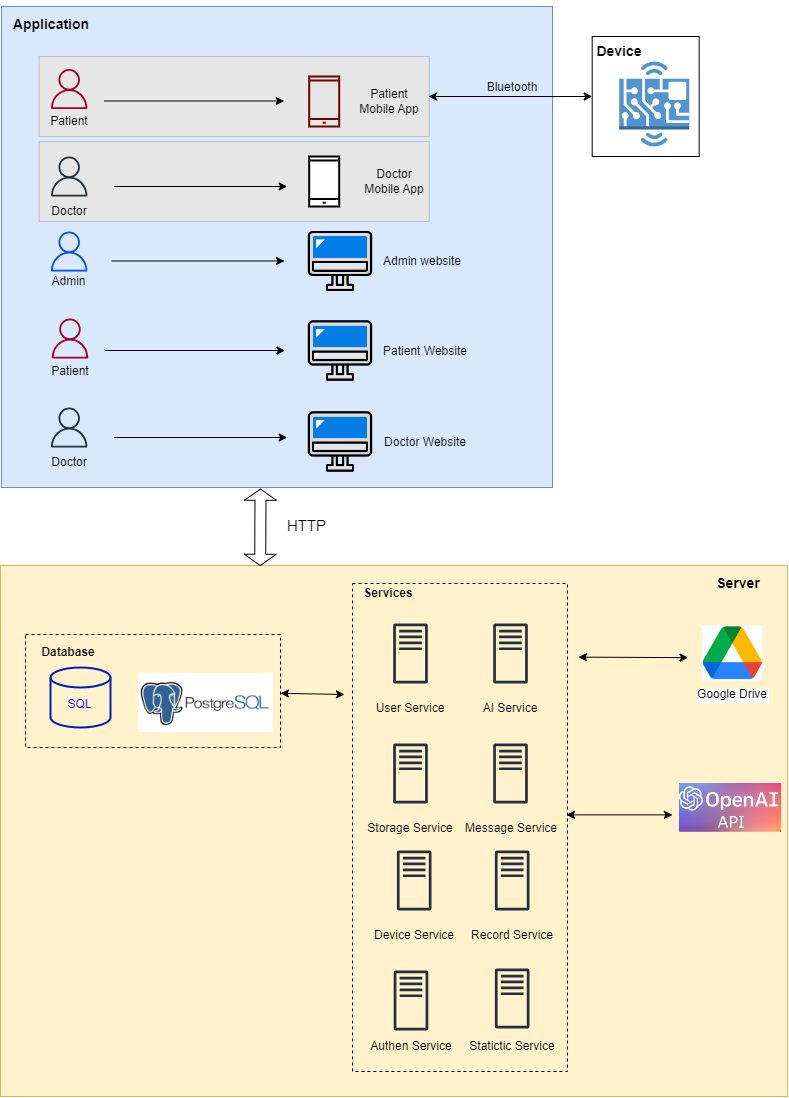
\includegraphics[width=12cm,height=12cm]{Images/system/fmECG_architecture-System_Architecture.png}
  \caption[Kiến trúc tổng quan hệ thống]{\bfseries \fontsize{12pt}{0pt}\selectfont Kiến trúc tổng quan hệ thống}
  \label{fmECG_architecture-System} %đặt tên cho ảnh
\end{figure}

Hình \ref{fmECG_architecture-System} thể hiện ba phần: 

\begin{adjustwidth}{1.5em}{}
\begin{itemize}
  \item Device: Thiết bị phần cứng đo điện tim, để kết nối với App bệnh nhân thông qua Bluetooth 
  \item Application: Bao gồm mobile app của bệnh nhân, bác sĩ và Website của Admin, Website của bác sĩ, Website của bệnh nhân
  \item Server: Bao gồm các Services để xử lý các yêu cầu gửi từ Application, cơ sở dữ liệu, Cloud lưu trữ, kết nối với model GPT-4 trên OpenAI thông qua api
\end{itemize}
\end{adjustwidth}

Trong hệ thống thì Devices và Mobile App là phần mà chúng em sẽ không trực tiếp thực hiện trong đồ án này, Website và Server sẽ là
phần mà đồ án chúng em thực hiện. Ở trong sơ đồ kiến trúc hệ thống riêng có bệnh nhân sẽ có tương tác trực tiếp với Devices,
còn lại khối Application sẽ tương tác với Server thông qua API với giao thức HTTP. Khi nhận được yêu cầu từ Application,
Server sẽ thực hiện xử lý dữ liệu, mọi yêu cầu đến đều được xử lý bởi các Services, tuỳ vào yêu cầu đến Services tương ứng sẽ đảm nhiệm 
việc lấy/lưu dữ liệu trong cơ sở dữ liệu sau đó trả ra kết quả cho người dùng.
\begin{adjustwidth}{1.5em}{}
\begin{itemize}
  \item User Services: Xử lý các yêu cầu liên quan đến người dùng như đăng ký, đăng nhập, lấy thông tin cá nhân
  \item Storage Services: Xử lý các tác vụ liên quan tới lưu trữ dữ liệu của hệ thống
  \item AI Services: Xử lý các tác vụ liên quan tới trợ lý ảo, bao gồm: huấn luyện, kết nối với model gpt-4 thông qua api và xử lý kết quả 
  và trả về tin nhắn và các hành động của ai can thiệp trực tiếp vào hệ thống 
  \item Message Services: Xử lý các yêu cầu liên quan tới hội thoại, tin nhắn.
  \item Device Services: Xử lý các tác vụ liên quan tới thiết bị như thêm, sửa, xoá thiết bị, cập nhật thông tin.
  \item Record Services: Xử lý các tác vụ liên quan tới bản ghi như là thêm sửa xoá, xử lý dữ liệu file đo, vẽ đồ thị
  \item Authen Services: Xử lý các tác vụ liên quan tới bảo mật như: mã hoá và cung cấp token, kiểm tra token, phân quyền truy cập api, mã hoá các dữ liệu nhạy cảm trước khi lưu trữ.
  \item Static Services: Xử lý các tác vụ liên quan tới thống kê như: thống kê người dùng, thiết bị, bản ghi, tin nhắn theo tuần theo tháng.
\end{itemize}
\end{adjustwidth}
Ngoài ra hệ thống sẽ có thêm chức năng tự động triển khai trên môi trường internet để việc phát triển và kiểm thử dễ dàng 
làm tăng chất lượng và độ hoàn thiện của hệ thống
Trên đây là tổng quan về kiến trúc hệ thống, phần tiếp dưới đây chúng em xin phép trình bày kỹ hơn về từng khối nhỏ hơn
dựa vào những đối tượng đã được xác định trong hệ thống.

\newpage
\subsection{Sơ đồ khối phần mềm}

\subsubsection{Website dành cho bệnh nhân}
\mbox{}

\begin{figure}[H]
  \centering
  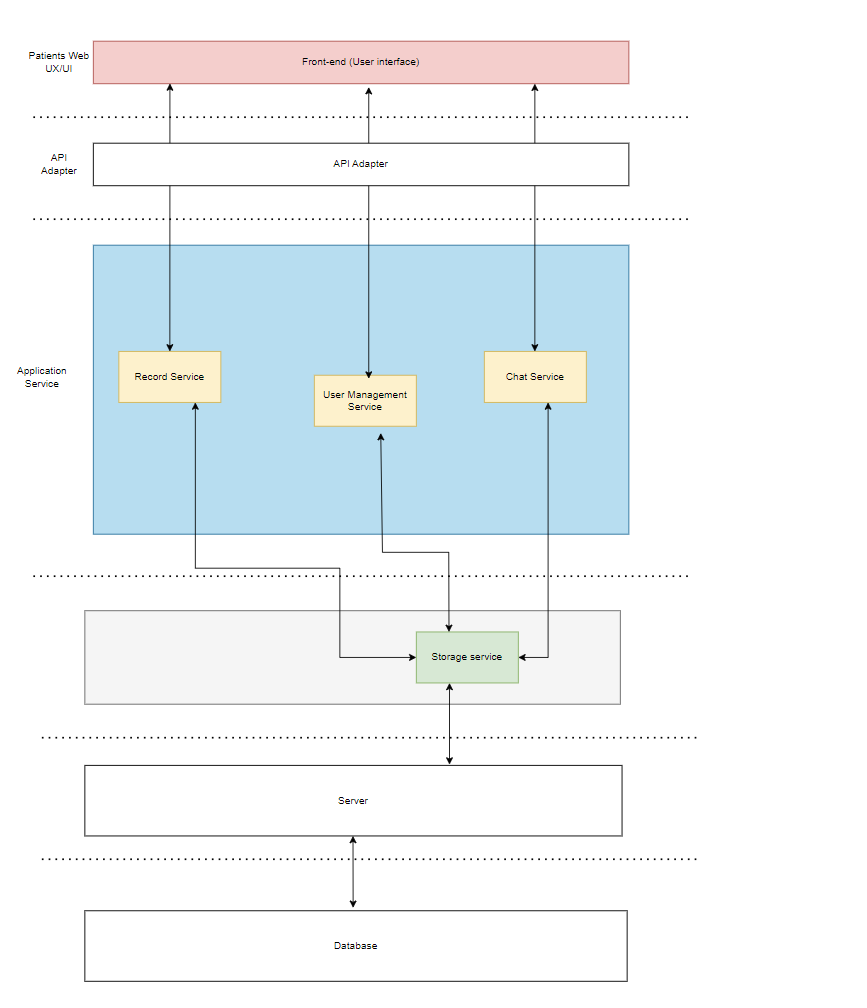
\includegraphics[width=12cm,height=14cm]{Images/system/fmECG_architecture-Patient.drawio.png}
  \caption[Sơ đồ khối cho App bệnh nhân]{\bfseries \fontsize{12pt}{0pt}\selectfont Sơ đồ khối cho App bệnh nhân}
  \label{fmECG_architecture-Patient} %đặt tên cho ảnh
\end{figure}

Trong hình trên, lớp trên cùng User interface là lớp để người dùng tương tác và thực hiện lời gọi thông qua API Adapter, 
các yêu cầu của người dùng sẽ được xử lý thông qua Services và phản hồi lại với người dùng qua giao diện. Dưới đây là phần
giải thích Services trong hình:
\begin{adjustwidth}{1.5em}{}
\begin{itemize}
  \item Record Service: Khối có nhiệm vụ xử lý yêu cầu cho chức năng đo và quản lý bản ghi: thực hiện đo, kết thúc đo, lưu kết quả đo, xử lý kết quả đo và cung cấp dữ liệu để vẽ đồ thị điện tim
  \item User Management Service: Khối có nhiệm vụ xử lý các vấn đề liên quan đến người dùng như đăng nhập, đăng ký, xem thông tin người dùng
  \item Device Service: Khối có nhiệm vụ xử lý các vấn đề liên quan đến thiết bị như thêm sửa xoá, thay đổi thông tin, cung cấp thiết bị cho người dùng
  \item Chat Service: Khối có nhiệm vụ quản lý việc chat, trao đổi thông tin với bác sĩ và trợ lý ảo
  \item Storage Service: Khối có nhiệm vụ lưu thông tin vào bộ nhớ
\end{itemize}
\end{adjustwidth}


\subsubsection{Website dành cho bác sĩ}

\begin{figure}[H]
  \centering
  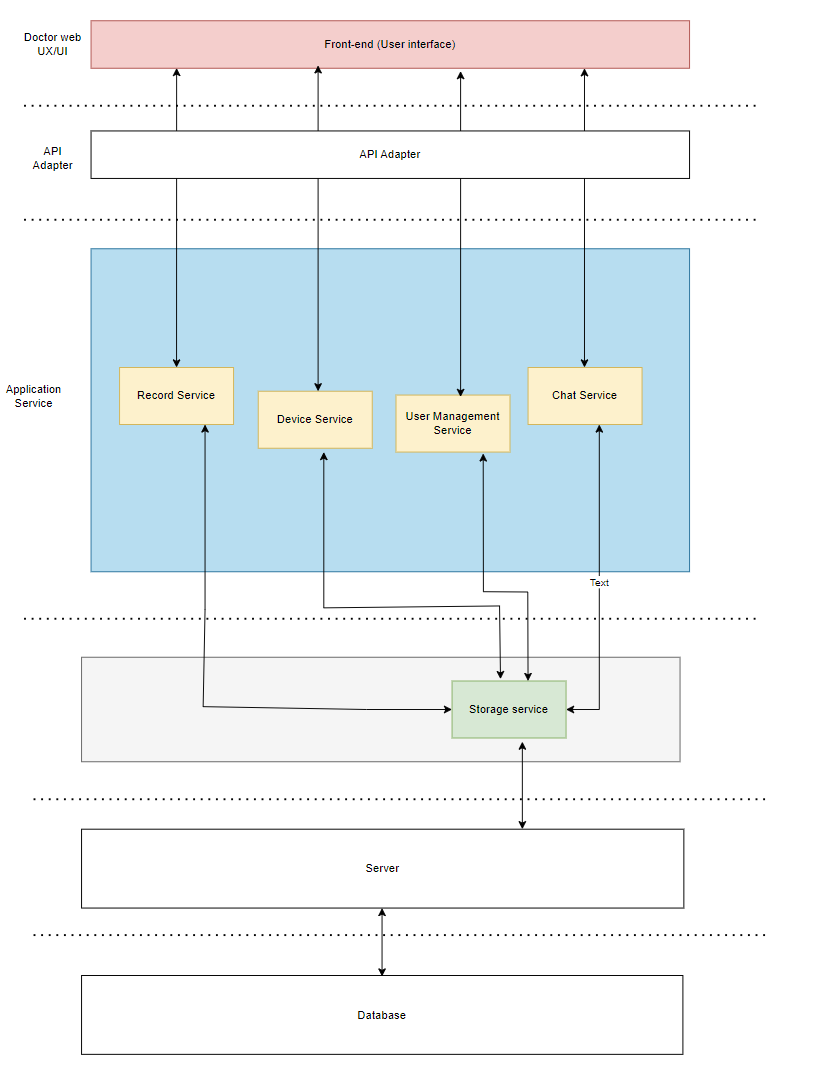
\includegraphics[width=12cm,height=14cm]{Images/system/fmECG_architecture-Doctors.drawio.png}
  \caption[Sơ đồ khói cho App bác sĩ]{\bfseries \fontsize{12pt}{0pt}\selectfont Sơ đồ khối cho App bác sĩ}
  \label{fmECG_architecture-Doctors} %đặt tên cho ảnh
\end{figure}

Về cơ bản, website cho bác sĩ có những khối tương tự với bệnh nhân, trừ việc bác sĩ sẽ có thêm quyền quản lý thiết bị (Device Service)

\subsubsection{Website cho quản trị viên}

\begin{figure}[H]
  \centering
  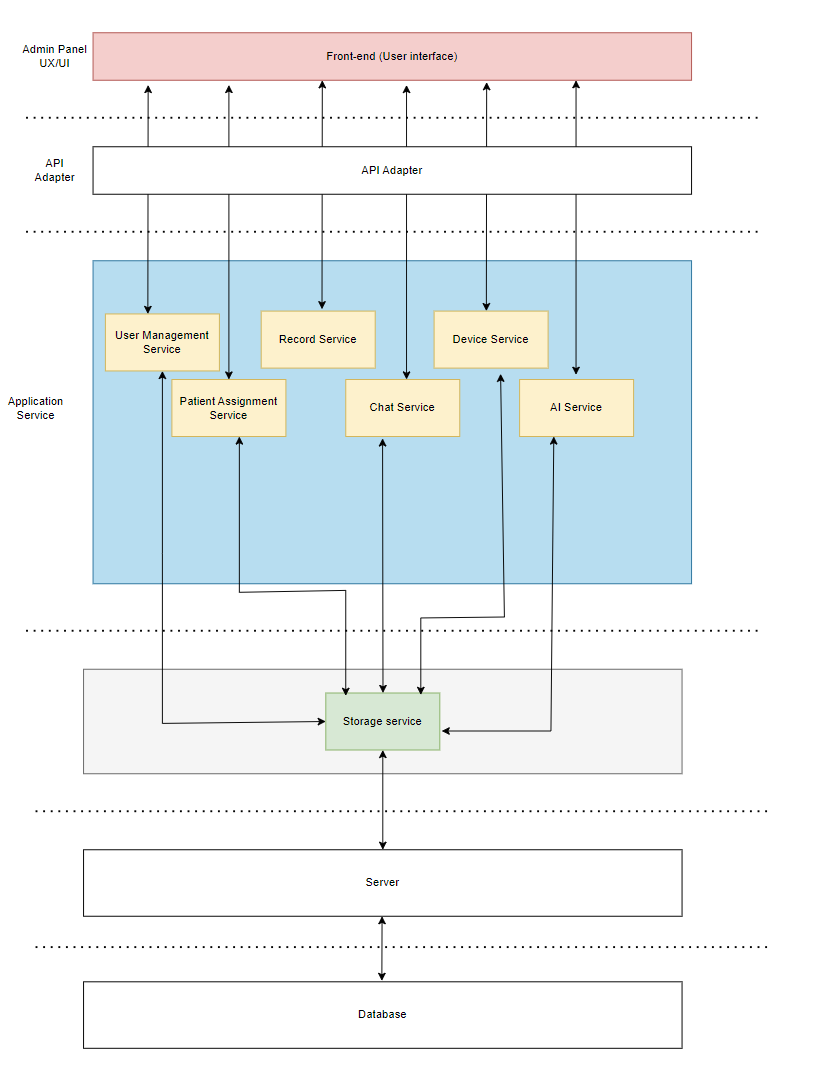
\includegraphics[width=12cm,height=14cm]{Images/system/fmECG_architecture-Admin.drawio.png}
  \caption[Sơ đồ khối cho Website quản trị viên]{\bfseries \fontsize{12pt}{0pt}\selectfont Sơ đồ khối cho Website quản trị viên}
  \label{fmECG_architecture-Admin} %đặt tên cho ảnh
\end{figure}

Quản trị viên sẽ quản lý 6 Services chính đó là quản lý người dùng (User Management Service), quản lý phân công
bác sĩ - bệnh nhân (Patient Assignment Service), quản lý bản ghi (Record Service), Chat Service, Thêm dữ liệu mới để huấn luyện trợ lý ảo (AI service).

Tiếp theo để phân tích cụ thể hơn từng luồng trong hệ thống qua use case, chúng em xin phép được trình bày các sơ đồ tuần
tự. 
\newpage

\subsection{Thiết kế cơ sở dữ liệu}
\label{design_database}

\subsubsection{Từ điển dữ liệu}

\begin{table}[H]
  \caption{\bfseries \fontsize{12pt}{0pt}\selectfont Bảng user}
  \centering
  \begin{tabularx}{0.9\textwidth}{|c|c|X|}
    \hline
    \textbf{Thuộc tính} & \textbf{Kiểu dữ liệu} & \textbf{Mô tả} \\
    \hline
    user\_id & STRING & Khóa chính của bảng, đại diện cho ID người dùng. \\
    \hline
    password & STRING & Mật khẩu của người dùng. \\
    \hline
    email & STRING & Địa chỉ email của người dùng. \\
    \hline
    name & STRING & Tên của người dùng. \\
    \hline
    gender & INT & Giới tính của người dùng. \\
    \hline
    birth & DATE & Ngày sinh của người dùng. \\
    \hline
    phone\_number & STRING & Số điện thoại của người dùng. \\
    \hline
    image & STRING & Ảnh đại diện của người dùng. \\
    \hline
    status & INTEGER & Trạng thái sử dụng của người dùng (0 - còn đang sử dụng, 1 - không còn đang sử dụng). \\
    \hline
    information & STRING & Thông tin thêm về người dùng. \\
    \hline
    role & INTEGER & Quyền của người dùng (0 - bệnh nhân, 1 - bác sĩ, 2 - quản trị viên). \\
    \hline
    created\_at & DATE & Thời điểm thêm mới dữ liệu vào CSDL. \\
    \hline
    updated\_at & DATE & Thời điểm cập nhật dữ liệu vào CSDL. \\
    \hline
    
  \end{tabularx}
\end{table}


\begin{table}[H]
  \caption{\bfseries \fontsize{12pt}{0pt}\selectfont Bảng account}
  \centering
  \begin{tabularx}{0.9\textwidth}{|c|c|X|}
    \hline
    \textbf{Thuộc tính} & \textbf{Kiểu dữ liệu} & \textbf{Mô tả} \\
    \hline
    account\_id & STRING & Khóa chính của bảng, đại diện cho ID tài khoản. \\
    \hline
    email & STRING & Địa chỉ email đăng kí của người dùng. \\
    \hline
    password & STRING & Mật khẩu của người dùng. \\
    \hline
  \end{tabularx}
\end{table}

\begin{table}[H]
  \caption{\bfseries \fontsize{12pt}{0pt}\selectfont Bảng register}
  \centering
  \begin{tabularx}{0.9\textwidth}{|c|c|X|}
    \hline
    \textbf{Thuộc tính} & \textbf{Kiểu dữ liệu} & \textbf{Mô tả} \\
    \hline
    register\_id & STRING & Khóa chính của bảng, đại diện cho ID tài khoản. \\
    \hline
    email & STRING & Địa chỉ email đăng kí của người dùng. \\
    \hline
    password & STRING & Mật khẩu của người dùng. \\
    \hline
    username & STRING & Tên của người dùng. \\
    \hline
    gender & INT & Giới tính của người dùng. \\
    \hline
    birth & DATE & Ngày sinh của người dùng. \\
    \hline
    phone\_number & STRING & Số điện thoại của người dùng. \\
    \hline
    image & STRING & Ảnh đại diện của người dùng. \\
    \hline
    status & INTEGER & Trạng thái chờ của người dùng (0 - đang chờ xử lý, 1 - được admin chấp nhận, 2 - bị admin từ chối). \\
    \hline
    information & STRING & Thông tin thêm về người dùng. \\
    \hline
    role & INTEGER & Quyền của người dùng (0 - bệnh nhân, 1 - bác sĩ, 2 - quản trị viên).\\
    \hline
  \end{tabularx}
\end{table}

\begin{table}[H]
  \caption{\bfseries \fontsize{12pt}{0pt}\selectfont Bảng record}
  \centering
  \begin{tabularx}{0.9\textwidth}{|c|c|X|}
    \hline
    \textbf{Thuộc tính} & \textbf{Kiểu dữ liệu} & \textbf{Mô tả} \\
    \hline
    record\_id & STRING & Khóa chính của bảng, đại diện cho ID bản ghi record. \\
    \hline
    user\_id & STRING & Khóa ngoại tham chiếu đến \texttt{user\_id} trong bảng \texttt{user}. \\
    \hline
    device\_id & STRING & Khóa ngoại tham chiếu đến \texttt{device\_id} trong bảng \texttt{device}, đại diện cho ID thiết bị. \\
    \hline
    record\_type & INTEGER & Loại của record (0 - PPG, 1 - PCG, 2 - HeartRate, 3 - ECG). \\
    \hline
    data\_directory & STRING & Đường dẫn lưu trữ dữ liệu. \\
    \hline
    start\_time & DATE & Thời gian bắt đầu ghi lại record. \\
    \hline
    stop\_time & DATE & Thời gian kết thúc ghi lại record. \\
    \hline
    sensor\_type & STRING & Loại cảm biến. \\
    \hline
    created\_at & DATE & Thời điểm thêm mới dữ liệu vào CSDL. \\
    \hline
    updated\_at & DATE & Thời điểm cập nhật dữ liệu vào CSDL. \\
    \hline
  \end{tabularx}
\end{table}

\begin{table}[H]
  \caption{\bfseries \fontsize{12pt}{0pt}\selectfont Bảng news\_category}
  \centering
  \begin{tabularx}{0.9\textwidth}{|c|c|X|}
    \hline
    \textbf{Thuộc tính} & \textbf{Kiểu dữ liệu} & \textbf{Mô tả} \\
    \hline
    category\_id & STRING & Khóa chính của bảng, đại diện cho ID danh mục tin tức. \\
    \hline
    category\_name & STRING & Tên danh mục tin tức. \\
    \hline
    category\_description & STRING & Mô tả danh mục tin tức. \\
    \hline
    created\_at & DATE & Thời điểm thêm mới dữ liệu vào CSDL. \\
    \hline
    updated\_at & DATE & Thời điểm cập nhật dữ liệu vào CSDL. \\
    \hline
  \end{tabularx}
\end{table}

\begin{table}[H]
  \caption{\bfseries \fontsize{12pt}{0pt}\selectfont Bảng news}
  \centering
  \begin{tabularx}{0.9\textwidth}{|c|c|X|}
    \hline
    \textbf{Thuộc tính} & \textbf{Kiểu dữ liệu} & \textbf{Mô tả} \\
    \hline
    news\_id & STRING & Khóa chính của bảng, đại diện cho ID tin tức. \\
    \hline
    title & STRING & Tiêu đề tin tức. \\
    \hline
    content & TEXT & Nội dung tin tức. \\
    \hline
    category\_id & INTEGER & Khóa ngoại tham chiếu đến \texttt{category\_id} trong bảng \texttt{news\_category}. \\
    \hline
    author & STRING & Tác giả tin tức. \\
    \hline
    url & STRING & Đường dẫn tin tức. \\
    \hline
    image & STRING & Đường dẫn hình ảnh tin tức (có thể là null). \\
    \hline
    created\_at & DATE & Thời điểm thêm mới dữ liệu vào CSDL. \\
    \hline
    updated\_at & DATE & Thời điểm cập nhật dữ liệu vào CSDL. \\
    \hline
  \end{tabularx}
\end{table}

\begin{table}[H]
  \caption{\bfseries \fontsize{12pt}{0pt}\selectfont Bảng patient\_doctor\_assignment}
  \centering
  \begin{tabularx}{0.9\textwidth}{|c|c|X|}
    \hline
    \textbf{Thuộc tính} & \textbf{Kiểu dữ liệu} & \textbf{Mô tả} \\
    \hline
    assign\_id & STRING & Khóa chính của bảng, đại diện cho ID phân công bệnh nhân - bác sĩ. \\
    \hline
    patient\_id & STRING & Khóa ngoại tham chiếu đến \texttt{user\_id} trong bảng \texttt{user} (với quyền là bệnh nhân). \\
    \hline
    doctor\_id & INTEGER & Khóa ngoại tham chiếu đến \texttt{user\_id} trong bảng \texttt{user} (với quyền là bác sĩ). \\
    \hline
    start\_date & DATE & Ngày bắt đầu phân công. \\
    \hline
    created\_at & DATE & Thời điểm thêm mới dữ liệu vào CSDL. \\
    \hline
    updated\_at & DATE & Thời điểm cập nhật dữ liệu vào CSDL. \\
    \hline
  \end{tabularx}
\end{table}

\begin{table}[H]
  \caption{\bfseries \fontsize{12pt}{0pt}\selectfont Bảng token}
  \centering
  \begin{tabularx}{0.9\textwidth}{|c|c|X|}
    \hline
    \textbf{Thuộc tính} & \textbf{Kiểu dữ liệu} & \textbf{Mô tả} \\
    \hline
    id & STRING & Khóa chính của bảng, đại diện cho ID mã thông báo đặt lại. \\
    \hline
    account\_id & STRING & Khóa ngoại tham chiếu đến \texttt{account\_id} trong bảng \texttt{account}. \\
    \hline
    access\_token & STRING & Mã đại diện cho người dùng thao tác với hệ thống. \\
    \hline
    refresh\_token & STRING & Mã đại diện cho người dùng thao tác với hệ thống sau khi \texttt{access\_token} hết hạn. \\
    \hline
    created\_at & DATE & Thời điểm thêm mới dữ liệu vào CSDL. \\
    \hline
    updated\_at & DATE & Thời điểm cập nhật dữ liệu vào CSDL. \\
    \hline
  \end{tabularx}
\end{table}




\begin{table}[H]
  \caption{\bfseries \fontsize{12pt}{0pt}\selectfont Bảng device}
  \centering
  \begin{tabularx}{0.9\textwidth}{|c|c|X|}
    \hline
    \textbf{Thuộc tính} & \textbf{Kiểu dữ liệu} & \textbf{Mô tả} \\
    \hline
    device\_id & STRING & Khóa chính của bảng, đại diện cho ID thiết bị. \\
    \hline
    user\_id & STRING & Khóa ngoại tham chiếu đến \texttt{user\_id} trong bảng \texttt{users}, đại diện cho ID bệnh nhân. \\
    \hline
    doctor\_id & STRING & Khóa ngoại tham chiếu đến \texttt{user\_id} trong bảng \texttt{users}, đại diện cho ID bác sĩ. \\
    \hline
    device\_name & STRING & Tên thiết bị. \\
    \hline
    information & STRING & Thông tin thêm về thiết bị. \\
    \hline
    device\_type & INTEGER & Loại thiết bị (1 - thiết bị đo điện tim, 2 - thiết bị đo nhịp tim, âm thanh tim). \\
    \hline
    start\_date & DATE & Thời điểm bắt đàu sử dụng thiết bị. \\
    \hline
    status & INTEGER & Trạng thái của thiết bị (0 - đang được sử dụng, 1 - đang không được sử dụng). \\
    \hline
    created\_at & DATE & Thời điểm thêm mới dữ liệu vào CSDL. \\
    \hline
    updated\_at & DATE & Thời điểm cập nhật dữ liệu vào CSDL. \\
    \hline
  \end{tabularx}
\end{table}


\begin{table}[H]
  \caption{\bfseries \fontsize{12pt}{0pt}\selectfont Bảng device\_detail}
  \centering
  \begin{tabularx}{0.9\textwidth}{|c|c|X|}
    \hline
    \textbf{Thuộc tính} & \textbf{Kiểu dữ liệu} & \textbf{Mô tả} \\
    \hline
    device\_detail\_id & STRING & Khóa chính của bảng, đại diện cho ID thông tin một device. \\
    \hline
    device\_id & STRING & Khóa ngoại tham chiếu đến \texttt{device\_id} trong bảng \texttt{device}. \\
    \hline
    detail\_name & STRING & Tên trường liên quan thiết bị dựa vào \texttt{detail\_type}. \\
    \hline
    infomation & STRING & Thông tin về trường \texttt{detail\_name} của thiết bị. \\
    \hline
    value & STRING & Giá trị về loại thông tin của thiết bị dựa vào \texttt{detail\_type} (1 - tần số, 2 - dữ liệu kết nối, 3 - dung lượng lưu trữ). \\
    \hline
    detail\_type & INTEGER & Loại thông tin về thiết bị (1 - tín hiệu đo, 2 - loại kết nối, 3 - kiểu lưu trữ). \\
    \hline
    created\_at & DATE & Thời điểm thêm mới dữ liệu vào CSDL. \\
    \hline
    updated\_at & DATE & Thời điểm cập nhật dữ liệu vào CSDL. \\
    \hline
  \end{tabularx}
\end{table}

\begin{table}[H]
  \caption{\bfseries \fontsize{12pt}{0pt}\selectfont Bảng conversation}
  \centering
  \begin{tabularx}{0.9\textwidth}{|c|c|X|}
    \hline
    \textbf{Thuộc tính} & \textbf{Kiểu dữ liệu} & \textbf{Mô tả} \\
    \hline
    conversation\_id & STRING & Khóa chính của bảng, đại diện cho ID hội thoại. \\
    \hline
    name & STRING & Tên cuộc hội thoại. \\
    \hline
    type & INTEGER & Loại của cuộc hội thoại (0 - hội thoại 2 người, 1 - hội thoại nhóm, 2 - chatbot). \\
    \hline
    avatar & STRING & Đoạn mã chứa url ảnh đại diện của cuộc hội thoại  \\
    \hline
    created\_at & DATE & Thời điểm thêm mới dữ liệu vào CSDL \\
    \hline
    updated\_at & DATE & Thời điểm cập nhật dữ liệu vào CSDL \\
    \hline
  \end{tabularx}
\end{table}

\begin{table}[H]
  \caption{\bfseries \fontsize{12pt}{0pt}\selectfont Bảng message}
  \centering
  \begin{tabularx}{0.9\textwidth}{|c|c|X|}
    \hline
    \textbf{Thuộc tính} & \textbf{Kiểu dữ liệu} & \textbf{Mô tả} \\
    \hline
    message\_id & STRING & Khóa chính của bảng, đại diện cho ID tin nhắn. \\
    \hline
    conversation\_id & STRING & Khóa ngoại tham chiếu đến \texttt{conversation\_id} trong bảng \texttt{conversation}, đại diện cho ID hội thoại chứa tin nhắn. \\
    \hline
    sender\_id & STRING & Khóa ngoại tham chiếu đến \texttt{id} trong bảng \texttt{conversation\_member}, đại diện cho ID người gửi tin nhắn. \\
    \hline
    attachments & LIST <Map> & Danh sách tệp tin đính kèm khi gửi tin nhắn.\\
    \hline
    system\_message & BOOLEAN & Tin nhắn trả về từ hệ thống.\\
    \hline
    pin & BOOLEAN & Đánh dấu tin nhắn có được ghim không.\\
    \hline
    pin\_time & DATE & Thời gian ghim tin nhắn.\\
    \hline
    reactions & LIST <Map> & Danh sách các phản ứng lại với tin nhắn này.\\
    \hline
    created\_at & DATE & Thời điểm thêm mới dữ liệu vào CSDL \\
    \hline
    updated\_at & DATE & Thời điểm cập nhật dữ liệu vào CSDL \\
    \hline
  \end{tabularx}
\end{table}

\begin{table}[H]
  \caption{\bfseries \fontsize{12pt}{0pt}\selectfont Bảng conversation\_member}
  \centering
  \begin{tabularx}{0.9\textwidth}{|c|c|X|}
    \hline
    \textbf{Thuộc tính} & \textbf{Kiểu dữ liệu} & \textbf{Mô tả} \\
    \hline
    id & STRING & Khóa chính của bảng, đại diện cho ID của thành viên đoạn hội thoại. \\
    \hline
    conversation\_id & STRING & Khóa ngoại tham chiếu đến \texttt{conversation\_id} trong bảng \texttt{conversation}, đại diện cho ID hội thoại chứa tin nhắn. \\
    \hline
    user\_id & STRING & Khóa ngoại tham chiếu đến \texttt{user\_id} trong bảng \texttt{user}, đại diện cho ID người gửi tin nhắn. \\
    \hline
    status\_notify & INTEGER & Trạng thái thông báo tin nhắn (0 - có thông báo tin nhắn, 1 - không nhận thông báo tin nhắn).\\
    \hline
    seen & BOOLEAN & Tin nhắn đã được xem chưa.\\
    \hline
    role & INTEGER & Vai trò của người dùng trong hội thoại (tương ứng trong bảng \texttt{user}).\\
    \hline
    created\_at & DATE & Thời điểm thêm mới dữ liệu vào CSDL \\
    \hline
    updated\_at & DATE & Thời điểm cập nhật dữ liệu vào CSDL \\
    \hline
  \end{tabularx}
\end{table}


\begin{table}[H]
  \caption{\bfseries \fontsize{12pt}{0pt}\selectfont Bảng conversation\_attachment}
  \centering
  \begin{tabularx}{0.9\textwidth}{|c|c|X|}
    \hline
    \textbf{Thuộc tính} & \textbf{Kiểu dữ liệu} & \textbf{Mô tả} \\
    \hline
    id & STRING & Khóa chính của bảng, đại diện cho ID tệp đính kèm tin nhắn. \\
    \hline
    conversation\_id & STRING & Khóa ngoại tham chiếu đến \texttt{conversation\_id} trong bảng \texttt{conversation}, đại diện cho ID hội thoại chứa tin nhắn. \\
    \hline
    message\_id & STRING & Khóa ngoại tham chiếu đến \texttt{message\_id} trong bảng \texttt{message}, đại diện cho ID tin nhắn. \\
    \hline
    content\_url & STRING & Đoạn mã chứa nội dung của tệp tin.\\
    \hline
    file\_name & STRING & Tên của tệp tin.\\
    \hline
    size & INTEGER & Dung lượng của tệp tin.\\
    \hline
    thumbnail\_url & STRING & Đoạn mã chứa hình ảnh tĩnh của tệp tin.\\
    \hline
    type & INTEGER & Loại của tệp tin (0 - ảnh, 1 - video, 2 - tệp). \\
    \hline
    created\_at & DATE & Thời điểm thêm mới dữ liệu vào CSDL \\
    \hline
    updated\_at & DATE & Thời điểm cập nhật dữ liệu vào CSDL \\
    \hline
  \end{tabularx}
\end{table}

\subsubsection{Sơ đồ ERD}

\begin{figure}[H]
  \centering
  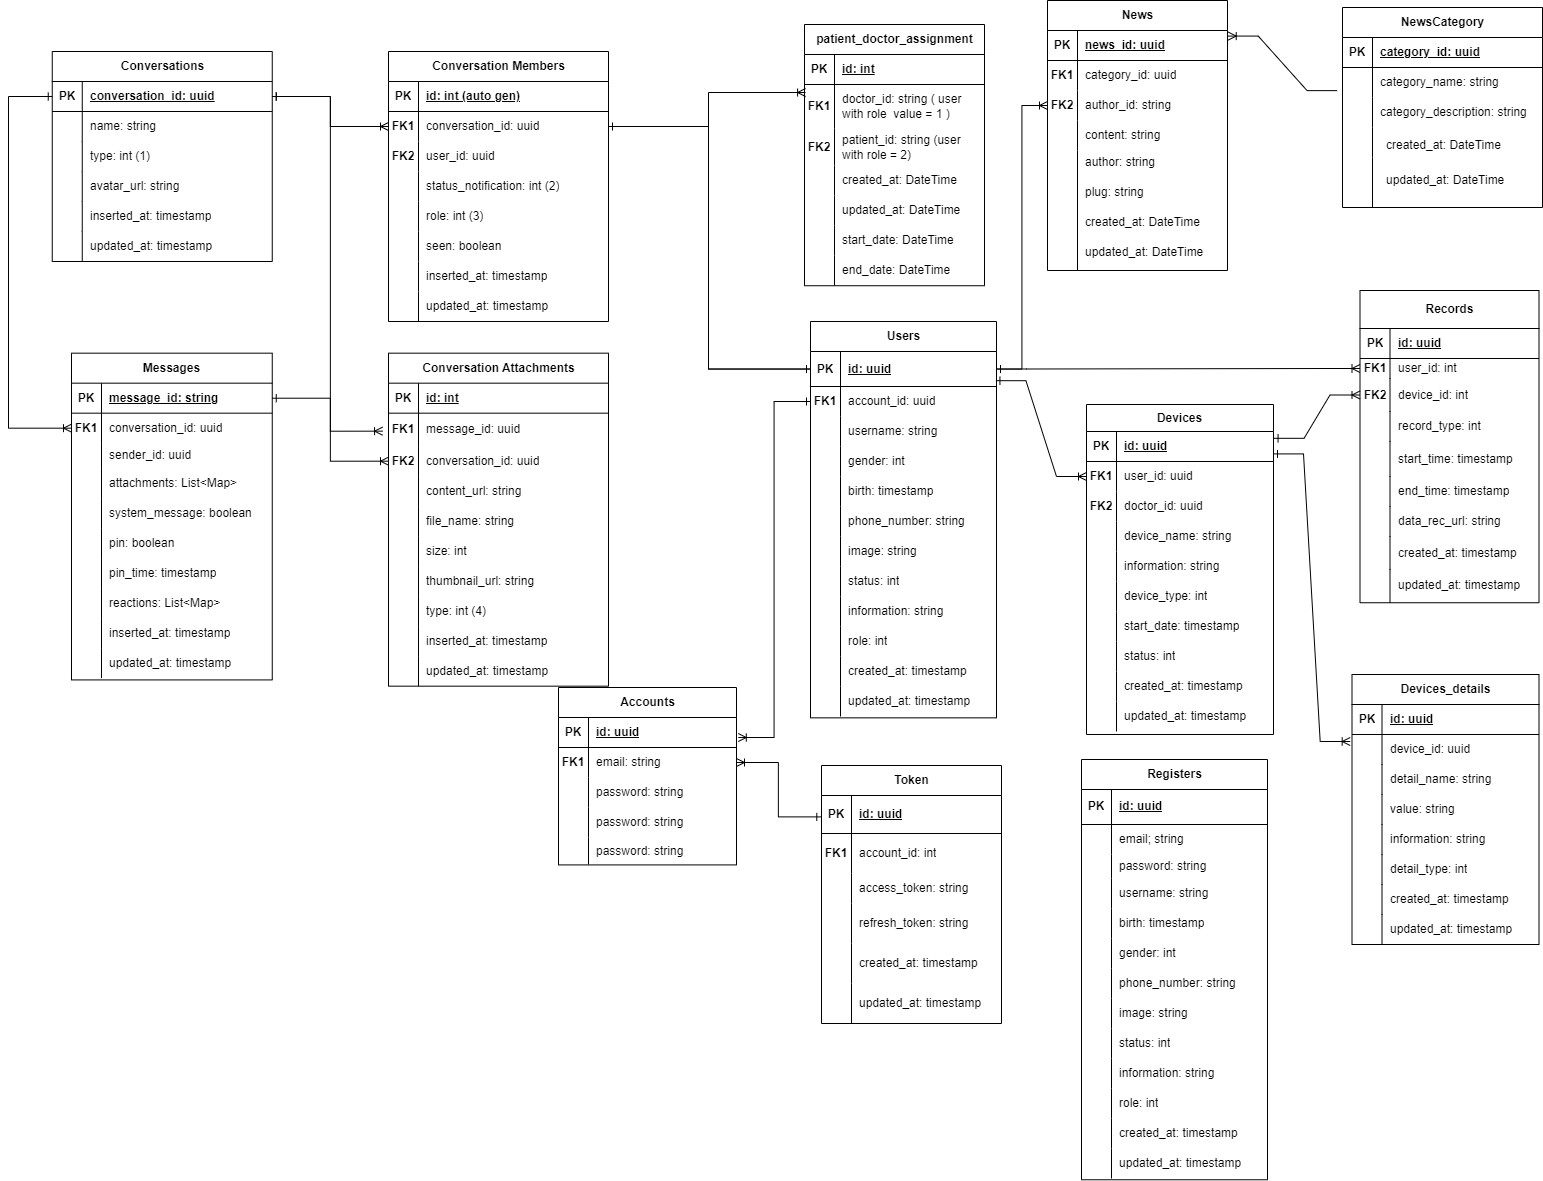
\includegraphics[width=15cm,height=15cm]{Images/system/fmECG_database.png}
  \caption[Sơ đồ ERD]{\bfseries \fontsize{12pt}{0pt}\selectfont Sơ đồ ERD}
  \label{fmECG_architecture-Database} %đặt tên cho ảnh
\end{figure}

\subsection{Thiết kế giao diện}

Dưới đây là các giao diện thực tế mà chúng em thiết kế cho trang web quản trị

\begin{figure}[H]
  \centering
  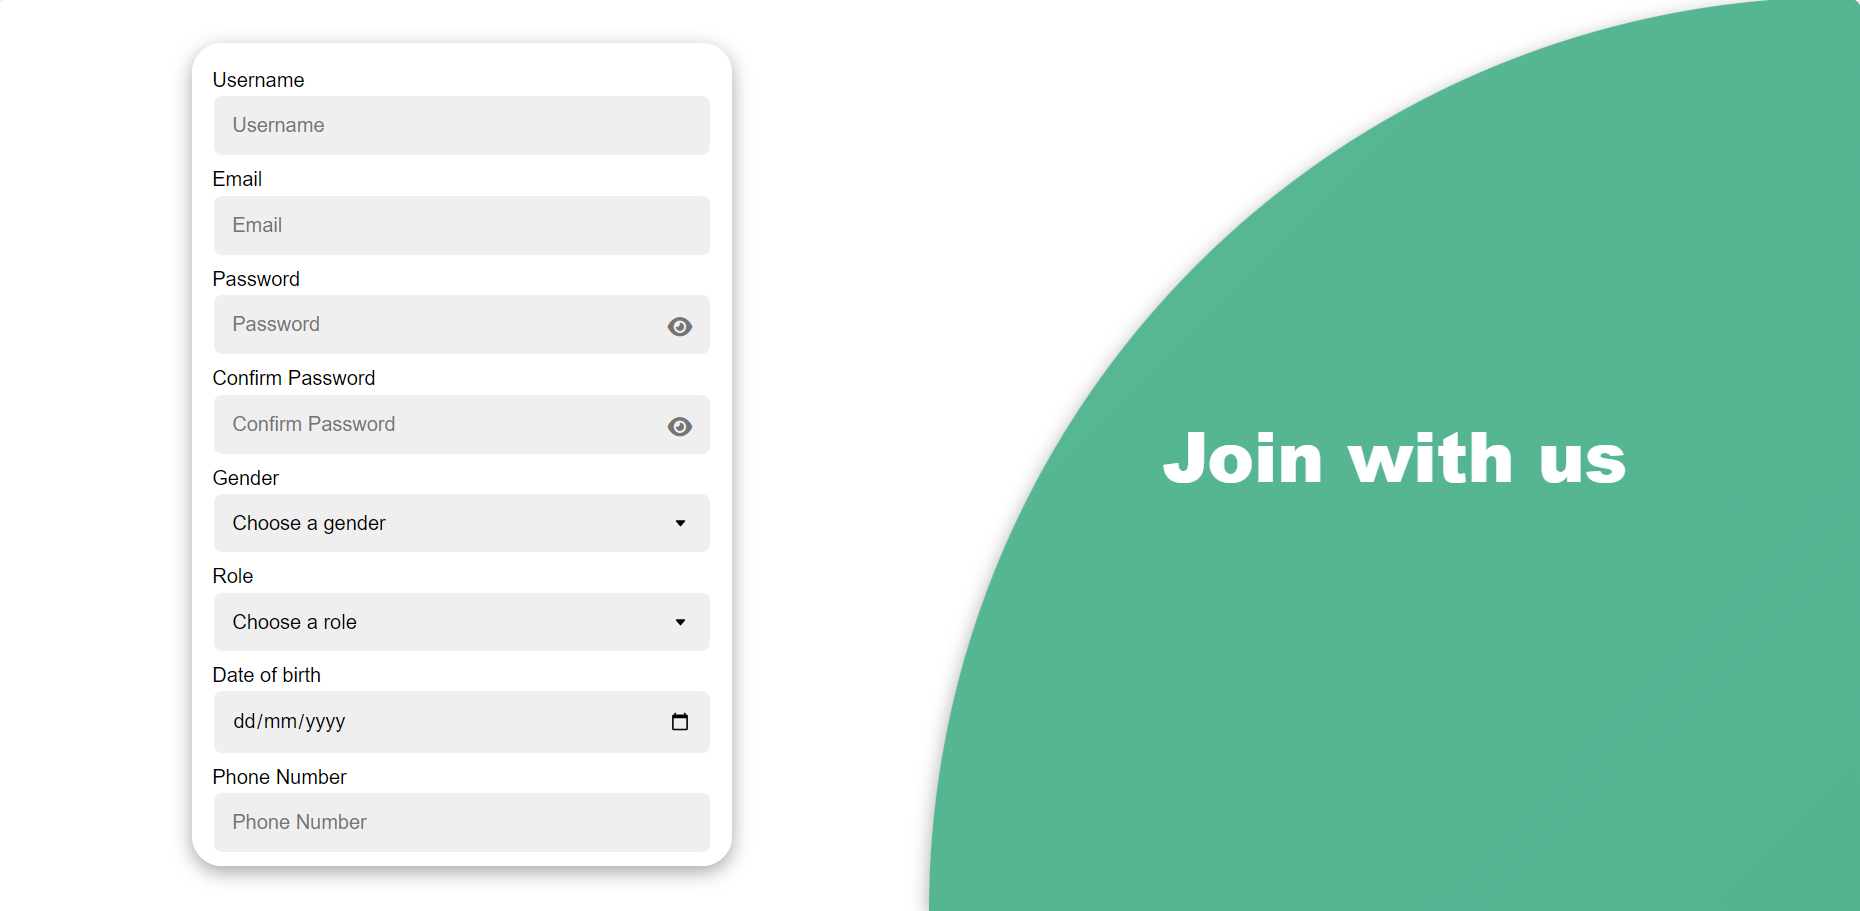
\includegraphics[scale=0.4]{Images/server/webUI/register_1.png}
  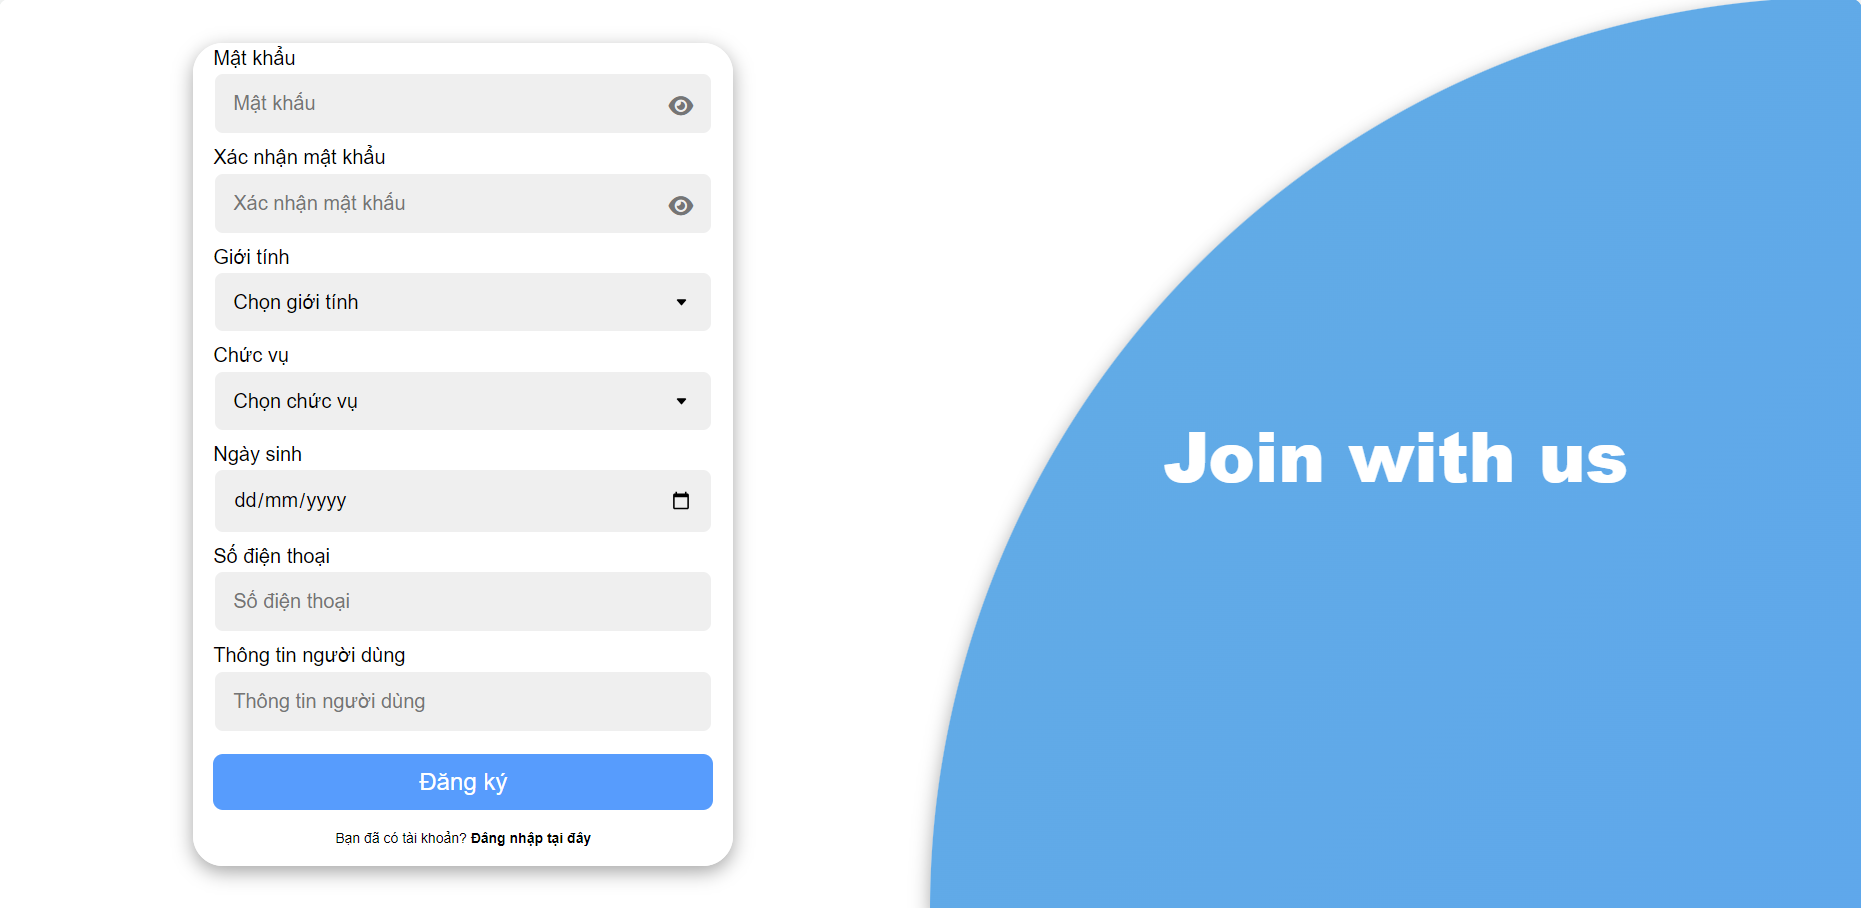
\includegraphics[scale=0.4]{Images/server/webUI/register_2.png}
  \caption[Giao diện trang đăng ký tài khoản]{\bfseries \fontsize{12pt}{0pt}\selectfont Giao diện trang đăng ký tài khoản}
  \label{register} %đặt tên cho ảnh
\end{figure}

Hình \ref{register} mô tả giao diện cho màn hình đăng ký tài khoản, màn hình này sẽ bao
 gồm các thông tin để người dùng đăng ký tài khoản vào hệ thống
 nếu các thông tin là chính xác thì sẽ chuyển hướng đến trang đăng nhập và chờ kết quả phê duyệt qua email, 
 còn nếu sai thông tin thì sẽ có popup thông báo sai trường thông tin

\begin{figure}[H]
  \centering
  \includegraphics[scale=0.4]{Images/server/webUI/login.png}
  \caption[Giao diện trang đăng nhập]{\bfseries \fontsize{12pt}{0pt}\selectfont Giao diện trang đăng nhập}
  \label{login} %đặt tên cho ảnh
\end{figure}

Hình \ref{login} mô tả giao diện cho màn hình đăng nhập, màn hình này sẽ bao
 gồm hai trường thông tin là Tên đăng nhập và Mật khẩu để người dùng đăng nhập vào trang quản trị
 nếu hai trường thông tin username và password là chính xác thì sẽ chuyển hướng đến trang dashboard 
 quản lý, còn nếu sai thông tin thì sẽ có popup thông báo sai tên đăng nhập hoặc mật khẩu hiện lên

 \begin{figure}[H]
  \centering
  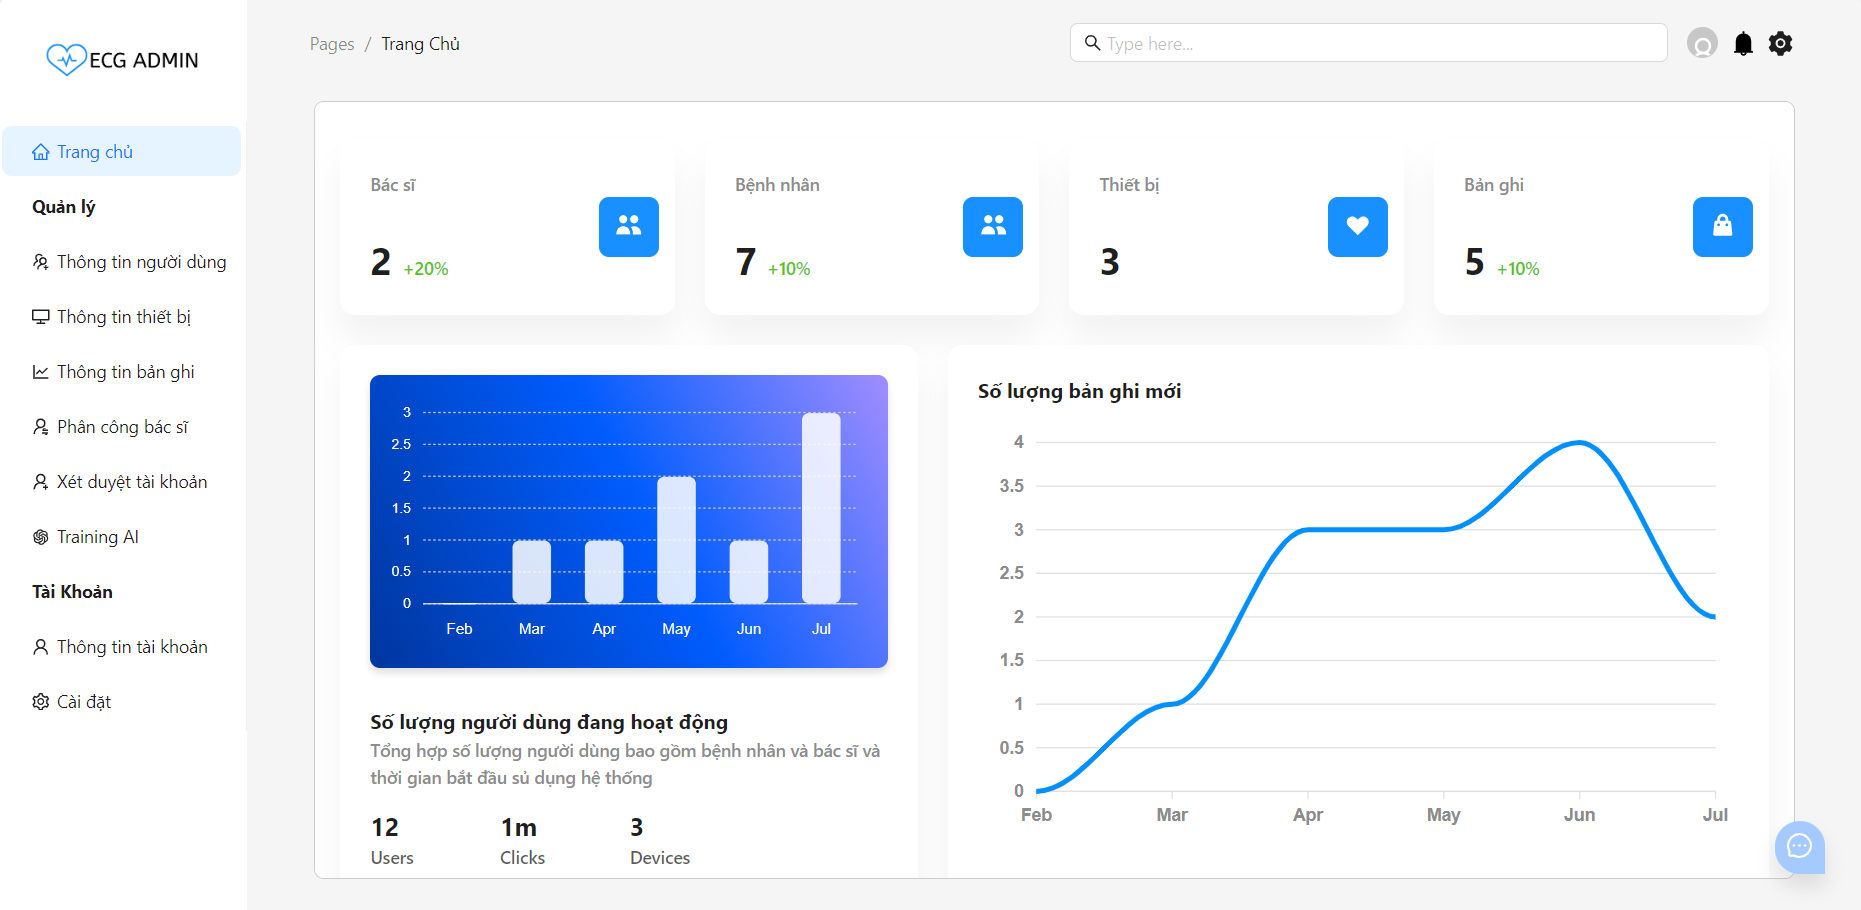
\includegraphics[scale=0.4]{Images/server/webUI/dashboard_admin.png}
  \caption[Giao diện trang dashboard dành cho admin sau khi đăng nhập thành công]{\bfseries \fontsize{12pt}{0pt}\selectfont Giao diện trang dashboard dành cho admin sau khi đăng nhập thành công}
  \label{dashboard_admin} %đặt tên cho ảnh
\end{figure}

\begin{figure}[H]
  \centering
  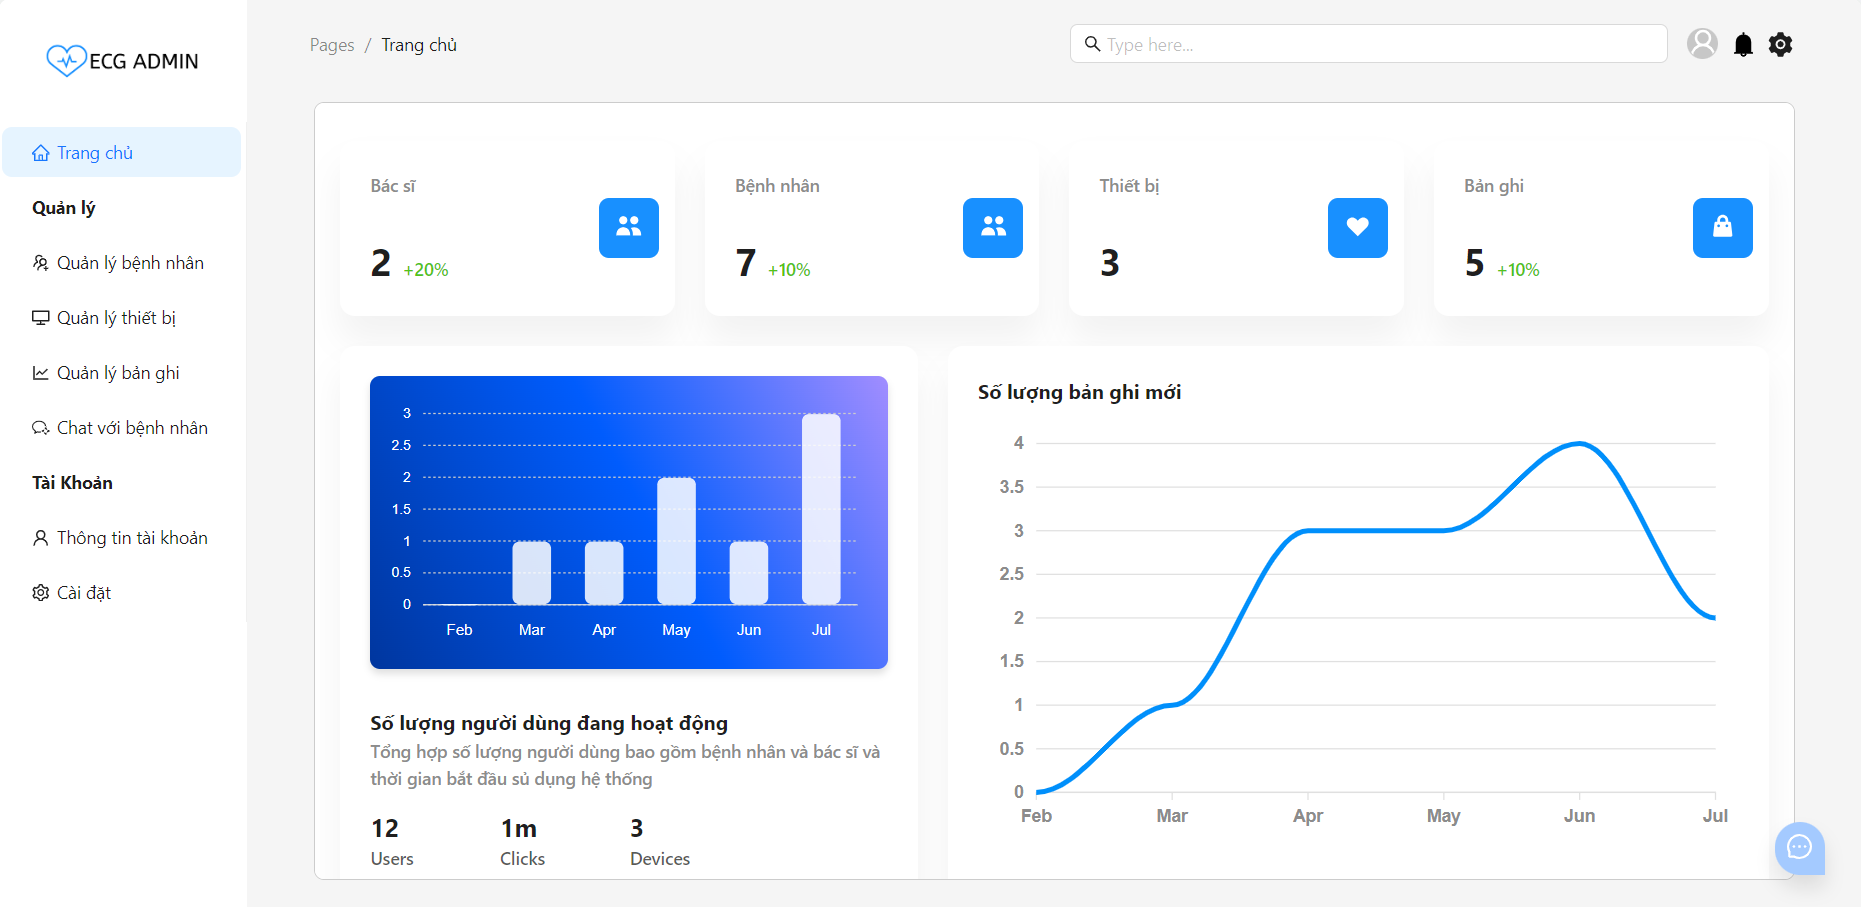
\includegraphics[scale=0.4]{Images/server/webUI/dashboard_doctor.png}
  \caption[Giao diện trang dashboard dành cho bác sĩ sau khi đăng nhập thành công]{\bfseries \fontsize{12pt}{0pt}\selectfont Giao diện trang dashboard dành cho bác sĩ sau khi đăng nhập thành công}
  \label{dashboard_doctor} %đặt tên cho ảnh
\end{figure}

\begin{figure}[H]
  \centering
  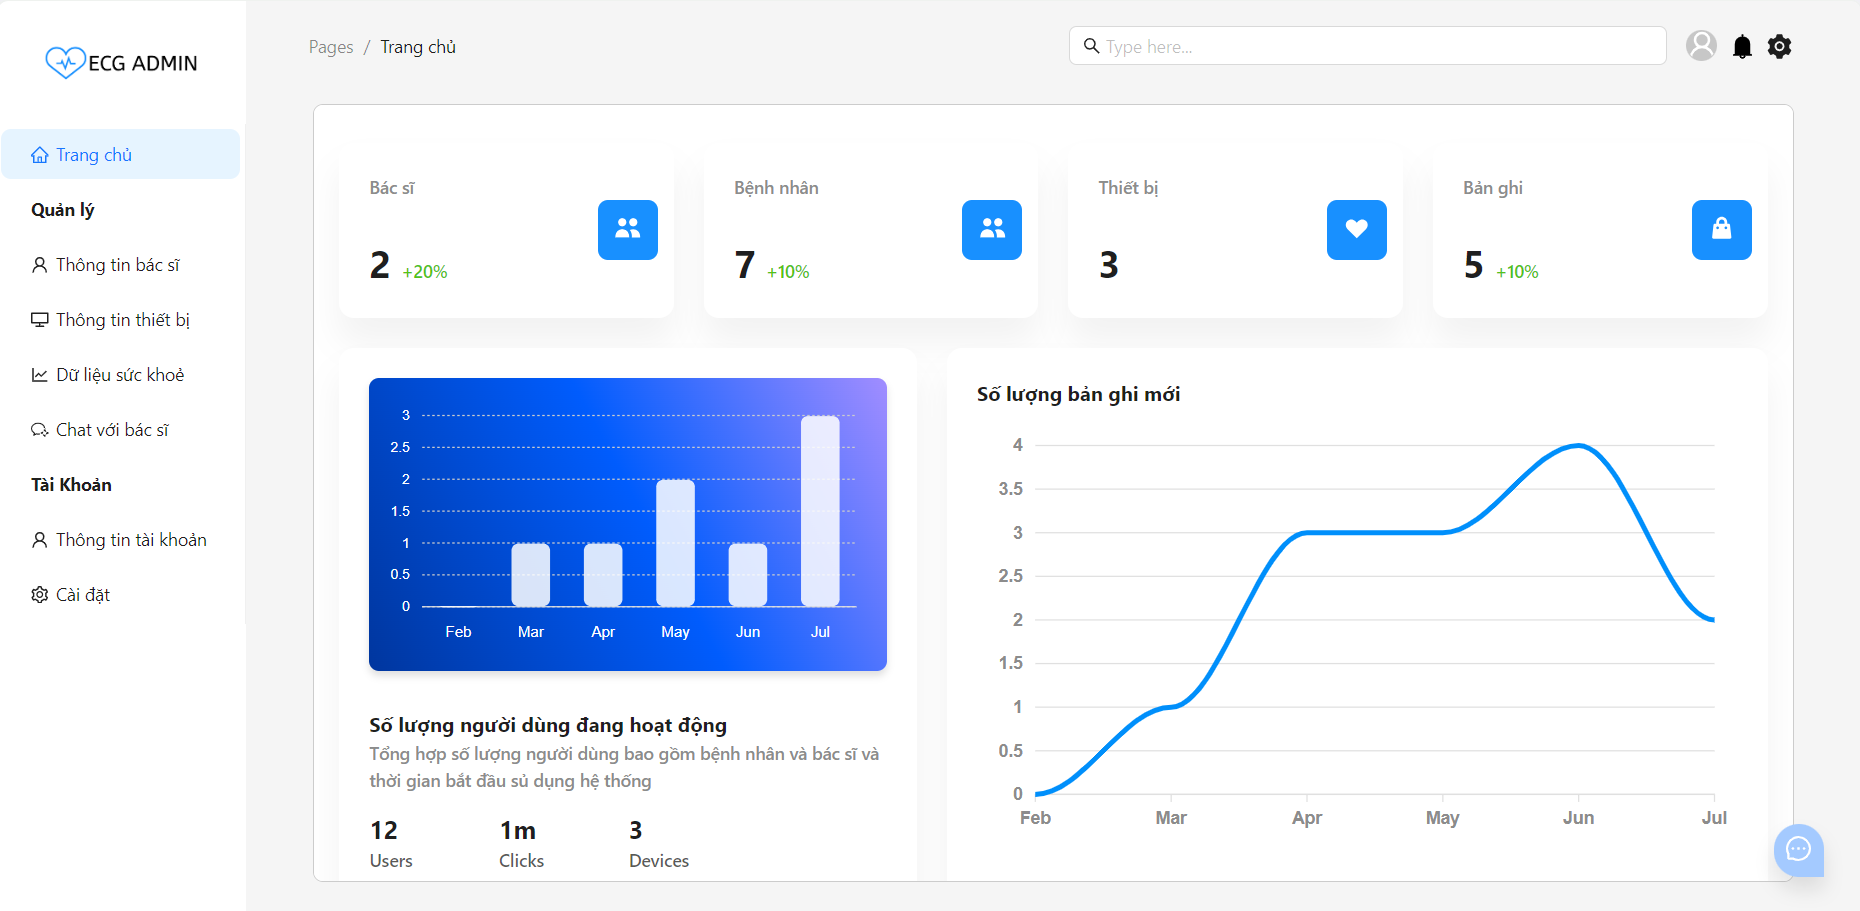
\includegraphics[scale=0.4]{Images/server/webUI/dashboard_patient.png}
  \caption[Giao diện trang dashboard dành cho bệnh nhân sau khi đăng nhập thành công]{\bfseries \fontsize{12pt}{0pt}\selectfont Giao diện trang dashboard dành cho bệnh nhân sau khi đăng nhập thành công}
  \label{dashboard_patient} %đặt tên cho ảnh
\end{figure}

Hình \ref{dashboard_admin}, \ref{dashboard_doctor}, \ref{dashboard_patient} mô tả giao diện cho trang dashboard, trong màn hình này phần bên trái sẽ bao
 gồm thanh điều hướng dẫn đến trang quản lý từng mục khác nhau theo từng loại tài khoản (admin, bác sĩ, bệnh nhân) và 
 thông tin tài khoản. Còn ở giữa là thông tin tổng số các mục mà hệ thống quản lý (người dùng, thiết bị, bản ghi)
 cùng với đó là biểu đồ thống kê số lượng người dùng và bản ghi mới theo tháng.

\begin{figure}[H]
  \centering
  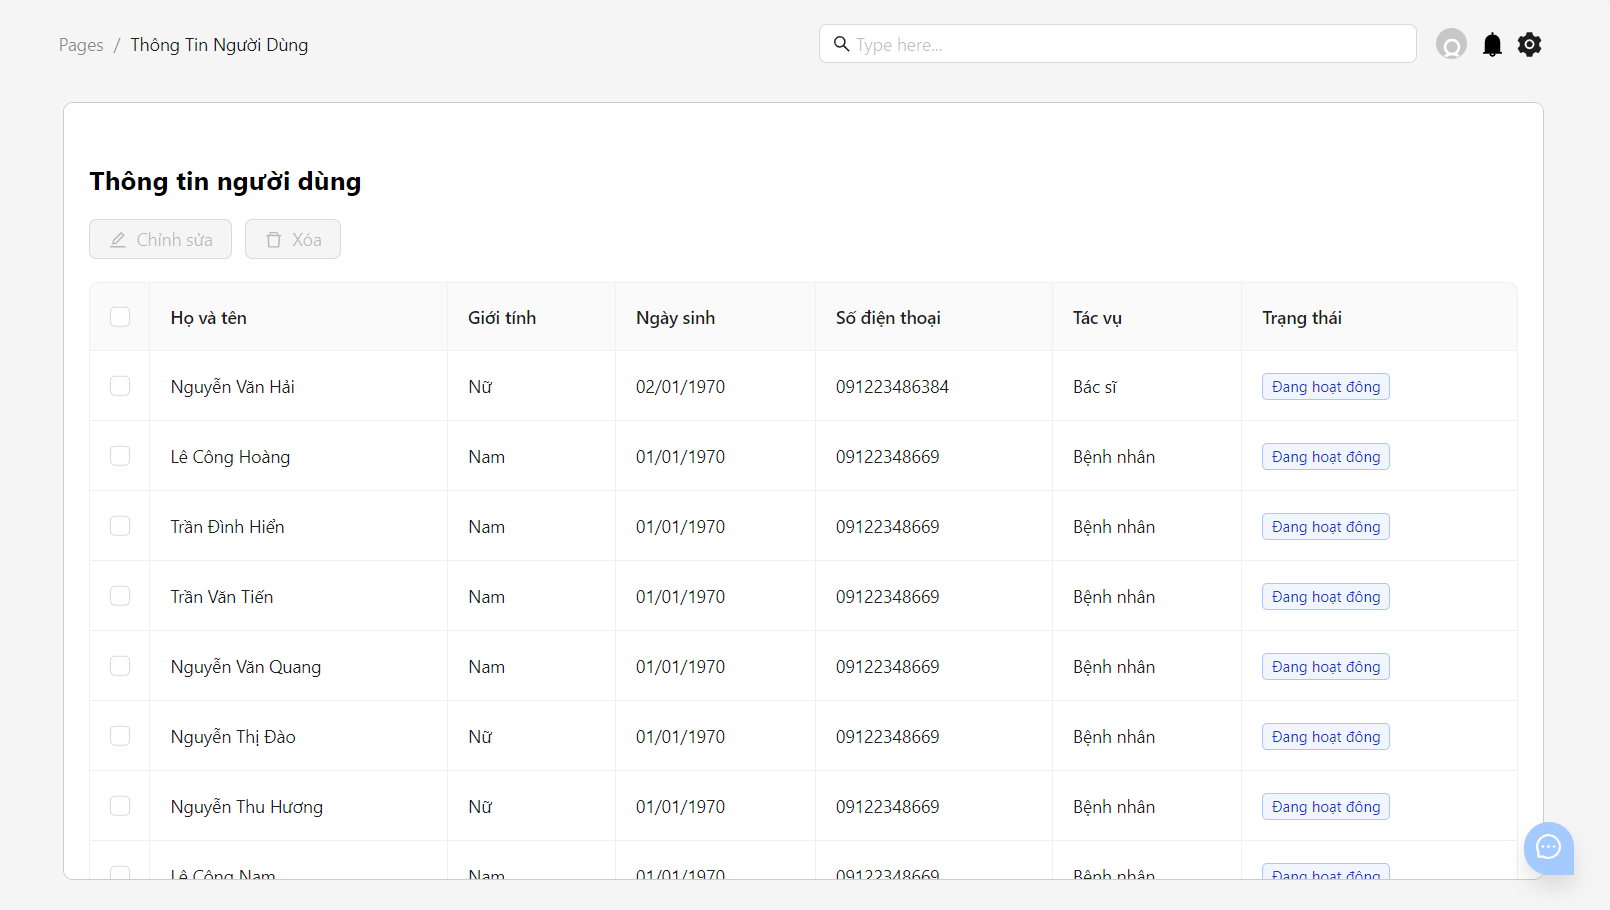
\includegraphics[scale=0.5]{Images/server/webUI/userTable.png}
  \caption[Giao diện trang quản lý người dùng]{\bfseries \fontsize{12pt}{0pt}\selectfont Giao diện trang quản lý người dùng}
  \label{userTable} %đặt tên cho ảnh
\end{figure}

Hình \ref{userTable} mô tả giao diện cho trang quản lý người dùng, trang này sẽ hiển thị danh sách
thông tin của các người dùng đang có trên hệ thống, bên cạnh đó khi tích vào mỗi bệnh
nhân tương ứng sẽ có các lựa chọn để xem chi tiết thông tin người dùng, cập nhật thông
tin hay xóa thông tin.

\begin{figure}[H]
  \centering
  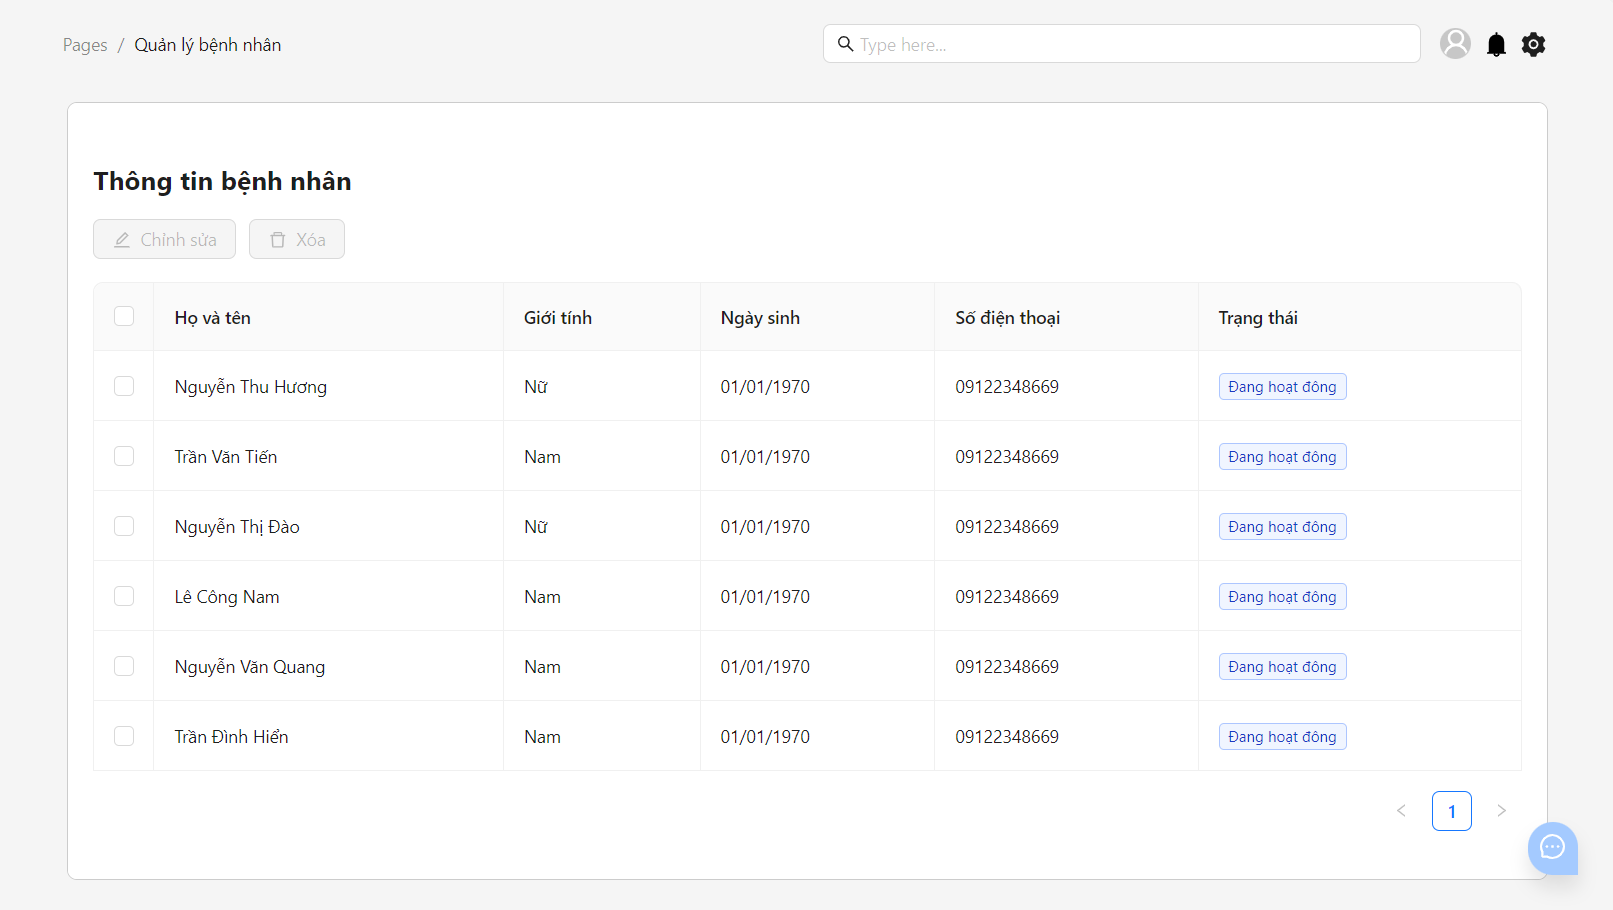
\includegraphics[scale=0.5]{Images/server/webUI/patientTable.png}
  \caption[Giao diện trang quản lý bệnh nhân]{\bfseries \fontsize{12pt}{0pt}\selectfont Giao diện trang quản lý bệnh nhân}
  \label{patientTable} %đặt tên cho ảnh
\end{figure}

Hình \ref{patientTable} mô tả giao diện cho trang quản lý bệnh nhân, trang này có giao diện tương tự với trang 
quản lý người dùng ở hình \ref{userTable} nhưng thông tin ở đây sẽ dành cho bác sĩ, và trang này chỉ có chức năng xem thông tin bệnh nhân.

\begin{figure}[H]
  \centering
  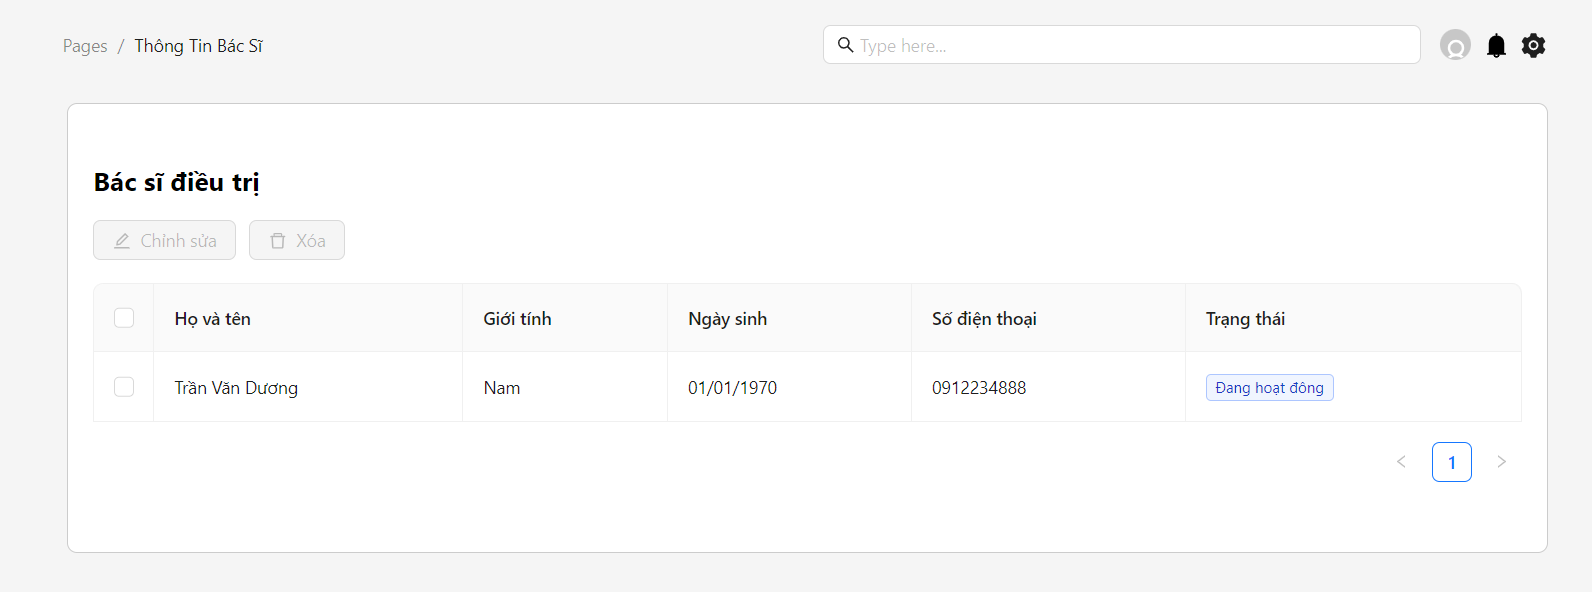
\includegraphics[scale=0.5]{Images/server/webUI/manageDoctor.png}
  \caption[Giao diện trang danh sách bác sĩ phụ trách]{\bfseries \fontsize{12pt}{0pt}\selectfont Giao diện trang danh sách bác sĩ phụ trách}
  \label{doctorTable} %đặt tên cho ảnh
\end{figure}

Hình \ref{doctorTable} mô tả giao diện cho trang danh sách bác sĩ phụ trách, trang này có giao diện tương tự với trang 
quản lý người dùng ở hình \ref{userTable} nhưng thông tin ở đây sẽ dành cho bệnh nhân, và trang này chỉ có chức năng xem thông tin bác sĩ.

\begin{figure}[H]
  \centering
  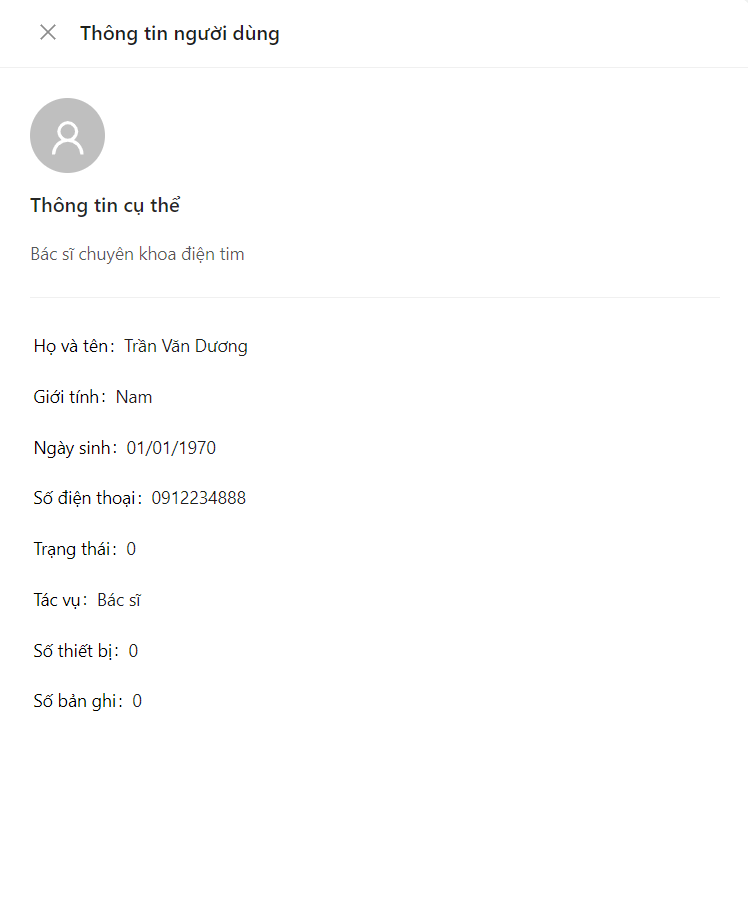
\includegraphics[scale=0.7]{Images/server/webUI/userInfo.png}
  \caption[Giao diện màn thông tin chi tiết người dùng]{\bfseries \fontsize{12pt}{0pt}\selectfont Giao diện màn thông tin chi tiết người dùng}
  \label{userInfo} %đặt tên cho ảnh
\end{figure}

Hình \ref{userInfo} mô tả giao diện cho màn thông tin chi tiết người dùng, màn này sẽ hiển thị thông tin
chi tiết của người dùng quản trị viên chọn vào một người dùng trong danh sách.

\begin{figure}[H]
  \centering
  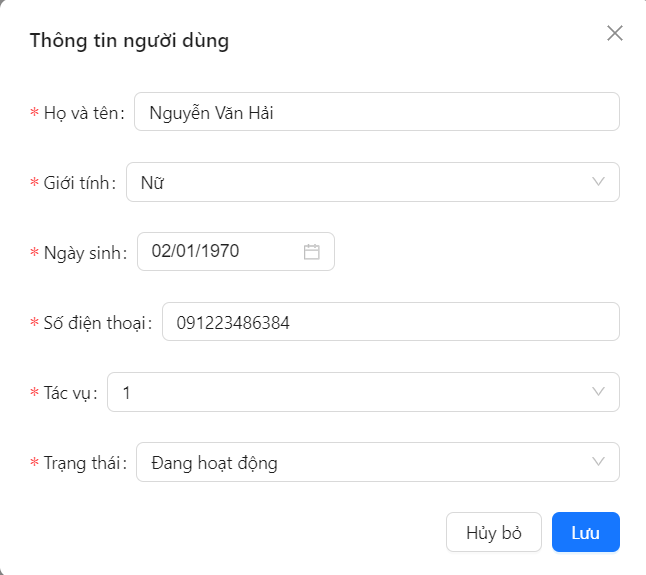
\includegraphics[scale=0.7]{Images/server/webUI/updateUser.png}
  \caption[Giao diện màn cập nhật thông tin người dùng]{\bfseries \fontsize{12pt}{0pt}\selectfont Giao diện màn cập nhật thông tin người dùng}
  \label{editUser} %đặt tên cho ảnh
\end{figure}

Hình \ref{editUser} mô tả giao diện cho màn cập nhật thông tin người dùng. Màn này sẽ có các trường thông tin bao gồm 
tên, giới tính, ngày sinh, số điện thoại, tác vụ, trạng thái. Trên các trường sẽ hiện thông tin người dùng mà admin đã chọn. 
Admin sẽ chỉnh sửa thông tin, sau đó nhấn nút Lưu để lưu dữ liệu.

\begin{figure}[H]
  \centering
  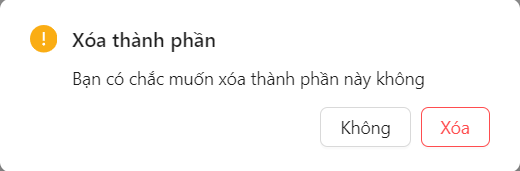
\includegraphics[scale=0.7]{Images/server/webUI/delete.png}
  \caption[Giao diện màn xóa thông tin trong trang quản lý]{\bfseries \fontsize{12pt}{0pt}\selectfont Giao diện màn xóa thông tin trong trang quản lý}
  \label{delete} %đặt tên cho ảnh
\end{figure}

Hình \ref{delete} mô tả giao diện cho màn xóa thông tin trong trang quản lý. Màn này sẽ hiện lên thông tin xác nhận người dùng có muốn 
xóa trường thông tin ấy không. Nếu người dùng muốn xóa sẽ nhấn nút Xóa, còn nếu không sẽ nhấn nút Hủy bỏ.

\begin{figure}[H]
  \centering
  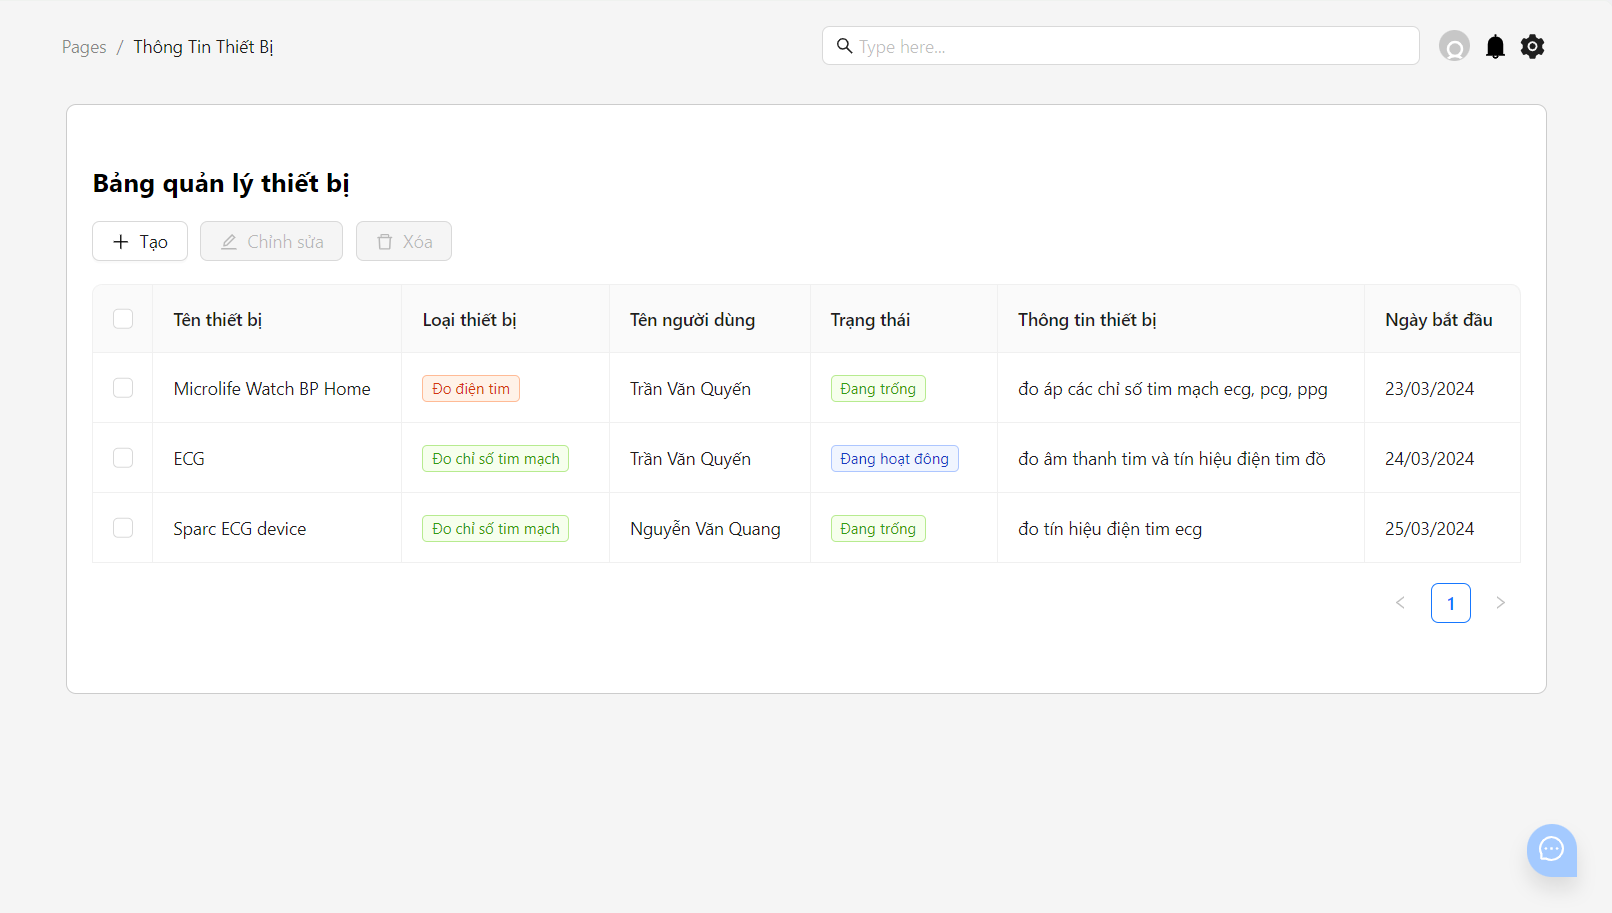
\includegraphics[scale=0.5]{Images/server/webUI/deviceTable.png}
  \caption[Giao diện trang quản lý thiết bị]{\bfseries \fontsize{12pt}{0pt}\selectfont Giao diện trang quản lý thiết bị}
  \label{deviceTable} %đặt tên cho ảnh
\end{figure}

Hình \ref{deviceTable} mô tả giao diện cho trang quản lý người dùng, trang này sẽ hiển thị danh sách
thông tin của các thiết bị đang có trên hệ thống, bên cạnh đó khi tích vào mỗi thiết bị tương ứng sẽ 
có các lựa chọn để xem chi tiết thông tin thiết bị, cập nhật thông
tin hay xóa thông tin. Và ở trang này sẽ có thêm các nút bấm để tạo mới thông tin thiết bị.

\begin{figure}[H]
  \centering
  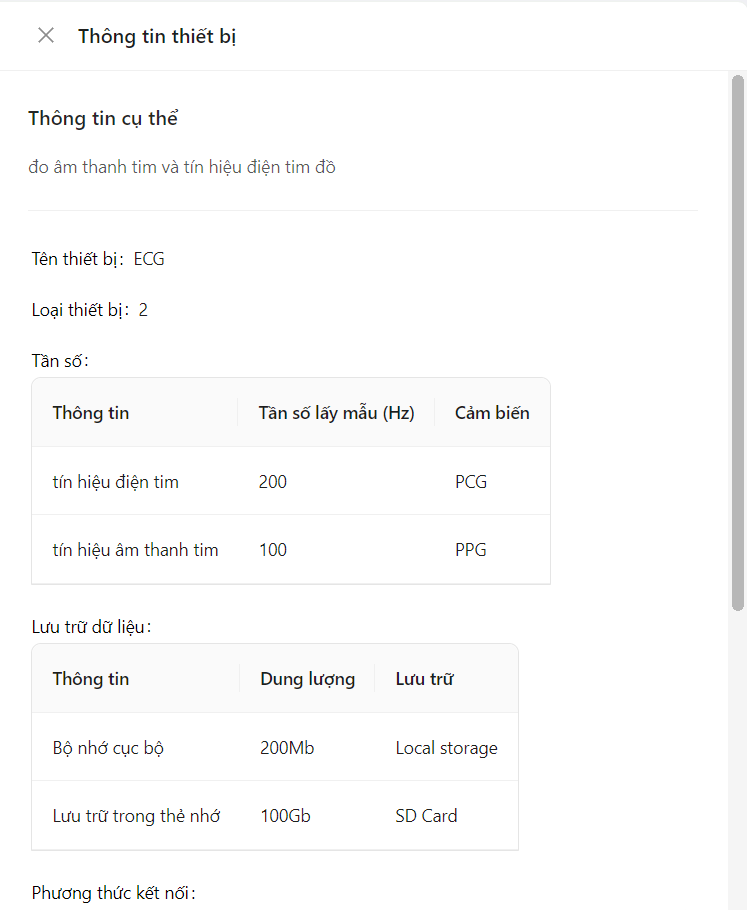
\includegraphics[scale=0.7]{Images/server/webUI/deviceInfo_1.png}
  \caption[Giao diện màn thông tin chi tiết thiết bị]{\bfseries \fontsize{12pt}{0pt}\selectfont Giao diện màn thông tin chi tiết thiết bị}
  \label{deviceInfo} %đặt tên cho ảnh
\end{figure}

Hình \ref{deviceInfo} mô tả giao diện cho màn thông tin chi tiết thiết bị, màn này sẽ hiển thị thông tin
chi tiết của thiết bị khi quản trị viên chọn vào một thiết bị trong danh sách.

\begin{figure}[H]
  \centering
  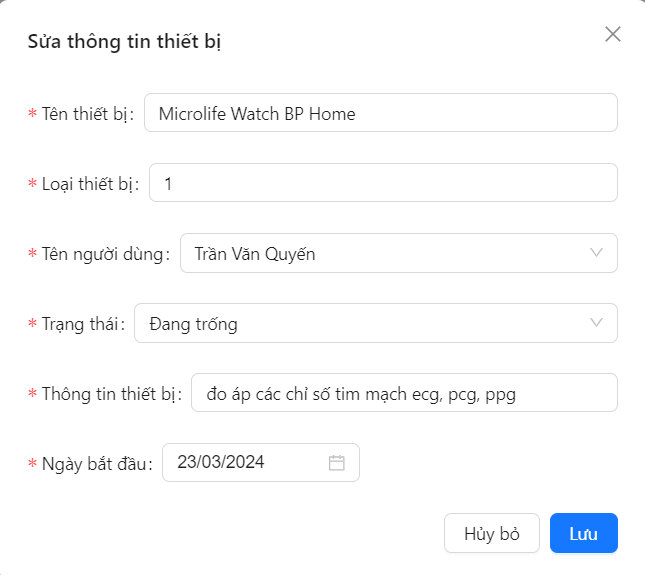
\includegraphics[scale=0.7]{Images/server/webUI/editDevice.png}
  \caption[Giao diện màn cập nhật thông tin thiết bị]{\bfseries \fontsize{12pt}{0pt}\selectfont Giao diện màn cập nhật thông tin thiết bị}
  \label{editDevice} %đặt tên cho ảnh
\end{figure}

Hình \ref{editDevice} mô tả giao diện cho màn cập nhật thông tin thiết bị. Màn này sẽ có các trường thông tin bao gồm 
tên thiết bị, loại thiết bị, tên người dùng, trạng thái, thông tin, ngày bắt đầu. Trên các trường sẽ hiện thông tin thiết bị mà quản trị viên đã chọn. 
Admin sẽ chỉnh sửa thông tin, sau đó nhấn nút Lưu để lưu dữ liệu.

\begin{figure}[H]
  \centering
  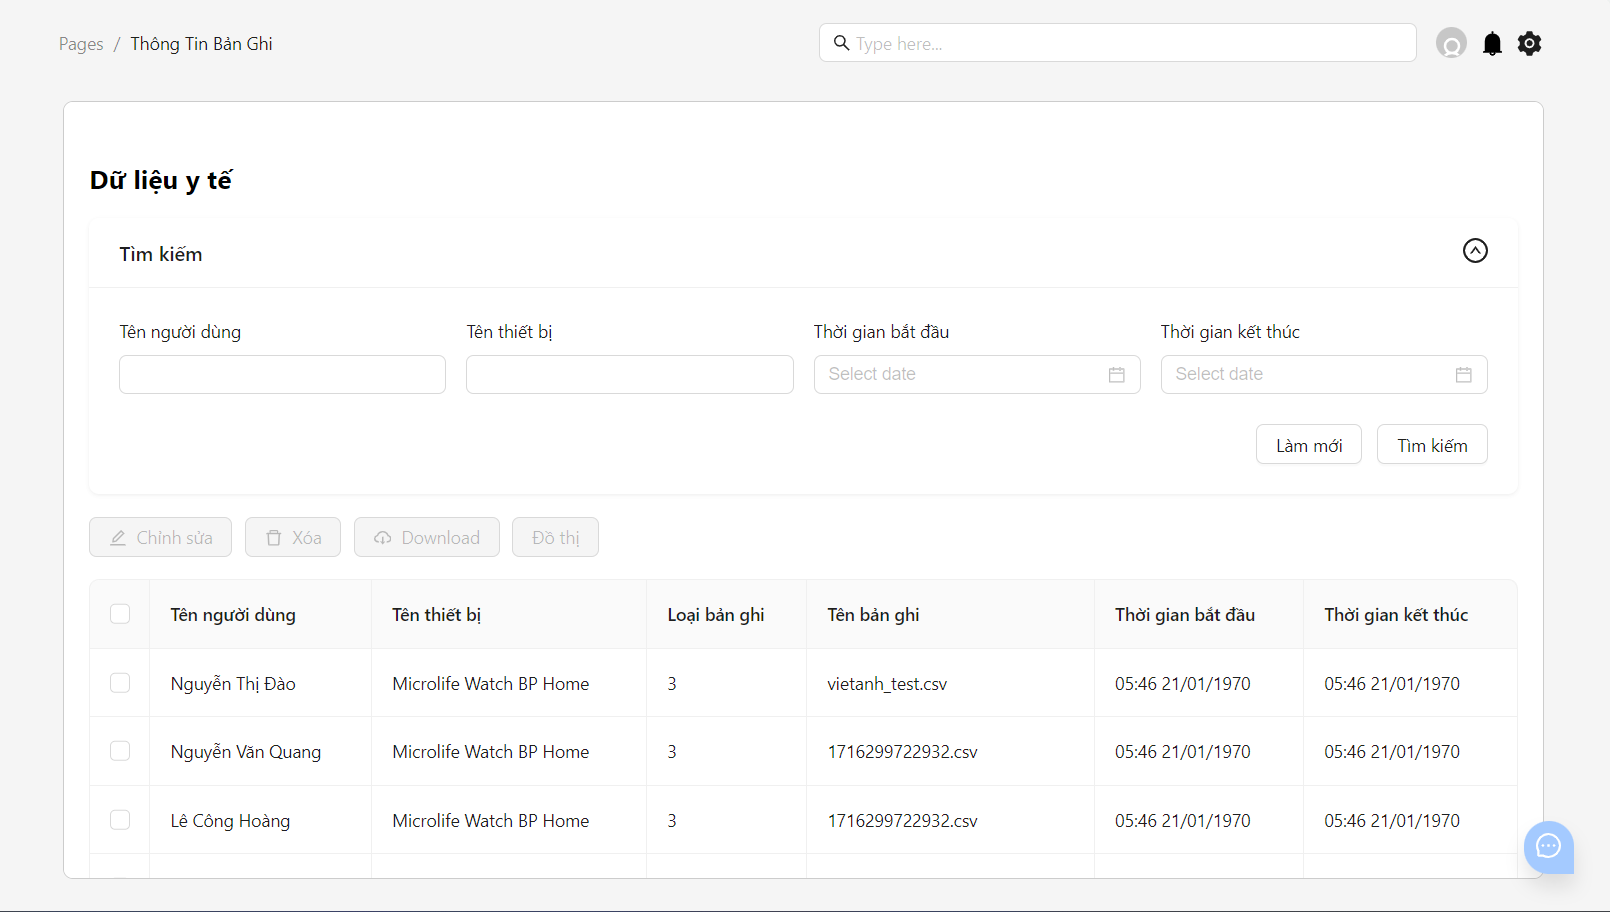
\includegraphics[scale=0.5]{Images/server/webUI/recordTable.png}
  \caption[Giao diện trang quản lý phiên đo]{\bfseries \fontsize{12pt}{0pt}\selectfont Giao diện trang quản lý phiên đo}
  \label{recordTable} %đặt tên cho ảnh
\end{figure}

Hình \ref{recordTable} mô tả giao diện cho trang quản lý phiên đo, trang này sẽ hiển thị danh sách
thông tin của các phiên đo trên hệ thống, bên cạnh đó khi tích vào mỗi phiên đo tương ứng sẽ 
có các lựa chọn để cập nhật thông tin, xóa thông tin, tải bản ghi cũng như xem đồ thị phiên đo. 

\begin{figure}[H]
  \centering
  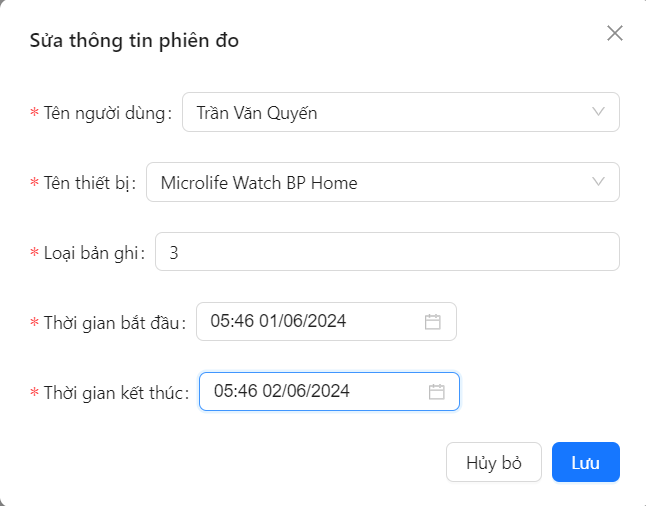
\includegraphics[scale=0.7]{Images/server/webUI/editRecord.png}
  \caption[Giao diện màn cập nhật thông tin phiên đo]{\bfseries \fontsize{12pt}{0pt}\selectfont Giao diện màn cập nhật thông tin phiên đo}
  \label{editRecord} %đặt tên cho ảnh
\end{figure}

Hình \ref{editRecord} mô tả giao diện cho màn cập nhật thông tin thiết bị. Màn này sẽ có các trường thông tin bao gồm 
tên người dùng, tên thiết bị, loại bản ghi, thời gian bắt đầu, thời gian kết thúc. Trên các trường sẽ hiện thông tin phiên đo mà quản trị viên đã chọn. 
Admin sẽ chỉnh sửa thông tin, sau đó nhấn nút Lưu để lưu dữ liệu.

\begin{figure}[H]
  \centering
  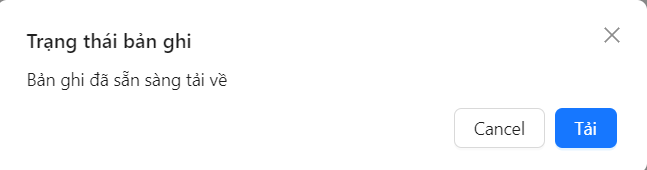
\includegraphics[scale=0.7]{Images/server/webUI/downloadRecord.png}
  \caption[Giao diện màn tải bản ghi dữ liệu phiên đo]{\bfseries \fontsize{12pt}{0pt}\selectfont Giao diện màn tải bản ghi dữ liệu phiên đo}
  \label{downloadRecord} %đặt tên cho ảnh
\end{figure}

Hình \ref{downloadRecord} mô tả giao diện cho màn tải bản ghi dữ liệu phiên đo. Màn này sẽ hiện lên thông tin xác nhận người dùng có muốn 
tải bản ghi dữ liệu phiên đo không cũng như trạng thái tải. Nếu người dùng muốn tải bản ghi sẽ nhấn nút Tải, còn nếu không sẽ nhấn nút Hủy bỏ.

\begin{figure}[H]
  \centering
  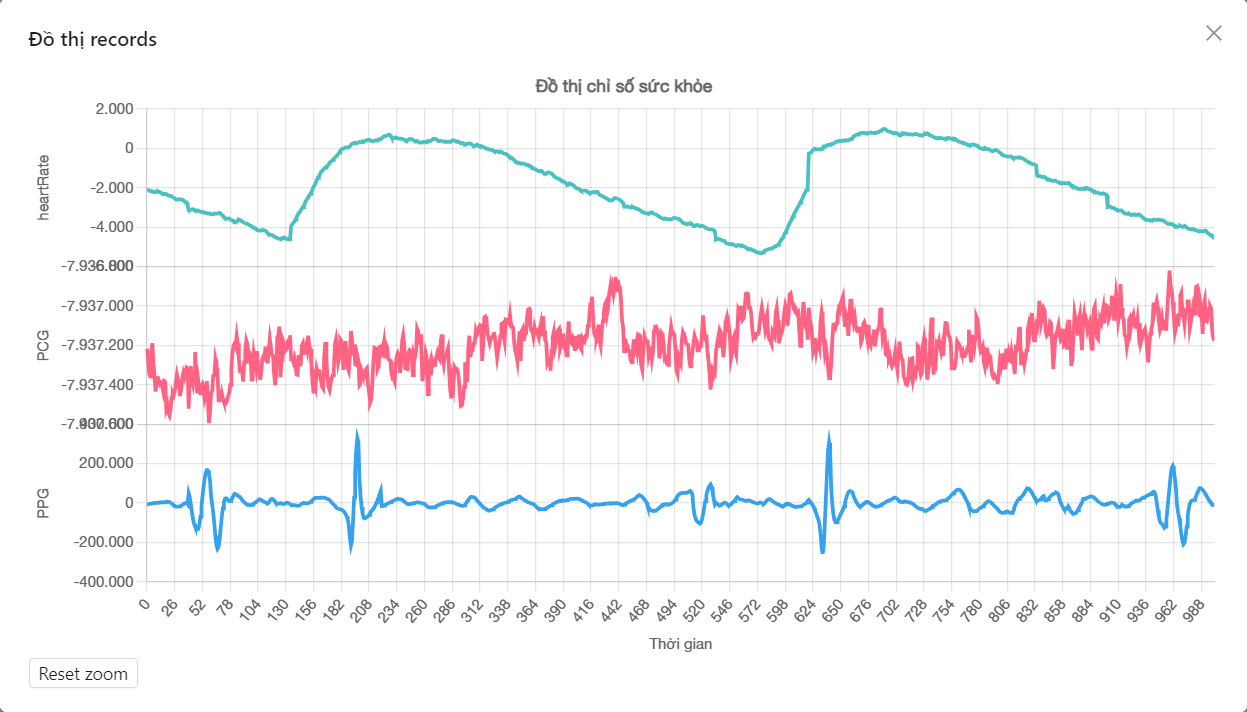
\includegraphics[scale=0.6]{Images/server/webUI/chart.png}
  \caption[Giao diện màn biểu đồ dữ liệu phiên đo]{\bfseries \fontsize{12pt}{0pt}\selectfont Giao diện màn biểu đồ dữ liệu phiên đo}
  \label{recordChart} %đặt tên cho ảnh
\end{figure}

Hình \ref{recordChart} mô tả giao diện cho màn biểu đồ dữ liệu phiên đo. Màn này sẽ hiện lên thông tin dữ liệu phiên đo theo biểu đồ đường, người dùng 
có thể phóng to thu nhỏ. Nếu có nhiều hơn một dữ liệu đo, thể hiện qua màu sắc các đường và trục tung sẽ hiển thị tên kênh đo dữ liệu giúp người dùng dễ dàng theo dõi.

\begin{figure}[H]
  \centering
  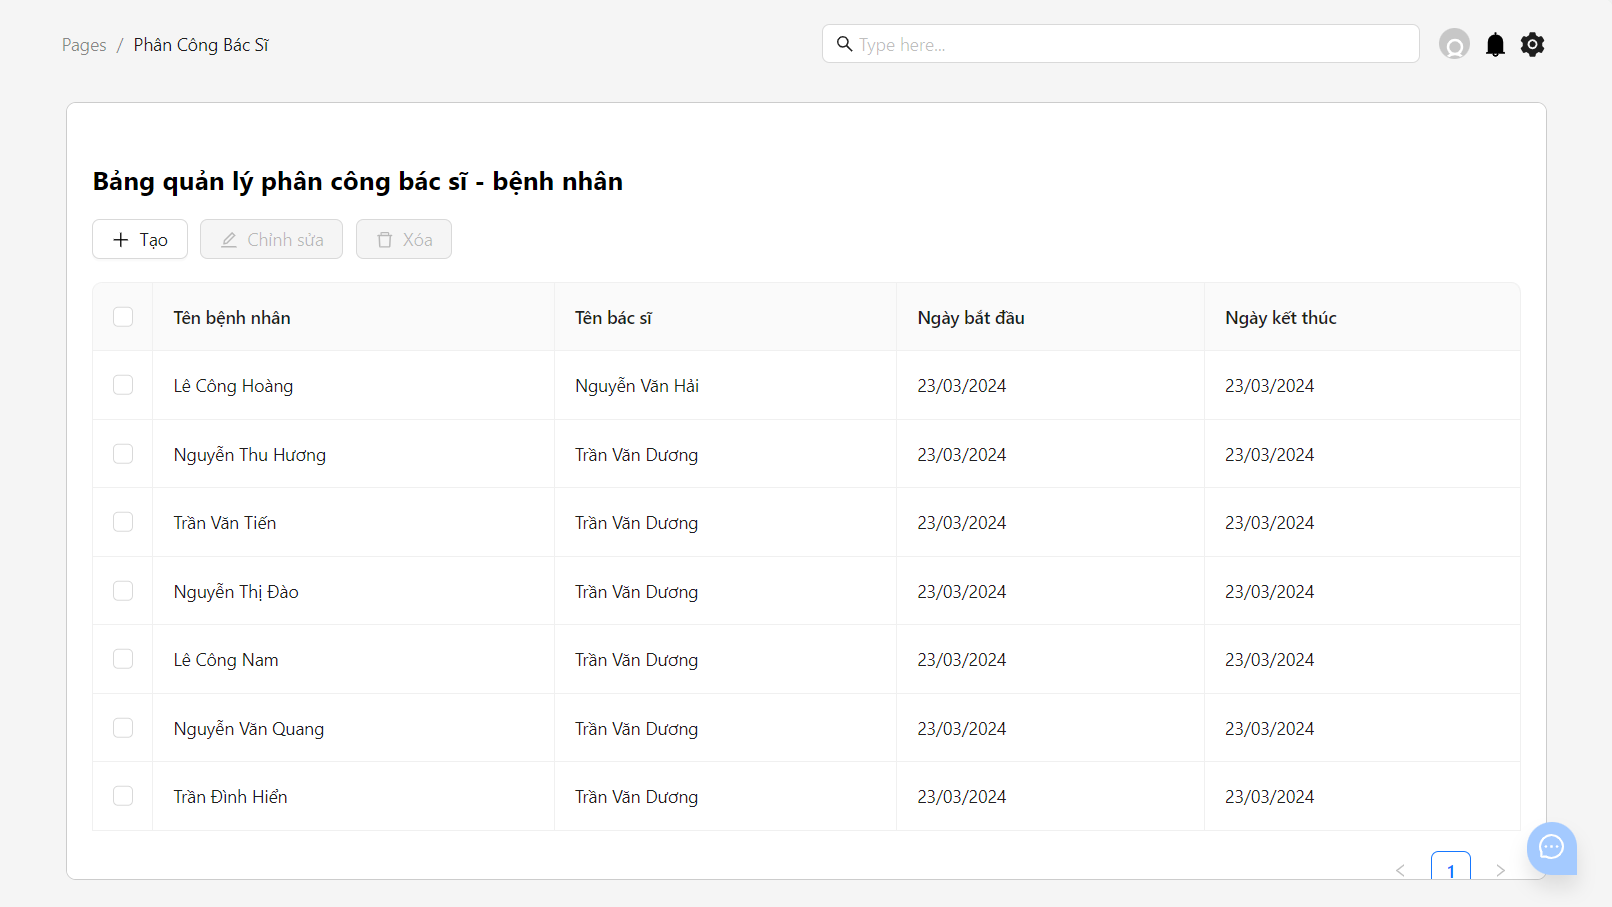
\includegraphics[scale=0.5]{Images/server/webUI/pdaTable.png}
  \caption[Giao diện trang quản lý phân công bác sĩ - bệnh nhân]{\bfseries \fontsize{12pt}{0pt}\selectfont Giao diện trang quản lý phân công bác sĩ - bệnh nhân}
  \label{pdaTable} %đặt tên cho ảnh
\end{figure}

Hình \ref{pdaTable} mô tả giao diện cho trang quản lý phân công bác sĩ - bệnh nhân, trang này sẽ hiển thị danh sách
thông tin của các phân công trên hệ thống, bên cạnh đó khi tích vào mỗi phân công tương ứng sẽ 
có các lựa chọn để cập nhật thông tin, xóa thông tin, bên cạnh đó sẽ có nút tạo phân công mới. 

\begin{figure}[H]
  \centering
  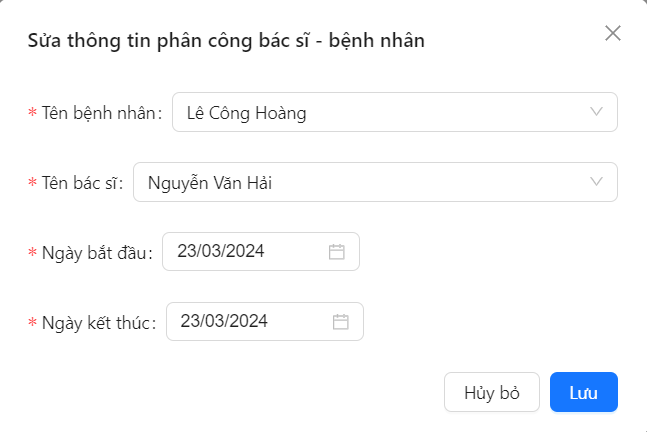
\includegraphics[scale=0.7]{Images/server/webUI/editPDA.png}
  \caption[Giao diện màn cập nhật thông tin phân công bác sĩ - bệnh nhân]{\bfseries \fontsize{12pt}{0pt}\selectfont Giao diện màn cập nhật thông tin phân công bác sĩ - bệnh nhân}
  \label{editPDA} %đặt tên cho ảnh
\end{figure}

Hình \ref{editPDA} mô tả giao diện cho màn cập nhật thông tin phân công bác sĩ - bệnh nhân. Màn này sẽ có các trường thông tin bao gồm 
tên bác sĩ, tên bệnh nhân, ngày bắt đầu, ngày kết thúc. Trên các trường sẽ hiện thông tin phân công mà quản trị viên đã chọn. 
Admin sẽ chỉnh sửa thông tin, sau đó nhấn nút Lưu để lưu dữ liệu.

\begin{figure}[H]
  \centering
  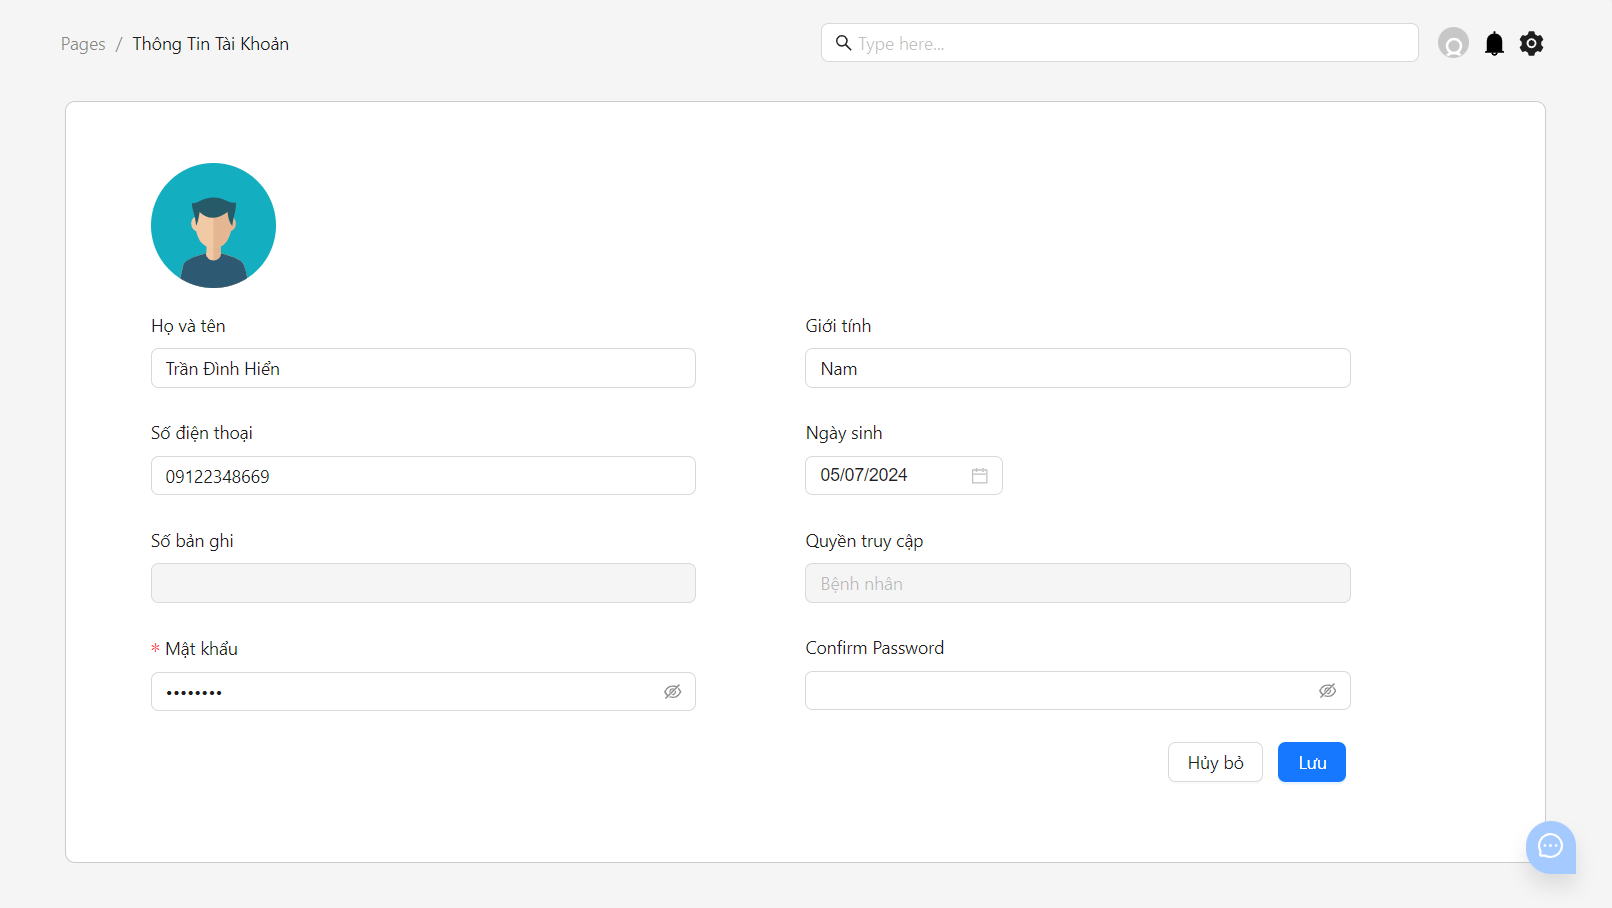
\includegraphics[scale=0.5]{Images/server/webUI/accountInfo.png}
  \caption[Giao diện trang thông tin tài khoản]{\bfseries \fontsize{12pt}{0pt}\selectfont Giao diện màn cập nhật thông tin phân công bác sĩ - bệnh nhân}
  \label{accountInfo} %đặt tên cho ảnh
\end{figure}

Hình \ref{accountInfo} mô tả giao diện cho trang thông tin tài khoản. Trang này sẽ có các trường thông tin bao gồm 
họ và tên, giới tính, số điện thoại, ngày sinh, số bản ghi, quyền truy cập, mật khẩu và xác nhận mật khẩu. Trên các trường sẽ hiện thông tin của tài khoản. 
Người dùng sẽ chỉnh sửa thông tin, sau đó nhấn nút Lưu để lưu dữ liệu.

\begin{figure}[H]
  \centering
  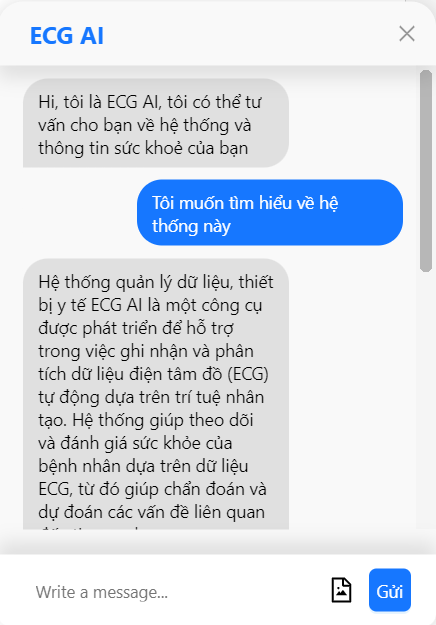
\includegraphics[scale=0.5]{Images/server/webUI/chat_ai.png}
  \caption[Giao diện màn hỏi, nhận tư vấn từ AI]{\bfseries \fontsize{12pt}{0pt}\selectfont Giao diện màn hỏi, nhận tư vấn từ AI}
  \label{chatAI} %đặt tên cho ảnh
\end{figure}

Hình \ref{chatAI} mô tả giao diện cho màn hỏi, nhận tư vấn từ AI. Khi người dùng nhấn vào nút ở góc phải màn hình sẽ hiện lên màn chat với AI. 
Người dùng có thể bắt đầu nhắn tin ở thanh nhắn tin, các tin nhắn sẽ hiển thị theo thứ tự trên xuống. Khi người dùng nhắn một tin, tin nhắn sẽ hiện ở dưới cùng và 
có màu xanh, còn tin nhắn phản hồi từ AI sẽ có nền màu xám. 

\begin{figure}[H]
  \centering
  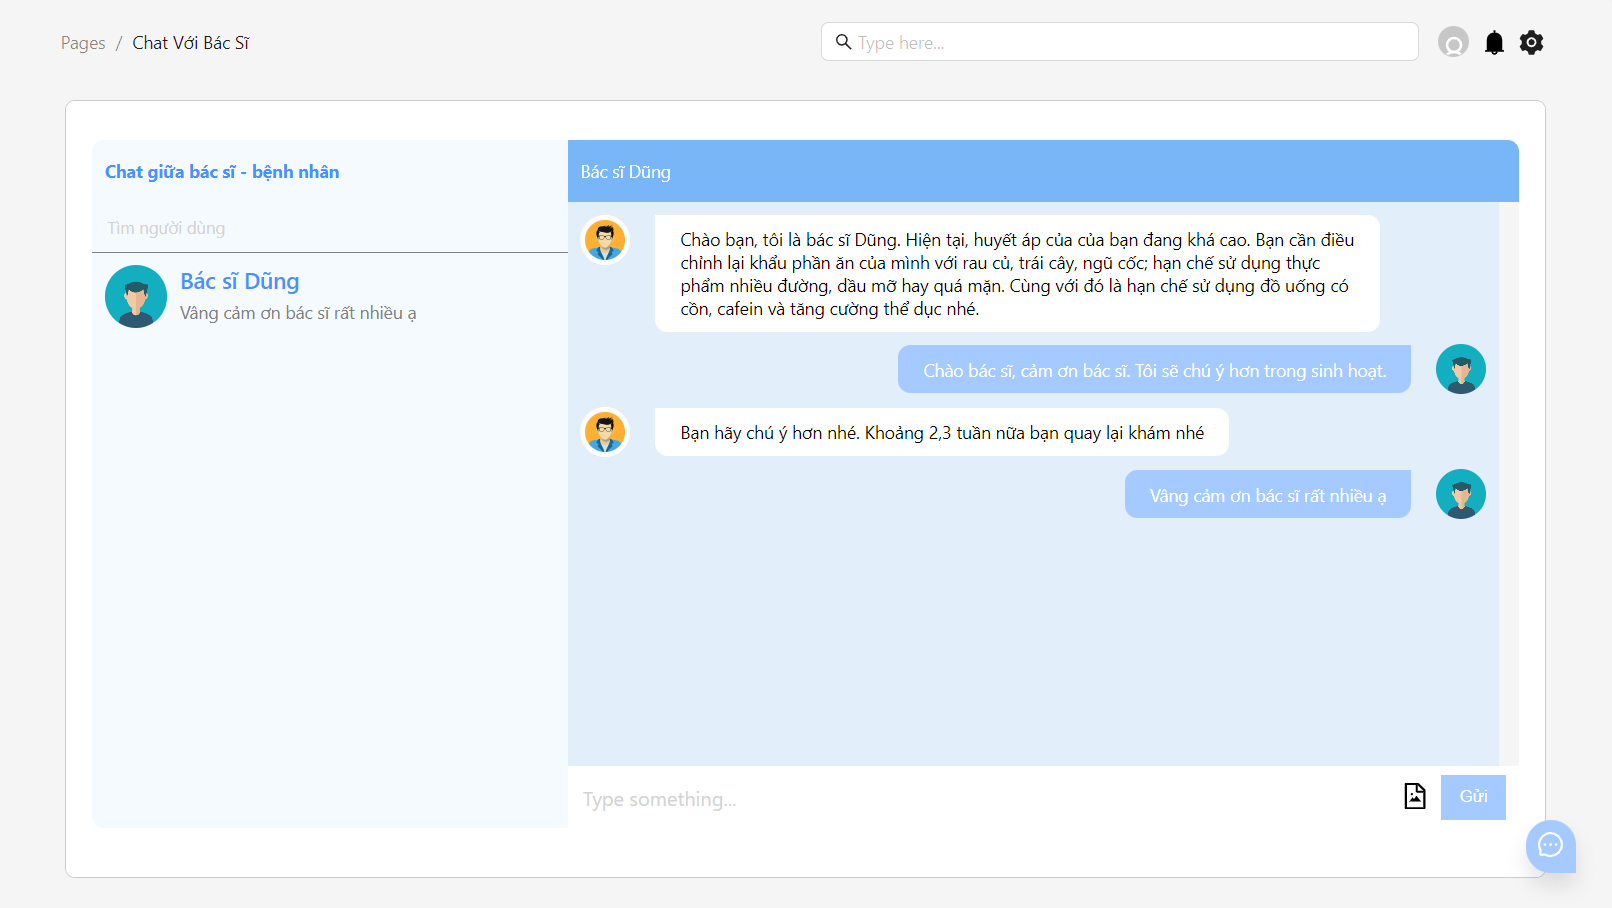
\includegraphics[scale=0.5]{Images/server/webUI/chat.png}
  \caption[Giao diện trang chi tiết hội thoại bệnh nhân, bác sĩ]{\bfseries \fontsize{12pt}{0pt}\selectfont Giao diện trang hỏi, nhận tư vấn từ AI}
  \label{chat} %đặt tên cho ảnh
\end{figure}

Hình \ref{chat} mô tả giao diện cho trang chi tiết hội thoại bệnh nhân, bác sĩ. Ở trong trang này, phía bên trái là danh sách các bệnh nhân, bác sĩ 
bao gồm tên và tin nhắn cuối mà người dùng đã trò chuyện, bên phải là nội dung chi tiết cuộc hội thoại. Người dùng có thể bắt đầu nhắn tin ở thanh nhắn tin 
có thể đính kèm tệp hình ảnh, các tin nhắn sẽ hiển thị theo thứ tự trên xuống. Khi người dùng nhắn một tin, tin nhắn sẽ hiện ở dưới cùng và 
có màu xanh, còn tin nhắn phản hồi từ AI sẽ có nền màu xám. 

\subsection{Thiết kế các chức năng cho website và server}

\subsubsection{Thiết kế API}


\begin{enumerate}[a)]
  \item API liên quan đến việc xác thực người dùng


\begin{table}[H]
  \centering
  \caption{\bfseries \fontsize{12pt}{0pt}\selectfont Bảng API liên quan đến việc xác thực người dùng}
  \begin{tabularx}{0.9\textwidth}{
  | >{\raggedright\arraybackslash}X
  | >{\raggedright\arraybackslash}m{2cm}
  | >{\raggedright\arraybackslash}X|
  }
  \hline
  \bfseries Đường dẫn    &\bfseries Phương thức    &\bfseries Mô tả\\ \hline
  api/auth/register   &   POST  & Đăng ký tài khoản \\ \hline
  api/auth/login   &    POST    & Đăng nhập vào hệ thống \\ \hline
  api/auth/logout   &    POST    & Đăng xuất khỏi hệ thống \\ \hline
  api/auth/reset-password  &     POST   &  Gửi reset link đến email của người dùng để reset mật khẩu \\  \hline
  api/auth/reset-password/reset &   POST     & Giúp reset lại mật khẩu mới với verify token được nhận từ api: api/reset-password  \\ \hline

  \end{tabularx}
  \label{table_api_auth}
\end{table}

  \item API liên quan đến việc đăng ký tài khoản


\begin{table}[H]
  \centering
  \caption{\bfseries \fontsize{12pt}{0pt}\selectfont Bảng API liên quan đến việc đăng ký tài khoản}
  \begin{tabularx}{0.9\textwidth}{
  | >{\raggedright\arraybackslash}X
  | >{\raggedright\arraybackslash}m{2cm}
  | >{\raggedright\arraybackslash}X|
  }
  \hline
  \bfseries Đường dẫn    &\bfseries Phương thức    &\bfseries Mô tả\\ \hline
  api/register/list   &   GET  & Lấy danh sách các tài khoản đăng ký đang chờ phê duyệt \\ \hline
  api/register/accepted   &    POST    & Phê duyệt tài khoản đăng ký \\ \hline
  api/register/rejected  &     POST   &  Từ chối phê duyệt tài khoản đăng ký \\  \hline

  \end{tabularx}
  \label{table_api_register}
\end{table}

  \item API liên quan đến thông tin người dùng
  

  \begin{table}[H]
    \centering
    \caption{\bfseries \fontsize{12pt}{0pt}\selectfont Bảng API liên quan đến thông tin người dùng}
    \begin{tabularx}{0.9\textwidth}{
    | >{\raggedright\arraybackslash}X
    | >{\raggedright\arraybackslash}m{2cm}
    | >{\raggedright\arraybackslash}X|
    }
    \hline
    \bfseries Đường dẫn    &\bfseries Phương thức    &\bfseries Mô tả\\ \hline
   api/user   &   GET  &  Lấy danh sách thông tin của tất cả người dùng \\  \hline
   api/user/id/\{:userId\}  &   GET     & Lấy thông tin cụ thể của người dùng theo Id \\ \hline
   api/user/role/\{:role\}  &   GET     & Lấy danh sách người dùng theo chức vụ \\ \hline
   api/user/update   &    POST    &  Cập nhật thông tin người dùng \\  \hline
   api/user/delete/\{:userId\}  &   DELETE     & Xóa thông tin người dùng theo Id \\ \hline

    \end{tabularx}
    \label{table_api_user}
\end{table}

\item API liên quan đến chat


\begin{table}[H]
  \centering
  \caption{\bfseries \fontsize{12pt}{0pt}\selectfont Bảng API liên quan đến tin tức}
  \begin{tabularx}{0.9\textwidth}{
  | >{\raggedright\arraybackslash}X
  | >{\raggedright\arraybackslash}m{2cm}
  | >{\raggedright\arraybackslash}X|
  }
  \hline
  \bfseries Đường dẫn    &\bfseries Phương thức    &\bfseries Mô tả\\ \hline

  \end{tabularx}
  \label{table_api_chats}
\end{table}
\item API liên quan đến quản lý thiết bị


\begin{table}[H]
  \centering
  \caption{\bfseries \fontsize{12pt}{0pt}\selectfont Bảng API liên quan đến quản lý thiết bị}
  \begin{tabularx}{0.9\textwidth}{
  | >{\raggedright\arraybackslash}X
  | >{\raggedright\arraybackslash}m{2cm}
  | >{\raggedright\arraybackslash}X|
  }
  \hline
  \bfseries Đường dẫn    &\bfseries Phương thức    &\bfseries Mô tả\\ \hline
 api/device   &   GET  & Lấy danh sách thông tin tất cả thiết bị \\ \hline
 api/devide/\{:deviceId\}   &    GET    & Lấy thông tin của một thiết bị \\ \hline
 api/device/add &   POST     & Thêm thông tin thiết bị mới \\ \hline
 api/device/update  &     POST   & Cập nhật thông tin một thiết bị \\ \hline
 api/device/delete/\{:deviceId\}  &     DELETE   & Xóa thông tin một thiết bị theo Id \\ \hline

  \end{tabularx}
  \label{table_api_device}
\end{table}

\item API liên quan đến bản ghi ECG


\begin{table}[H]
  \centering
  \caption{\bfseries \fontsize{12pt}{0pt}\selectfont Bảng API liên quan đến bản ghi ECG}
  \begin{tabularx}{0.9\textwidth}{
  | >{\raggedright\arraybackslash}X
  | >{\raggedright\arraybackslash}m{2cm}
  | >{\raggedright\arraybackslash}X|
  }
  \hline
  \bfseries Đường dẫn    &\bfseries Phương thức    &\bfseries Mô tả\\ \hline
 api/record   &   GET  & Lấy danh sách thông tin các phiên đo ECG \\ \hline
 api/record/user/\{:userId\}   &    GET    & Lấy danh sách thông tin các phiên đo ECG của bệnh nhân \\ \hline
 api/record/doctor/\{:doctorId\} &   GET     & Lấy danh sách thông tin các phiên đo ECG của các bệnh nhân được quản lý bởi bác sỹ \\ \hline
 api/record/id/\{:recordId\}  &     GET   & Lấy thông tin một phiên đo của bệnh nhân \\ \hline
 api/record/getData/\{:recordId\}  &     GET   & Lấy dữ liệu một phiên đo của bệnh nhân \\ \hline
 api/ record/download/\{:recordId\}  &     GET   & Tải dữ liệu một phiên đo của bệnh nhân \\ \hline
 api/record/update  &     POST   & Cập nhật thông tin một phiên đo của bệnh nhân \\ \hline
 api/record/delete/\{:recordId\}  &     DELETE   & Xóa thông tin một phiên đo của bệnh nhân \\ \hline

  \end{tabularx}
  \label{table_api_ecg}
\end{table}


\item API liên quan liên quan đến việc phân công bệnh nhân cho bác sỹ

\begin{table}[H]
  \centering
  \caption{\bfseries \fontsize{12pt}{0pt}\selectfont Bảng API liên quan liên quan đến việc phân công bệnh nhân cho bác sỹ}
  \begin{tabularx}{0.9\textwidth}{
  | >{\raggedright\arraybackslash}X
  | >{\raggedright\arraybackslash}m{2cm}
  | >{\raggedright\arraybackslash}X|
  }
  \hline
  \bfseries Đường dẫn    &\bfseries Phương thức    &\bfseries Mô tả\\ \hline
  api/pda   &   GET  & Lấy danh sách tất cả thông tin phân công bác sĩ - bệnh nhân \\ \hline
  api/pda/create  &    POST    & Tạo một phân công bác sĩ - bệnh nhân mới \\ \hline
  api/pda/update  &    POST    & Cập nhật thông tin một phân công bác sĩ - bệnh nhân mới \\ \hline
  api/pda/delete/\{:deviceId\}  &    DELETE    & Xóa một phân công bác sĩ - bệnh nhân mới \\ \hline
  api/pda/patient/\{:doctorId\} &  GET  & Lấy danh sách tất cả bệnh nhân theo ID bác sĩ \\ \hline
  api/pda/doctor/\{:patientId\} &  GET  & Lấy danh sách tất cả bác sĩ theo ID bệnh nhân \\ \hline


  \end{tabularx}
  \label{table_api_pda}
\end{table}



\end{enumerate}




\subsubsection{Sơ đồ tuần tự}

% ------------------------Auth----------------------


\paragraph{API liên quan đến việc xác thực người dùng}
\mbox{}

\begin{figure}[H]
  \centering
  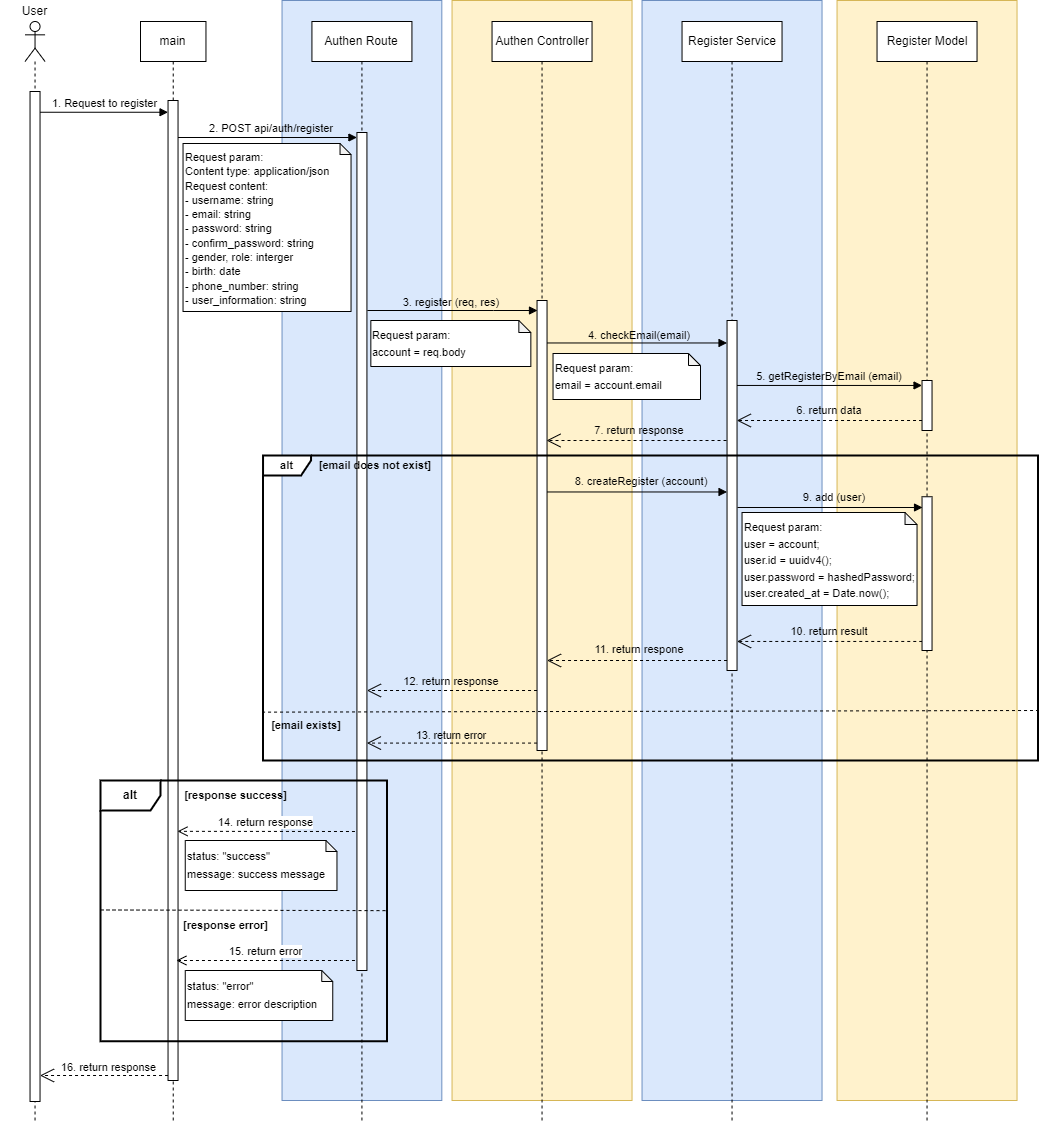
\includegraphics[width=16cm,height=15cm]{Images/sequence_api/register.png}
  \caption[Sơ đồ tuần tự cho API đăng ký tài khoản vào hệ thống]{\bfseries \fontsize{12pt}{0pt}
  \selectfont Sơ đồ tuần tự cho API đăng ký tài khoản vào hệ thống }
  \label{api_register} %đặt tên cho ảnh
\end{figure}
Hình \ref{api_register}  mô tả quá trình xác thực người dùng đăng ký tài khoản. Người dùng gửi yêu cầu đăng ký, thông qua các tầng của hệ thống, yêu cầu này được xử lý bởi AutheController. AuthenController kiểm tra thông tin người dùng, tạo tài khoản phê duyệt 
nếu đúng thông tin đăng ký và trả về response cho người dùng.

\begin{figure}[H]
  \centering
  \includegraphics[width=16cm,height=16cm]{Images/sequence_api/login.png}
  \caption[Sơ đồ tuần tự cho API đăng nhập vào hệ thống]{\bfseries \fontsize{12pt}{0pt}
  \selectfont Sơ đồ tuần tự cho API đăng nhập vào hệ thống }
  \label{api_login} %đặt tên cho ảnh
\end{figure}
Hình \ref{api_login}  mô tả quá trình xác thực người dùng đăng ký tài khoản. Người dùng gửi yêu cầu đăng nhập, thông qua các tầng của hệ thống, yêu cầu này được xử lý bởi AutheController. AuthenController kiểm tra thông tin người dùng, tạo token truy cập và token làm mới 
nếu đúng thông tin đăng nhập và trả về response cho người dùng.

% ----------------------------------------------


% ------------------------User----------------------


\paragraph{API liên quan đến thông tin người dùng}
\mbox{}

\begin{figure}[H]
  \centering
  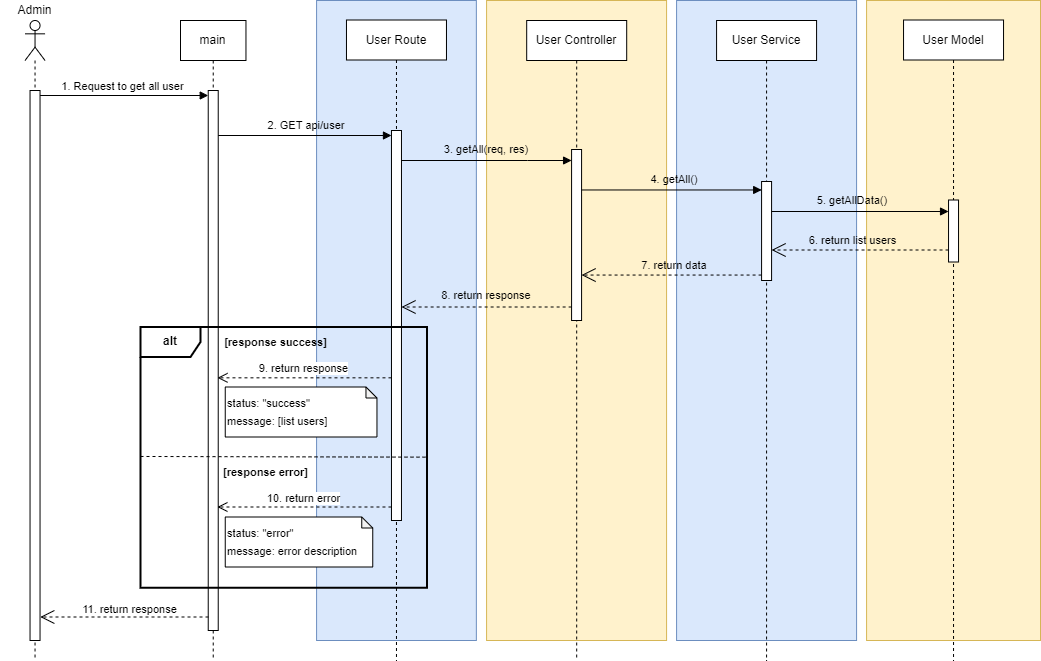
\includegraphics[width=16cm,height=9cm]{Images/sequence_api/getAllUsers.png}
  \caption[Sơ đồ tuần tự cho API lấy danh sách tất cả người dùng ]{\bfseries \fontsize{12pt}{0pt}
  \selectfont Sơ đồ tuần tự cho API lấy danh sách tất cả người dùng }
  \label{api_getAllUser} %đặt tên cho ảnh
\end{figure}
Hình \ref{api_getAllUser} mô tả quá trình lấy danh sách thông tin tất cả người dùng trong hệ thống. Người dùng gửi yêu cầu lấy danh sách người dùng, thông qua các tầng của hệ thống, yêu cầu này được xử lý bởi UserController. UserController kiểm tra thông tin và truy vấn UserModel để lấy danh sách người dùng. 
Nếu có lỗi xảy ra, hệ thống trả về response lỗi, ngược lại, response chứa danh sách thông tin người dùng được gửi lại từ UserController tới người dùng (quản trị viên).

% sửa lại ảnh 
\begin{figure}[H]
  \centering
  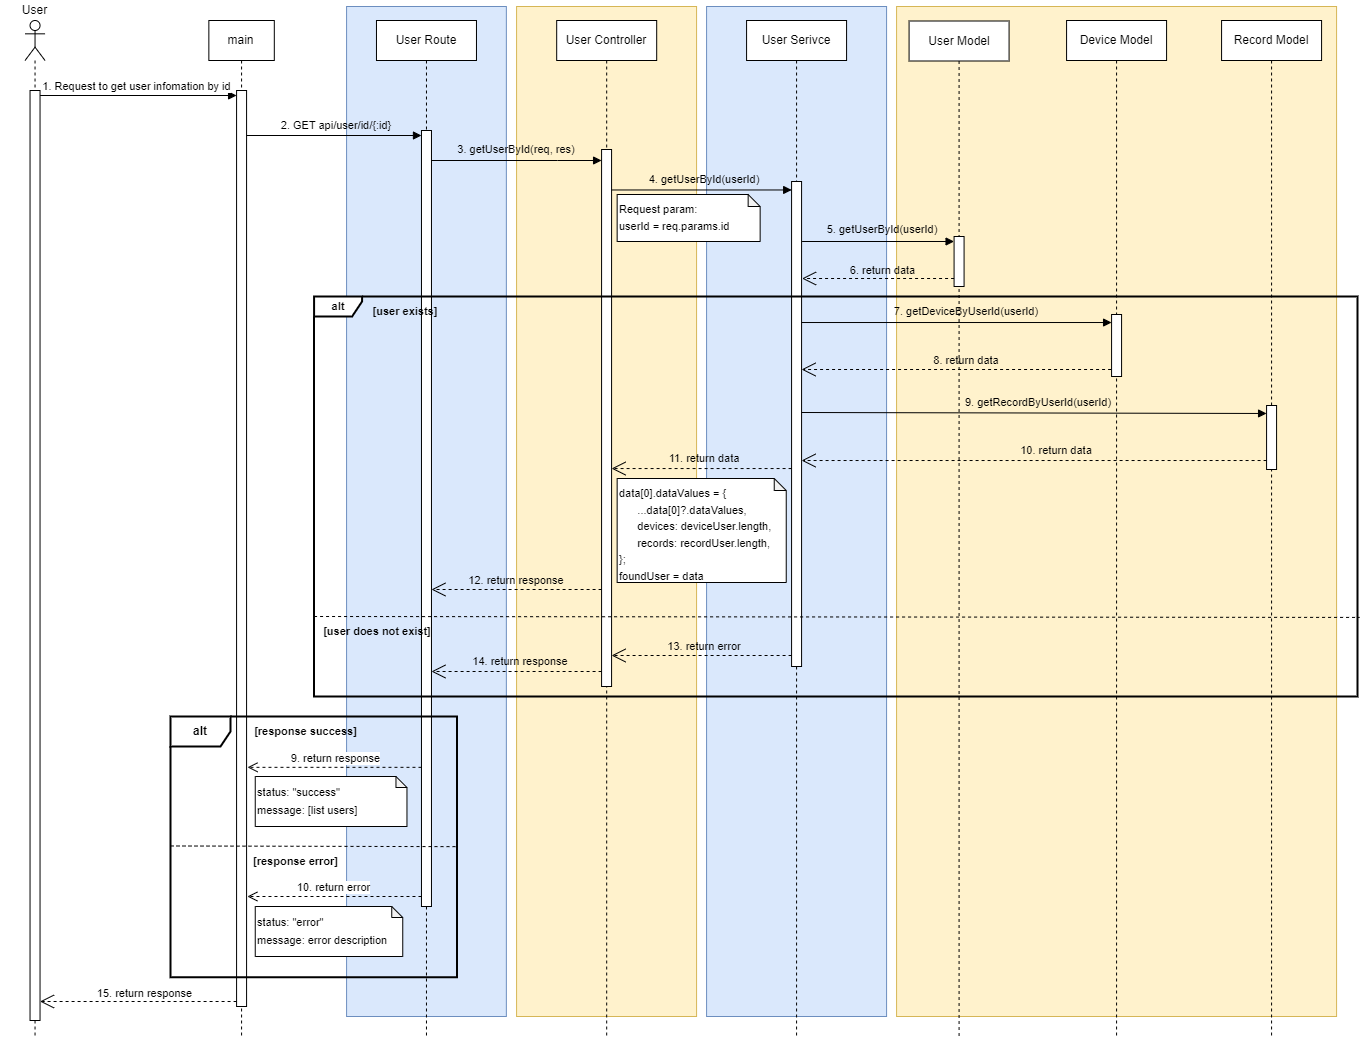
\includegraphics[width=16cm,height=11.5cm]{Images/sequence_api/getUserById.png}
  \caption[Sơ đồ tuần tự cho API lấy thông tin của người dùng dựa trên ID ]{\bfseries \fontsize{12pt}{0pt}
  \selectfont Sơ đồ tuần tự cho API lấy thông tin của người dùng dựa trên ID }
  \label{api_getUserById} %đặt tên cho ảnh
\end{figure}
Hình \ref{api_getUserById} mô tả quá trình lấy thông tin người dùng dựa trên ID trong hệ thống. Người dùng gửi yêu cầu lấy thông tin người dùng theo ID, thông qua các tầng của hệ thống, yêu cầu này được xử lý bởi UserController. UserController kiểm tra thông tin và truy vấn UserModel để lấy thông tin người dùng. 
Nếu người dùng không tồn tại, hệ thống trả về response lỗi, ngược lại, response chứa thông tin người dùng được gửi lại từ UserController tới người dùng.

\begin{figure}[H]
  \centering
  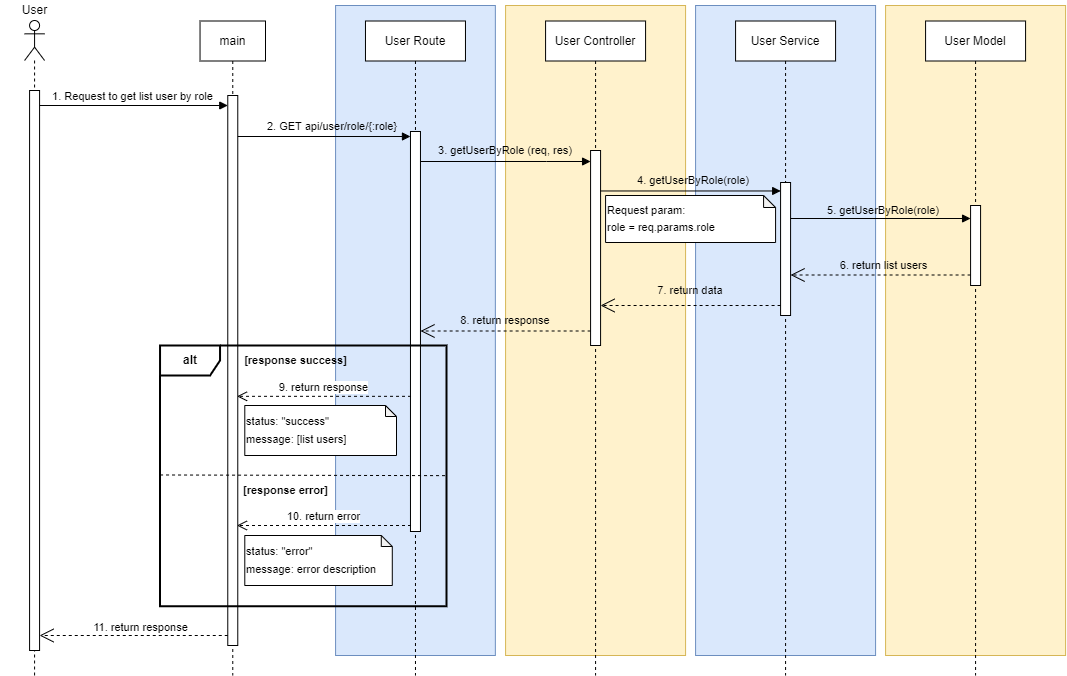
\includegraphics[width=16cm,height=10cm]{Images/sequence_api/getUserByRole.png}
  \caption[Sơ đồ tuần tự cho API lấy danh sách người dùng dựa trên chức vụ ]{\bfseries \fontsize{12pt}{0pt}
  \selectfont Sơ đồ tuần tự cho API lấy danh sách người dùng dựa trên chức vụ }
  \label{api_getUserByRole} %đặt tên cho ảnh
\end{figure}
Hình \ref{api_getUserByRole} mô tả quá trình lấy danh sách thông tin người dùng dựa trên chức vụ trong hệ thống. Người dùng gửi yêu cầu lấy danh sách người dùng theo chức vụ, thông qua các tầng của hệ thống, yêu cầu này được xử lý bởi UserController. UserController kiểm tra thông tin và truy vấn UserModel để lấy danh sách người dùng. 
Nếu có lỗi xảy ra, hệ thống trả về response lỗi, ngược lại, response chứa danh sách thông tin người dùng được gửi lại từ UserController tới người dùng.

\begin{figure}[H]
  \centering
  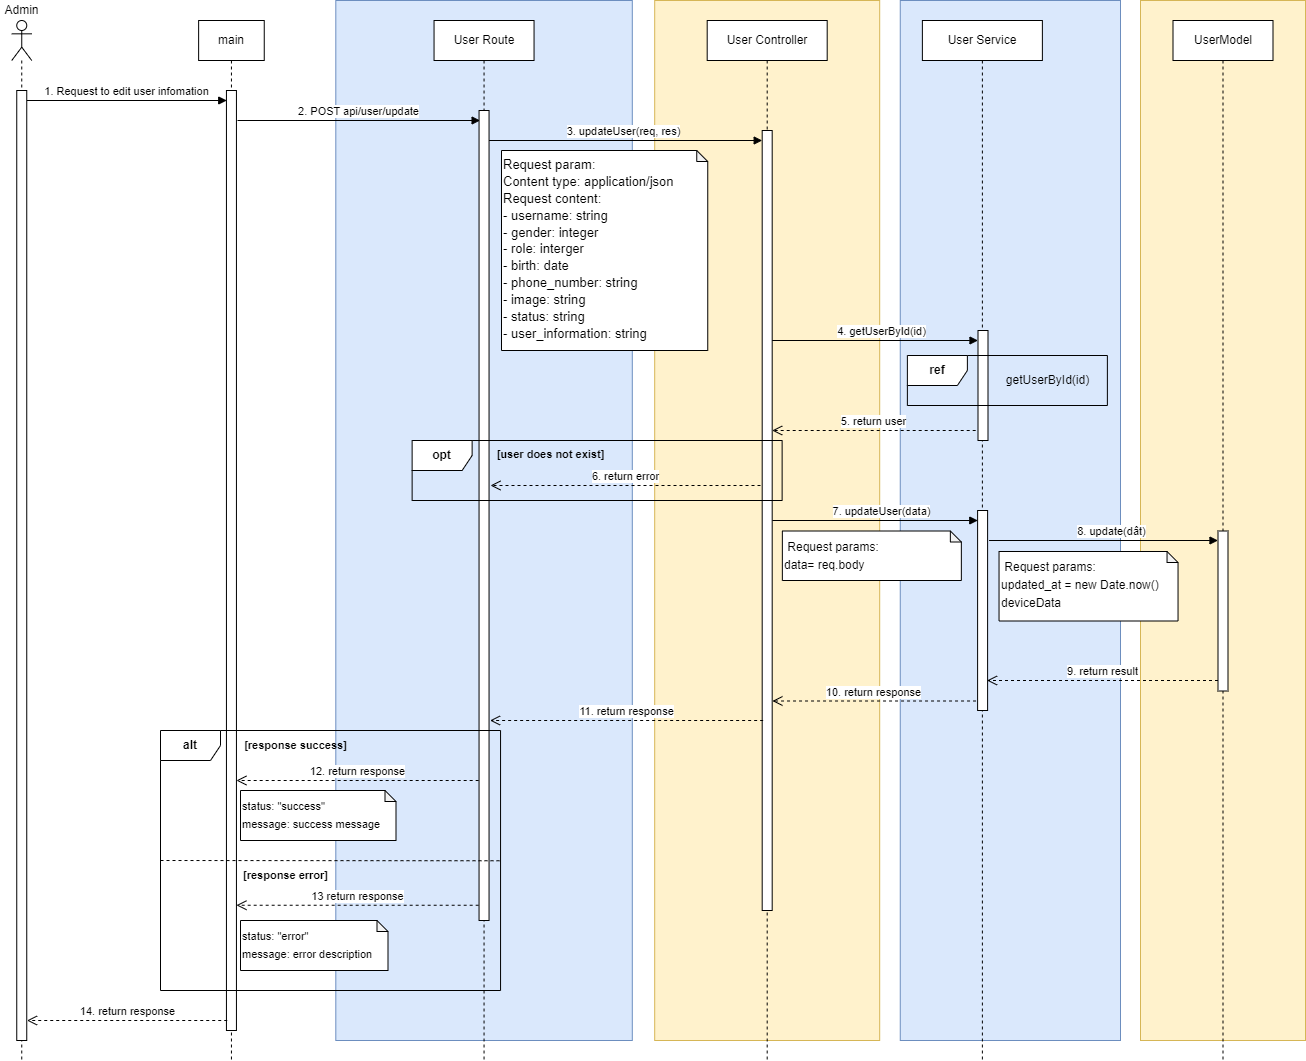
\includegraphics[width=16cm,height=14cm]{Images/sequence_api/editUser.png}
  \caption[Sơ đồ tuần tự cho API cập nhật thông tin người dùng ]{\bfseries \fontsize{12pt}{0pt}
  \selectfont Sơ đồ tuần tự cho API cập nhật thông tin người dùng }
  \label{api_updateUserById} %đặt tên cho ảnh
\end{figure}
Hình \ref{api_updateUserById} mô tả quá trình cập nhật thông tin người dùng trong hệ thống. Người dùng (quản trị viên) gửi yêu cầu cập nhật thông tin người dùng, thông qua các tầng của hệ thống, 
yêu cầu này được xử lý bởi UserController. UserController gửi truy vấn đến UserService để kiểm tra thông tin người dùng trong hệ thống dựa theo id (ID của người dùng) được truyền vào từ yêu cầu. 
Nếu không tồn tại người dùng, hệ thống sẽ trả về response lỗi tương ứng, ngược lại, UserController tiếp tục gửi truy vấn đến UserService, UserService gửi truy vấn đến UserModel để cập nhật thông tin
người dùng. Sau đó, kết quả cập nhật được trả về từ UserModel và được gửi trở lại UserRoute để trả về response cho người dùng. Nếu quá trình thực hiện thành công, hệ thống trả về response kết quả cho quản trị viên. Nếu có lỗi xảy ra
 trong quá trình này, hệ thống trả về response lỗi tương ứng.

\begin{figure}[H]
  \centering
  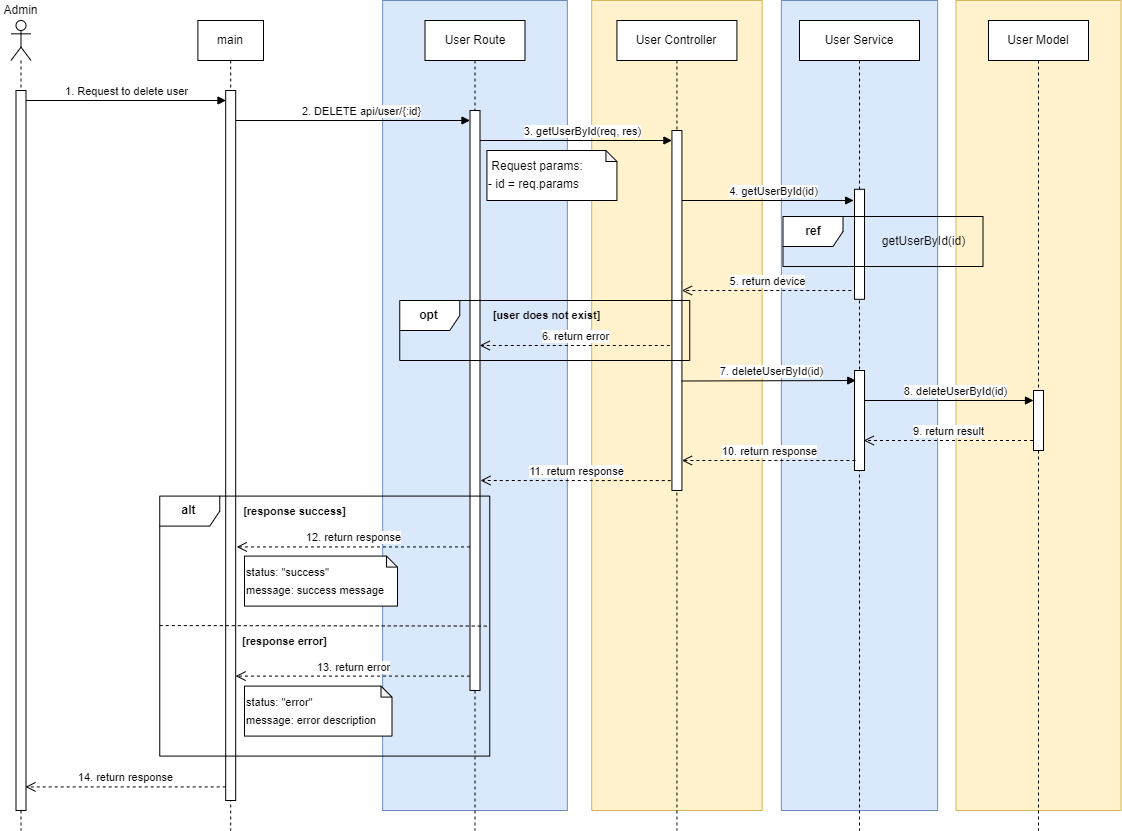
\includegraphics[width=16cm,height=13cm]{Images/sequence_api/deleteUserById.png}
  \caption[Sơ đồ tuần tự cho API xóa thông tin người dùng ]{\bfseries \fontsize{12pt}{0pt}
  \selectfont Sơ đồ tuần tự cho API xóa thông tin người dùng }
  \label{api_deleteUser} %đặt tên cho ảnh
\end{figure}
Hình \ref{api_deleteUser} mô tả quá trình xóa thông tin người dùng trong hệ thống. Người dùng (quản trị viên) gửi yêu cầu xóa thông tin người dùng, thông qua các tầng của hệ thống, 
yêu cầu này được xử lý bởi UserController. UserController gửi truy vấn đến UserService để kiểm tra thông tin người dùng trong hệ thống dựa theo id (ID của người dùng) được truyền vào từ yêu cầu. 
Nếu không tồn tại người dùng, hệ thống sẽ trả về response lỗi tương ứng, ngược lại, UserController tiếp tục gửi truy vấn đến UserService, UserService gửi truy vấn đến UserModel để xóa thông tin
người dùng. Sau đó, kết quả cập nhật được trả về từ UserModel và được gửi trở lại UserRoute để trả về response cho người dùng. Nếu quá trình thực hiện thành công, hệ thống trả về response kết quả cho quản trị viên. Nếu có lỗi xảy ra
 trong quá trình này, hệ thống trả về response lỗi tương ứng.

% \linebreak


% ----------------------------------------------

% ------------------------Chat----------------------


\paragraph{API liên quan đến việc chat}
\mbox{}

% ----------------------------------------------

% -------------------------ECG----------------------------
\paragraph{API liên quan đến bản ghi ECG}
\mbox{}

\begin{figure}[H]
  \centering
  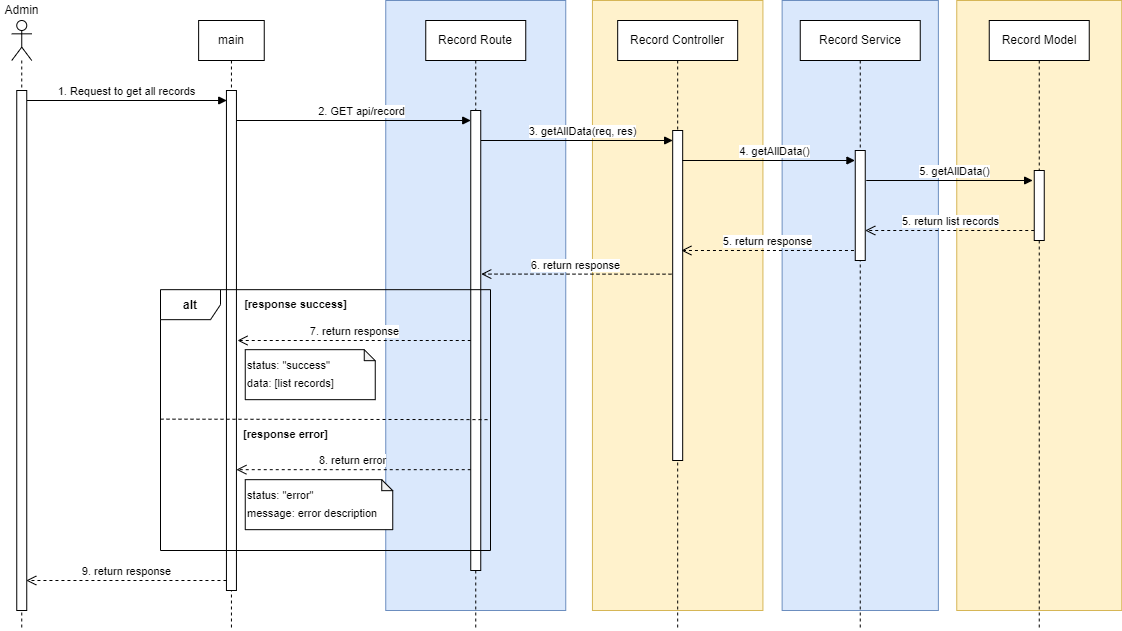
\includegraphics[width=16cm,height=9cm]{Images/sequence_api/getAllRecord.png}
  \caption[Sơ đồ tuần tự cho API lấy danh sách tất cả phiên đo ECG ]{\bfseries \fontsize{12pt}{0pt}
  \selectfont Sơ đồ tuần tự cho API lấy danh sách tất cả phiên đo ECG }
  \label{api_getAllEcgRecords} %đặt tên cho ảnh
\end{figure}
Hình \ref{api_getAllEcgRecords} mô tả quá trình lấy danh sách tất cả phiên đo ECG (Electrocardiogram) của tất cả bệnh nhân trong hệ thống. Người dùng (quản trị viên) gửi yêu cầu lấy danh sách phiên đo ECG của tất cả bệnh nhân, thông qua các tầng của hệ thống, 
yêu cầu này được xử lý bởi RecordController. RecordController tiếp tục gửi truy vấn đến RecordService, RecordService gửi truy vấn đến RecordModel để lấy danh sách dữ liệu ECG. Sau đó, danh sách dữ liệu ECG được trả về từ RecordModel và được gửi trở lại RecordRoute
 để trả về response cho người dùng. Nếu quá trình thực hiện thành công, hệ thống trả về response chứa danh sách bản ghi ECG cho quản trị viên. Nếu có lỗi xảy ra trong quá trình này, hệ thống trả về response lỗi tương ứng. Sau khi xử lý, response cuối cùng được trả về tới người dùng (quản trị viên).

\begin{figure}[H]
  \centering
  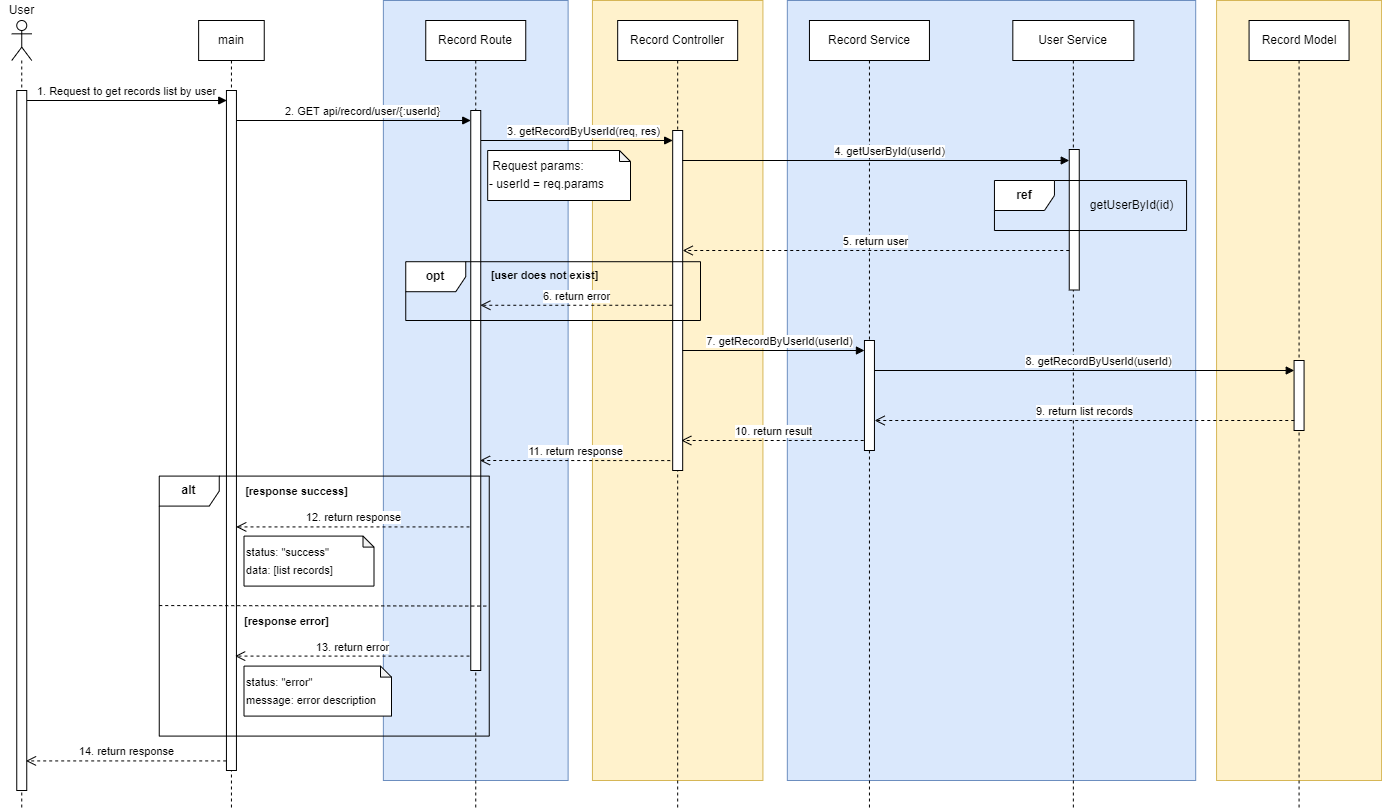
\includegraphics[width=16cm,height=10.5cm]{Images/sequence_api/getRecordsByUser.png}
  \caption[Sơ đồ tuần tự cho API lấy danh sách phiên đo ECG của một bệnh nhân ]{\bfseries \fontsize{12pt}{0pt}
  \selectfont Sơ đồ tuần tự cho API lấy danh sách phiên đo ECG của một bệnh nhân }
  \label{api_getRecordsByUser} %đặt tên cho ảnh
\end{figure}
Hình \ref{api_getRecordsByUser} mô tả quá trình lấy danh sách các phiên đo ECG (Electrocardiogram) của một bệnh nhân trong hệ thống. Người dùng (quản trị viên) gửi yêu cầu lấy danh sách các phiên đo ECG của bệnh nhân, thông qua các tầng của hệ thống, 
yêu cầu này được xử lý bởi RecordController. RecordController gửi truy vấn đến UserService để kiểm tra thông tin bệnh nhân có tồn tại trong hệ thống dựa theo userId (ID của bệnh nhân) được truyền vào từ yêu cầu. Nếu hệ thống không tồn tại bệnh nhân, hệ thống sẽ
trả về response lỗi tương ứng. Nếu bệnh nhân có trong hệ thống, RecordController tiếp tục gửi truy vấn đến RecordService, RecordService gửi truy vấn đến RecordModel để lấy danh sách dữ liệu ECG dựa trên userId (ID của bệnh nhân) được truyền vào từ yêu cầu. 
Sau đó, danh sách dữ liệu ECG được trả về từ RecordModel và được gửi trở lại RecordRoute để trả về response cho người dùng. Nếu quá trình thực hiện thành công, hệ thống trả về response chứa danh sách bản ghi ECG của bệnh nhân cho quản trị viên. Nếu có lỗi xảy ra
 trong quá trình này, hệ thống trả về response lỗi tương ứng. Sau khi xử lý, response cuối cùng được trả về tới người dùng (quản trị viên).

 \begin{figure}[H]
  \centering
  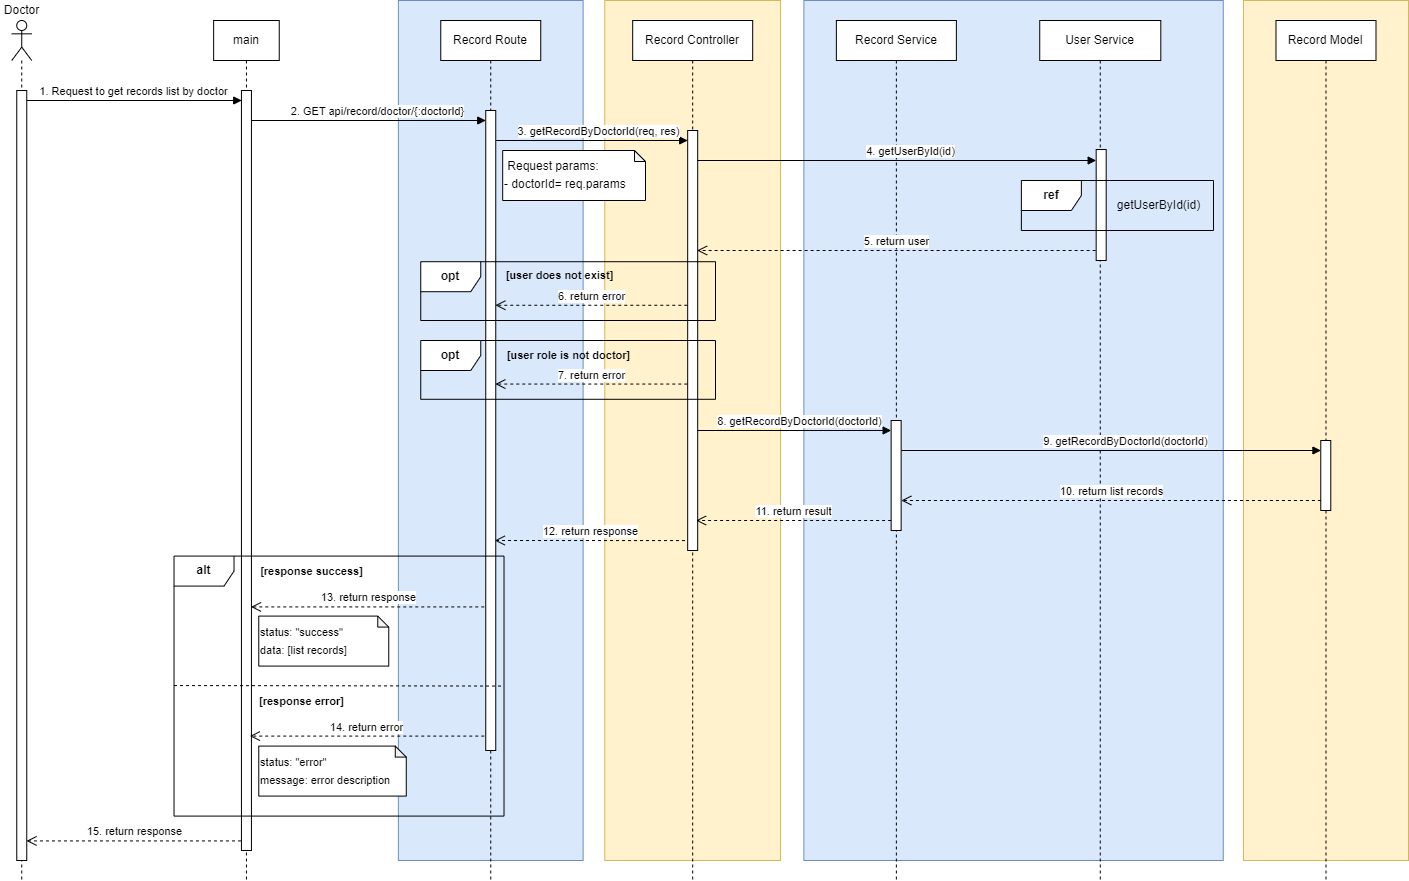
\includegraphics[width=16cm,height=11cm]{Images/sequence_api/getRecordsByDoctor.png}
  \caption[Sơ đồ tuần tự cho API lấy danh sách phiên đo ECG của bệnh nhân được quản lý bởi một bác sỹ ]{\bfseries \fontsize{12pt}{0pt}
  \selectfont Sơ đồ tuần tự cho API lấy danh sách phiên đo ECG của bệnh nhân được quản lý bởi một bác sỹ}
  \label{api_getRecordsByDoctor} %đặt tên cho ảnh
\end{figure}
Hình \ref{api_getRecordsByDoctor} mô tả quá trình lấy danh sách các phiên đo ECG (Electrocardiogram) của bệnh nhân được quản lý bởi một bác sỹ trong hệ thống. Người dùng (quản trị viên) gửi yêu cầu lấy danh sách các phiên đo ECG của bệnh nhân được quản lý bởi một bác sỹ, 
thông qua các tầng của hệ thống, yêu cầu này được xử lý bởi RecordController. RecordController gửi truy vấn đến UserService để kiểm tra thông tin bác sỹ có tồn tại trong hệ thống dựa theo doctorId (ID của bác sỹ) được truyền vào từ yêu cầu. Nếu hệ thống không tồn tại bác sỹ hay không phải là bác sỹ, hệ thống sẽ
trả về response lỗi tương ứng. Nếu bác sỹ có trong hệ thống, RecordController tiếp tục gửi truy vấn đến RecordService, RecordService gửi truy vấn đến RecordModel để lấy danh sách dữ liệu ECG dựa trên doctorId (ID của bác sỹ) được truyền vào từ yêu cầu. 
Sau đó, danh sách dữ liệu ECG được trả về từ RecordModel và được gửi trở lại RecordRoute để trả về response cho người dùng. Nếu quá trình thực hiện thành công, hệ thống trả về response chứa danh sách bản ghi ECG của bệnh nhân cho quản trị viên. Nếu có lỗi xảy ra
 trong quá trình này, hệ thống trả về response lỗi tương ứng. Sau khi xử lý, response cuối cùng được trả về tới người dùng (quản trị viên).

\begin{figure}[H]
  \centering
  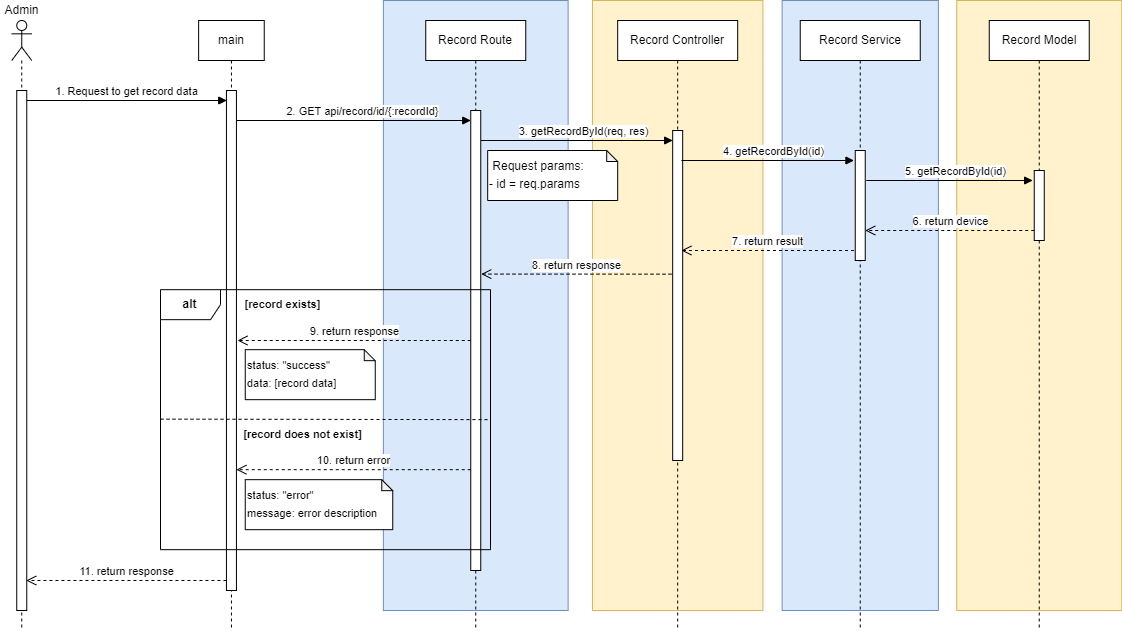
\includegraphics[width=16cm,height=9cm]{Images/sequence_api/getRecordById.png}
  \caption[Sơ đồ tuần tự cho API lấy thông tin một phiên đo ECG ]{\bfseries \fontsize{12pt}{0pt}
  \selectfont Sơ đồ tuần tự cho API lấy thông tin một phiên đo ECG }
  \label{api_getRecordById} %đặt tên cho ảnh
\end{figure}
Hình \ref{api_getRecordById} mô tả quá trình lấy thông tin một phiên đo ECG (Electrocardiogram) của bệnh nhân trong hệ thống. Người dùng (quản trị viên) gửi yêu cầu lấy thông tin một phiên đo ECG của bệnh nhân, thông qua các tầng của hệ thống, 
yêu cầu này được xử lý bởi RecordController. RecordController tiếp tục gửi truy vấn đến RecordService, RecordService gửi truy vấn đến RecordModel để lấy thông tin dữ liệu ECG dựa trên recordId (ID của phiên đo) được truyền vào từ yêu cầu. 
Sau đó, thông tin dữ liệu ECG được trả về từ RecordModel và được gửi trở lại RecordRoute để trả về response cho người dùng. Nếu quá trình thực hiện thành công, hệ thống trả về response chứa danh sách bản ghi ECG cho quản trị viên. Nếu có lỗi xảy ra
 trong quá trình này, hệ thống trả về response lỗi tương ứng. Sau khi xử lý, response cuối cùng được trả về tới người dùng (quản trị viên).

 \begin{figure}[H]
  \centering
  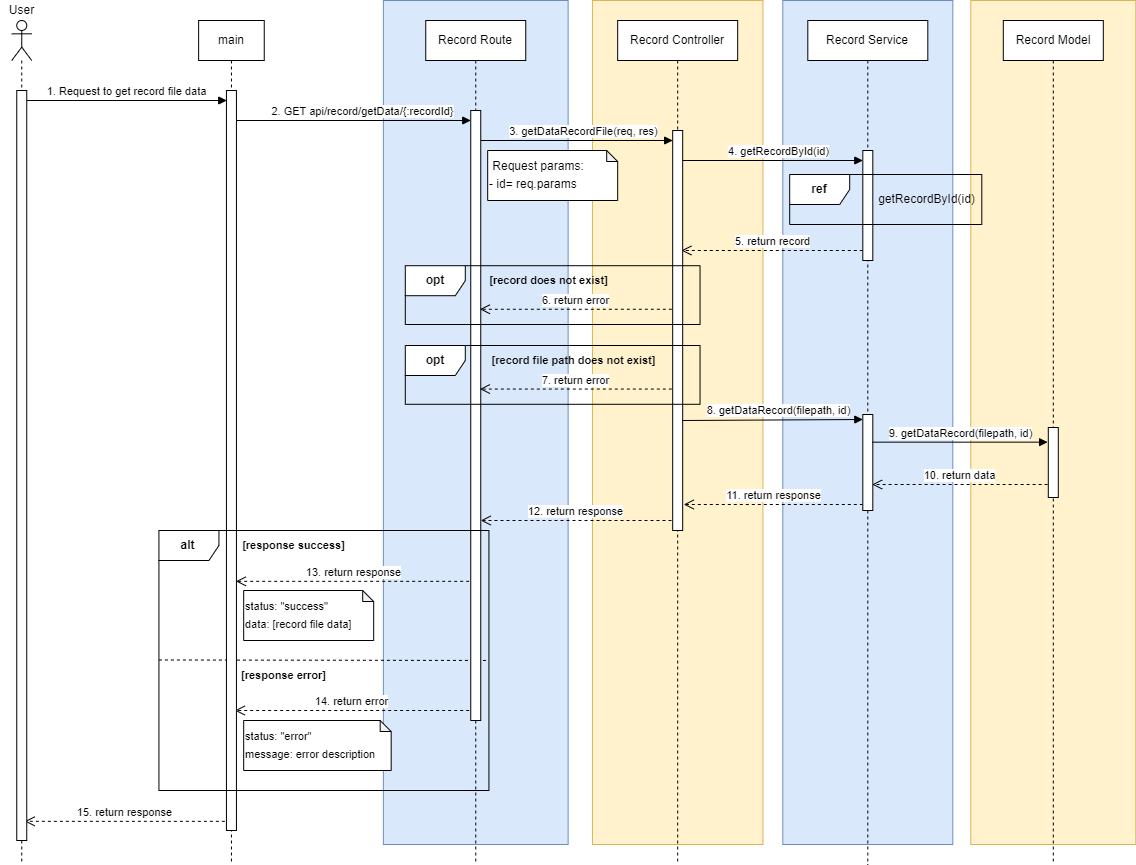
\includegraphics[width=16cm,height=11.5cm]{Images/sequence_api/getRecordDataById.png}
  \caption[Sơ đồ tuần tự cho API lấy dữ liệu một phiên đo ECG ]{\bfseries \fontsize{12pt}{0pt}
  \selectfont Sơ đồ tuần tự cho API lấy dữ liệu một phiên đo ECG }
  \label{api_getRecordDataById} %đặt tên cho ảnh
\end{figure}
Hình \ref{api_getRecordDataById} mô tả quá trình lấy dữ liệu một phiên đo ECG (Electrocardiogram) của bệnh nhân trong hệ thống. Người dùng (quản trị viên) gửi yêu cầu lấy dữ liệu một phiên đo ECG của bệnh nhân, thông qua các tầng của hệ thống, 
yêu cầu này được xử lý bởi RecordController. RecordController gửi truy vấn đến RecordService để kiểm tra thông tin, đường dẫn bản ghi có tồn tại trong hệ thống dựa theo recordId (ID của phiên đo) được truyền vào từ yêu cầu. Nếu hệ thống không tồn tại phiên đo hay đường dẫn bản ghi, hệ thống sẽ
trả về response lỗi tương ứng. Nếu bản ghi có trong hệ thống, RecordController tiếp tục gửi truy vấn đến RecordService, RecordService gửi truy vấn đến RecordModel để lấy dữ liệu ECG dựa trên recordId (ID của phiên đo) được truyền vào từ yêu cầu. 
Sau đó, dữ liệu ECG được trả về từ RecordModel và được gửi trở lại RecordRoute để trả về response cho người dùng. Nếu quá trình thực hiện thành công, hệ thống trả về response chứa danh sách bản ghi ECG cho quản trị viên. Nếu có lỗi xảy ra
 trong quá trình này, hệ thống trả về response lỗi tương ứng. Sau khi xử lý, response cuối cùng được trả về tới người dùng (quản trị viên).


 \begin{figure}[H]
  \centering
  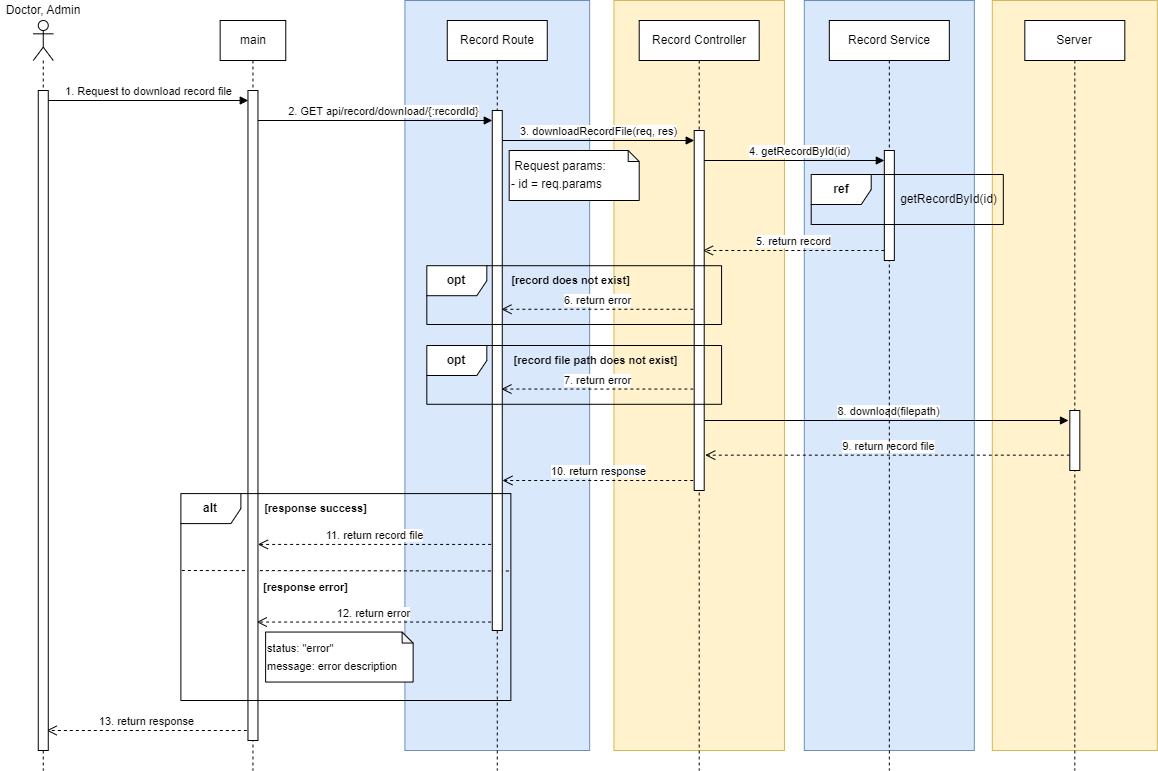
\includegraphics[width=16cm,height=11cm]{Images/sequence_api/downloadRecordDataById.png}
  \caption[Sơ đồ tuần tự cho API tải tệp dữ liệu một phiên đo ECG ]{\bfseries \fontsize{12pt}{0pt}
  \selectfont Sơ đồ tuần tự cho API tải tệp dữ liệu một phiên đo ECG }
  \label{api_downloadRecordDataById} %đặt tên cho ảnh
\end{figure}
Hình \ref{api_downloadRecordDataById} mô tả quá trình tải tệp dữ liệu một phiên đo ECG (Electrocardiogram) của bệnh nhân trong hệ thống. Người dùng (quản trị viên) gửi yêu cầu tải dữ liệu một phiên đo ECG của bệnh nhân, thông qua các tầng của hệ thống, 
yêu cầu này được xử lý bởi RecordController. RecordController gửi truy vấn đến RecordService để kiểm tra thông tin, đường dẫn bản ghi có tồn tại trong hệ thống dựa theo recordId (ID của phiên đo) được truyền vào từ yêu cầu. Nếu hệ thống không tồn tại phiên đo hay đường dẫn bản ghi, hệ thống sẽ
trả về response lỗi tương ứng. Nếu bản ghi có trong hệ thống, RecordController tiếp tục gửi truy vấn đến RecordService, RecordService gửi truy vấn đến Server để lấy tệp dữ liệu ECG dựa trên đường dẫn tệp bản ghi được truyền vào từ yêu cầu. 
Sau đó, tệp bản ghi ECG được trả về từ Server và được gửi trở lại RecordRoute để trả về response cho người dùng. Nếu quá trình thực hiện thành công, hệ thống trả về response chứa tệp bản ghi ECG cho quản trị viên. Nếu có lỗi xảy ra
 trong quá trình này, hệ thống trả về response lỗi tương ứng. Sau khi xử lý, response cuối cùng được trả về tới người dùng (quản trị viên).

 \begin{figure}[H]
  \centering
  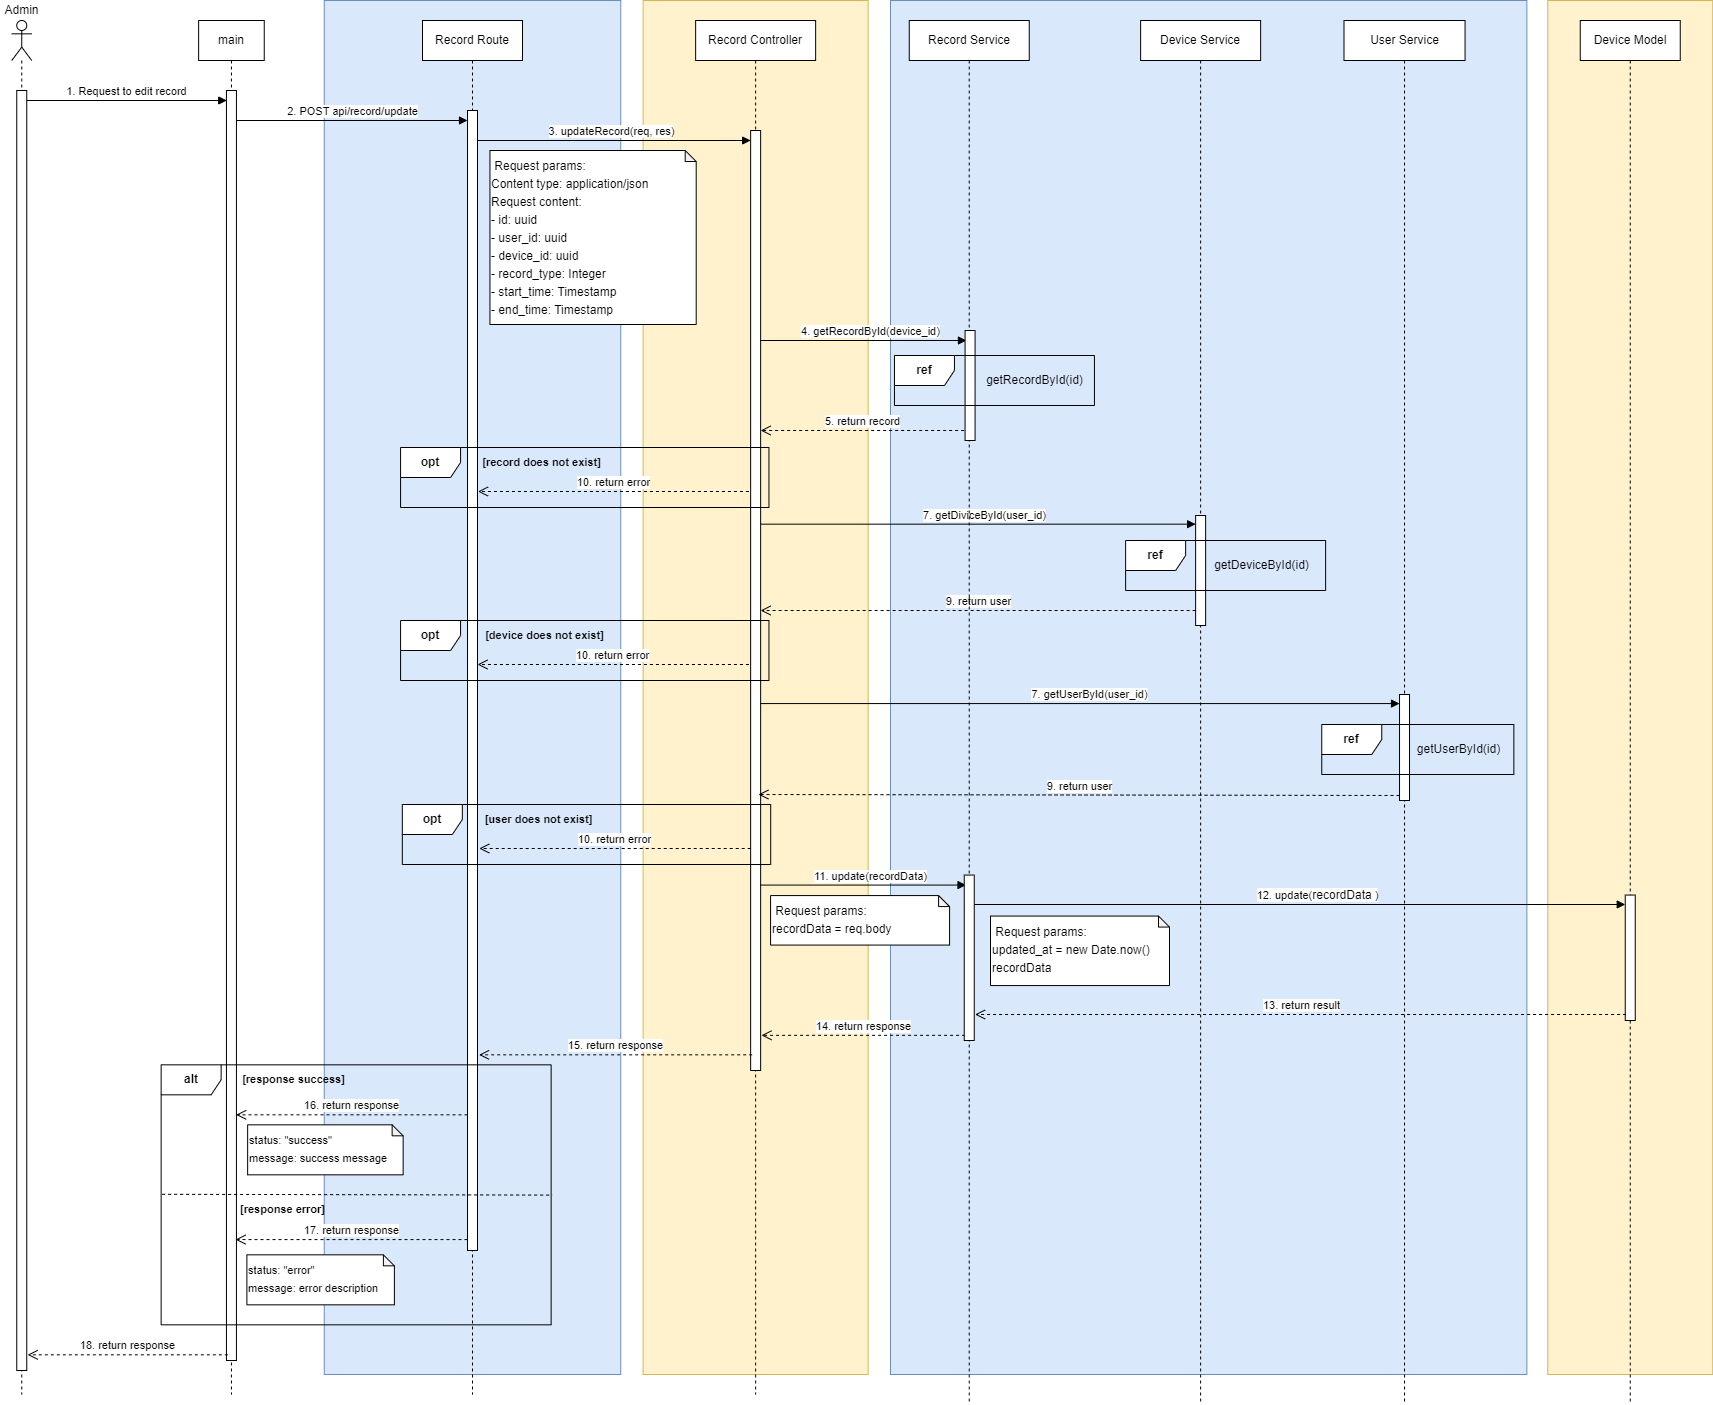
\includegraphics[width=16cm,height=14cm]{Images/sequence_api/editRecordById.png}
  \caption[Sơ đồ tuần tự cho API cập nhật thông tin một phiên đo ECG ]{\bfseries \fontsize{12pt}{0pt}
  \selectfont Sơ đồ tuần tự cho API cập nhật thông tin một phiên đo ECG }
  \label{api_editRecordById} %đặt tên cho ảnh
\end{figure}
Hình \ref{api_editRecordById} mô tả quá trình cập nhật thông tin một phiên đo ECG (Electrocardiogram) của bệnh nhân trong hệ thống. Người dùng (quản trị viên) gửi yêu cầu cập nhật thông tin một phiên đo ECG của bệnh nhân, thông qua các tầng của hệ thống, 
yêu cầu này được xử lý bởi RecordController. RecordController gửi truy vấn đến RecordService, DeviceService, UserService để kiểm tra thông tin bản ghi, thiết bị và bệnh nhân trong hệ thống dựa theo id (ID của phiên đo), user\_id (ID của bệnh nhân), device\_id (ID của thiết bị)
 được truyền vào từ yêu cầu. Nếu hệ thống không tồn tại phiên đo, bệnh nhân hay thiết bị, hệ thống sẽ trả về response lỗi tương ứng. Nếu thông tin có trong hệ thống, RecordController tiếp tục gửi truy vấn đến RecordService, RecordService gửi truy vấn đến RecordModel để cập nhật thông tin
phiên đo ECG dựa trên thông tin được truyền vào từ yêu cầu. Sau đó, kết quả cập nhật được trả về từ RecordModel và được gửi trở lại RecordRoute để trả về response cho người dùng. Nếu quá trình thực hiện thành công, hệ thống trả về response kết quả cho quản trị viên. Nếu có lỗi xảy ra
 trong quá trình này, hệ thống trả về response lỗi tương ứng. Sau khi xử lý, response cuối cùng được trả về tới người dùng (quản trị viên).

 \begin{figure}[H]
  \centering
  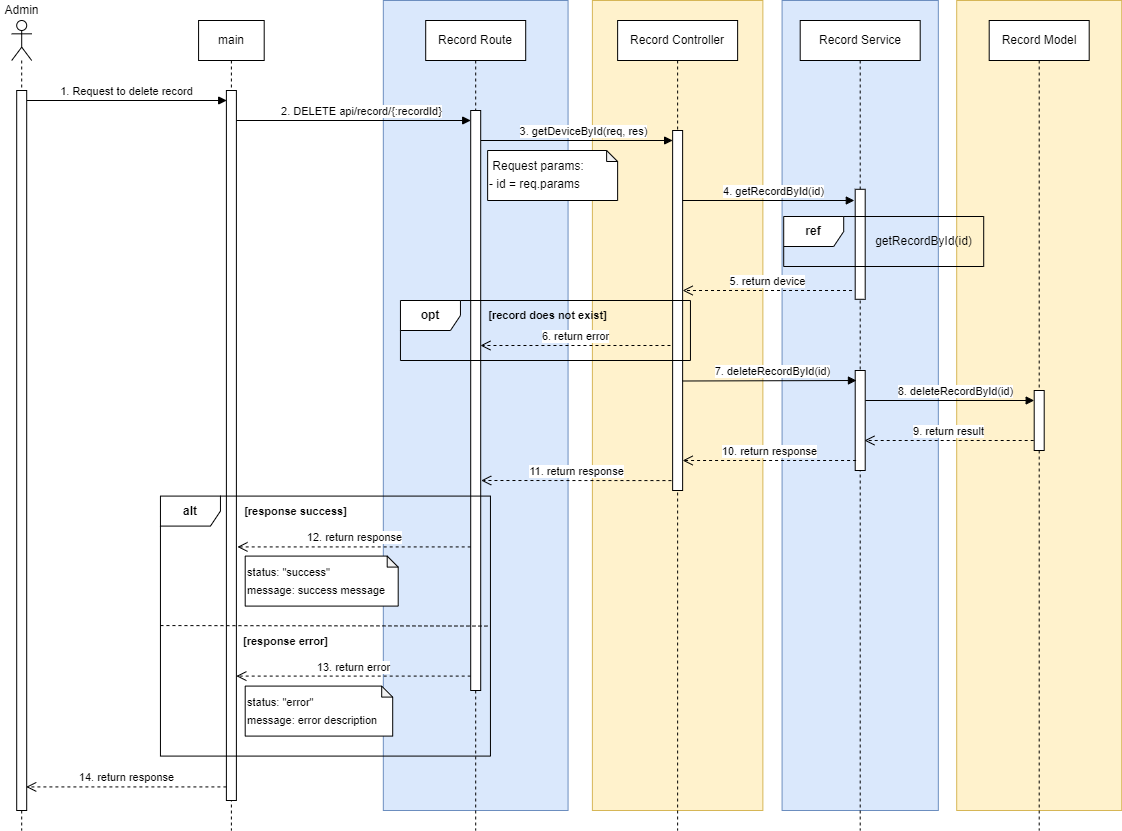
\includegraphics[width=16cm,height=11.5cm]{Images/sequence_api/deleteRecordById.png}
  \caption[Sơ đồ tuần tự cho API xóa thông tin một phiên đo ECG ]{\bfseries \fontsize{12pt}{0pt}
  \selectfont Sơ đồ tuần tự cho API xóa thông tin một phiên đo ECG }
  \label{api_deleteRecordById} %đặt tên cho ảnh
\end{figure}
Hình \ref{api_deleteRecordById} mô tả quá trình xóa thông tin một phiên đo ECG (Electrocardiogram) của bệnh nhân trong hệ thống. Người dùng (quản trị viên) gửi yêu cầu xóa thông tin một phiên đo ECG của bệnh nhân, thông qua các tầng của hệ thống, 
yêu cầu này được xử lý bởi RecordController. RecordController gửi truy vấn đến RecordService để kiểm tra thông tin bản ghi trong hệ thống dựa theo recordId (ID của phiên đo) được truyền vào từ yêu cầu. Nếu hệ thống không tồn tại phiên đo, hệ thống sẽ trả về response lỗi tương ứng. 
Nếu thông tin phiên đo có trong hệ thống, RecordController tiếp tục gửi truy vấn đến RecordService, RecordService gửi truy vấn đến RecordModel để xóa thông tin phiên đo ECG dựa trên recordId (ID của phiên đo) được truyền vào từ yêu cầu. Sau đó, kết quả cập nhật được trả về từ RecordModel 
và được gửi trở lại RecordRoute để trả về response cho người dùng. Nếu quá trình thực hiện thành công, hệ thống trả về response kết quả cho quản trị viên. Nếu có lỗi xảy ra  trong quá trình này, hệ thống trả về response lỗi tương ứng. Sau khi xử lý, response cuối cùng được trả về tới người dùng (quản trị viên).


% -----------------------------------------------------

% -------------------------Device----------------------------
\paragraph{API liên quan đến thiết bị}
\mbox{}

\begin{figure}[H]
  \centering
  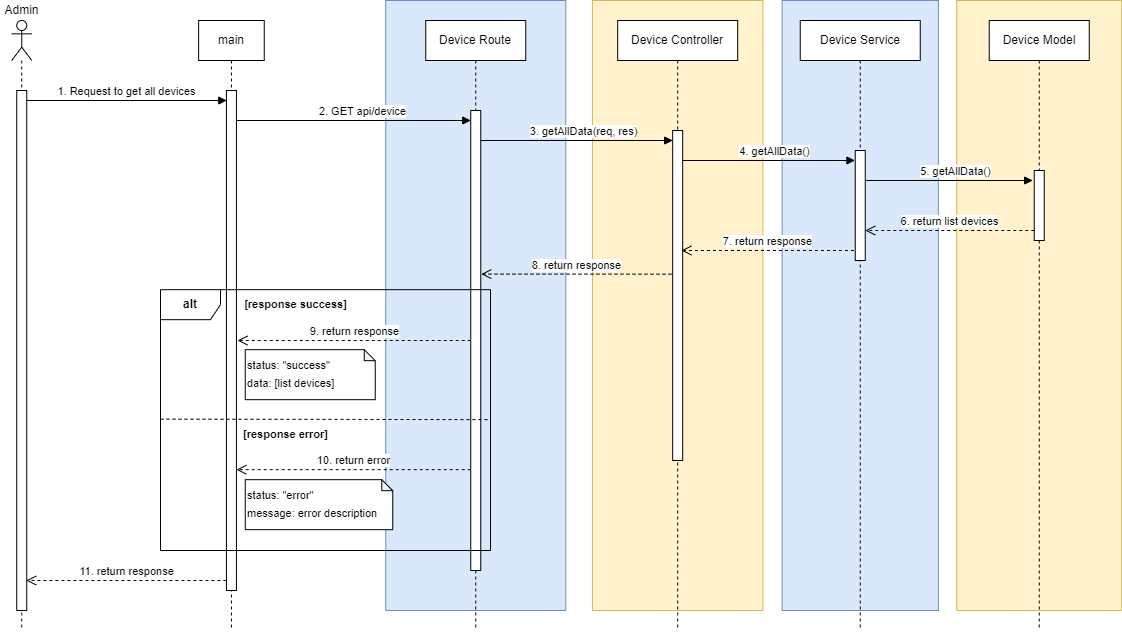
\includegraphics[width=16cm,height=9cm]{Images/sequence_api/getAllDevices.png}
  \caption[Sơ đồ tuần tự cho API lấy danh sách tất cả thiết bị ]{\bfseries \fontsize{12pt}{0pt}
  \selectfont Sơ đồ tuần tự cho API lấy danh sách tất cả thiết bị }
  \label{api_getAllDevices} %đặt tên cho ảnh
\end{figure}
Hình \ref{api_getAllDevices} mô tả quá trình lấy danh sách tất cả thiết bị trong hệ thống. Người dùng (quản trị viên) gửi yêu cầu lấy danh sách thiết bị, thông qua các tầng của hệ thống, 
yêu cầu này được xử lý bởi DeviceController. DeviceController tiếp tục gửi truy vấn đến DeviceService, DeviceService gửi truy vấn đến DeviceModel để lấy danh sách thiết bị. Sau đó, danh sách thiết bị được trả về từ DeviceModel và được gửi trở lại DeviceRoute
 để trả về response cho người dùng. Nếu quá trình thực hiện thành công, hệ thống trả về response chứa danh sách thiết bị cho quản trị viên. Nếu có lỗi xảy ra trong quá trình này, hệ thống trả về response lỗi tương ứng. Sau khi xử lý, response cuối cùng được 
trả về tới người dùng (quản trị viên).

\begin{figure}[H]
  \centering
  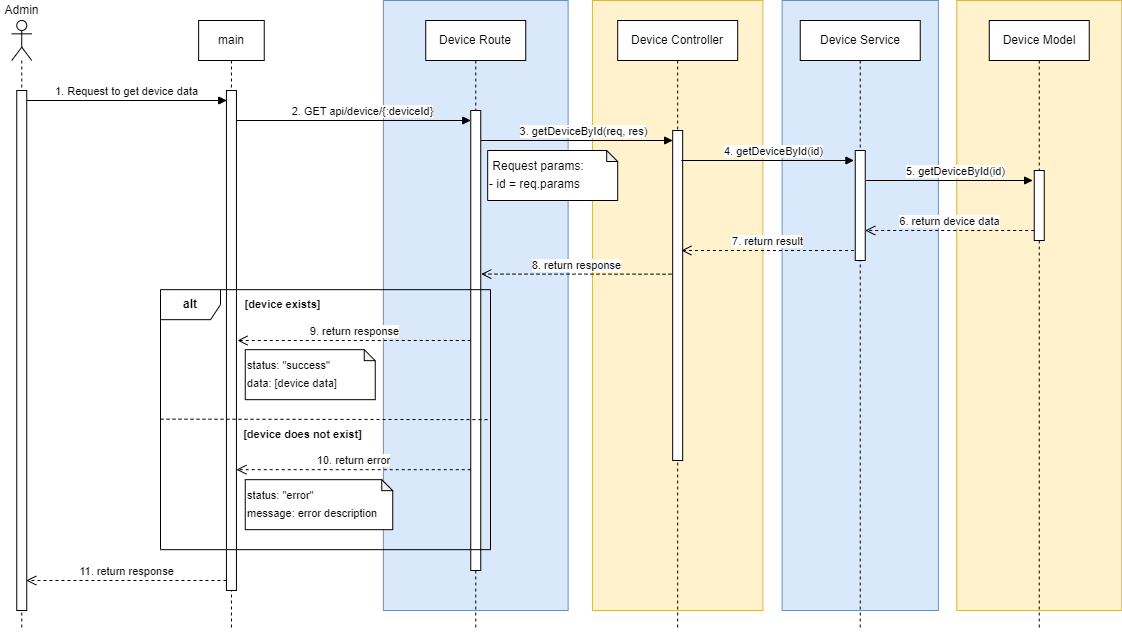
\includegraphics[width=16cm,height=10cm]{Images/sequence_api/getDeviceById.png}
  \caption[Sơ đồ tuần tự cho API lấy thông tin thiết bị dựa trên ID]{\bfseries \fontsize{12pt}{0pt}
  \selectfont Sơ đồ tuần tự cho API lấy thông tin thiết bị dựa trên ID }
  \label{api_getDeviceById} %đặt tên cho ảnh
\end{figure}
Hình \ref{api_getDeviceById} mô tả quá trình lấy thông tin thiết bị dựa trên ID trong hệ thống. Người dùng (quản trị viên) gửi yêu cầu lấy thông tin thiết bị theo ID, thông qua các tầng của hệ thống, 
yêu cầu này được xử lý bởi DeviceController. DeviceController tiếp tục gửi truy vấn đến DeviceService, DeviceService gửi truy vấn đến DeviceModel để lấy thông tin thiết bị dựa theo deviceId (ID của thiết bị). 
Sau đó, thông tin thiết bị được trả về từ DeviceModel và được gửi trở lại DeviceRoute để trả về response cho người dùng. Nếu thiết bị tồn tại, hệ thống trả về response chứa thông tin thiết bị cho quản trị viên. Nếu có lỗi xảy ra trong quá trình này, hệ thống trả về response lỗi tương ứng. 
Sau khi xử lý, response cuối cùng được trả về tới người dùng (quản trị viên).

\begin{figure}[H]
  \centering
  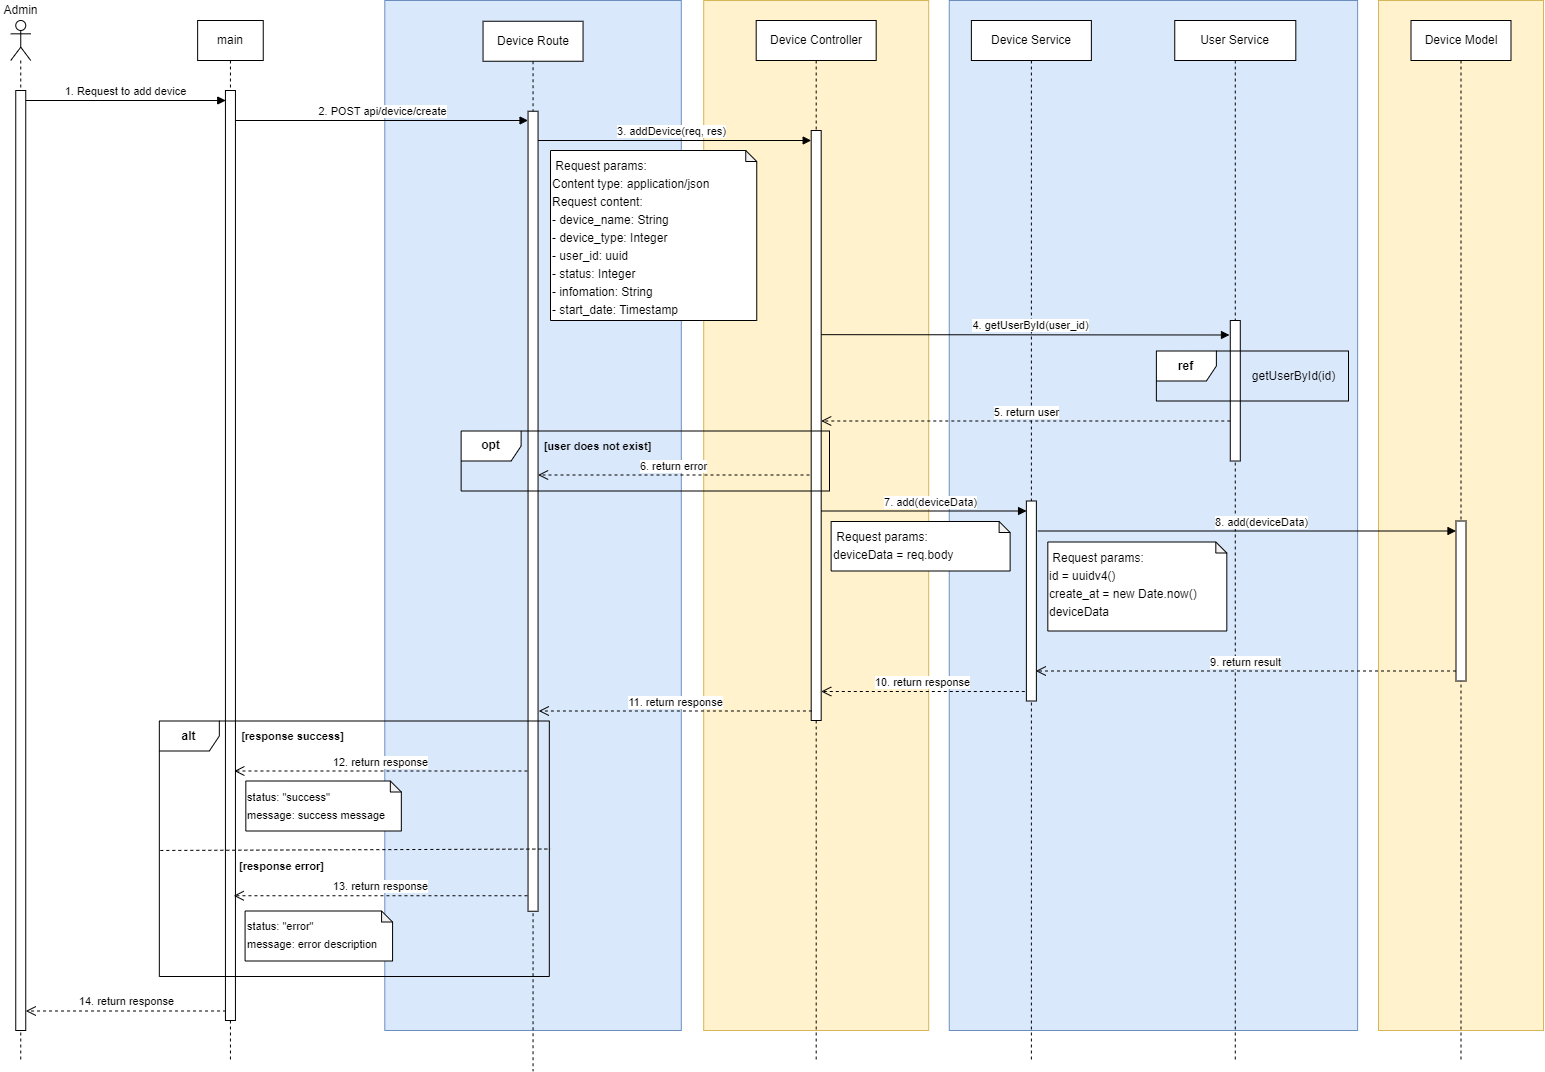
\includegraphics[width=16cm,height=13cm]{Images/sequence_api/addDevice.png}
  \caption[Sơ đồ tuần tự cho API thêm thiết bị]{\bfseries \fontsize{12pt}{0pt}
  \selectfont Sơ đồ tuần tự cho API thêm thiết bị }
  \label{api_addDevice} %đặt tên cho ảnh
\end{figure}
Hình \ref{api_addDevice} mô tả quá trình thêm thiết bị vào hệ thống. Người dùng (quản trị viên) gửi yêu cầu tạo thông tin thiết bị, thông qua các tầng của hệ thống, 
yêu cầu này được xử lý bởi DeviceController. DeviceController gửi truy vấn đến UserService để kiểm tra thông tin người dùng trong hệ thống dựa theo user\_id (ID của bệnh nhân) được truyền vào từ yêu cầu. 
Nếu hệ thống không tồn tại bệnh nhân, hệ thống sẽ trả về response lỗi tương ứng. Nếu thông tin có trong hệ thống, DeviceController tiếp tục gửi truy vấn đến DeviceService, DeviceService gửi truy vấn đến DeviceModel để thêm thông tin thiết bị 
dựa theo thông tin truyền vào. Sau đó, kết quả tạo được trả về từ DeviceModel và được gửi trở lại DeviceRoute để trả về response cho người dùng. Nếu kết quả tạo thành công, hệ thống trả về response chứa thông tin thiết bị cho quản trị viên. 
Nếu có lỗi xảy ra trong quá trình này, hệ thống trả về response lỗi tương ứng. Sau khi xử lý, response cuối cùng được trả về tới người dùng (quản trị viên).

\begin{figure}[H]
  \centering
  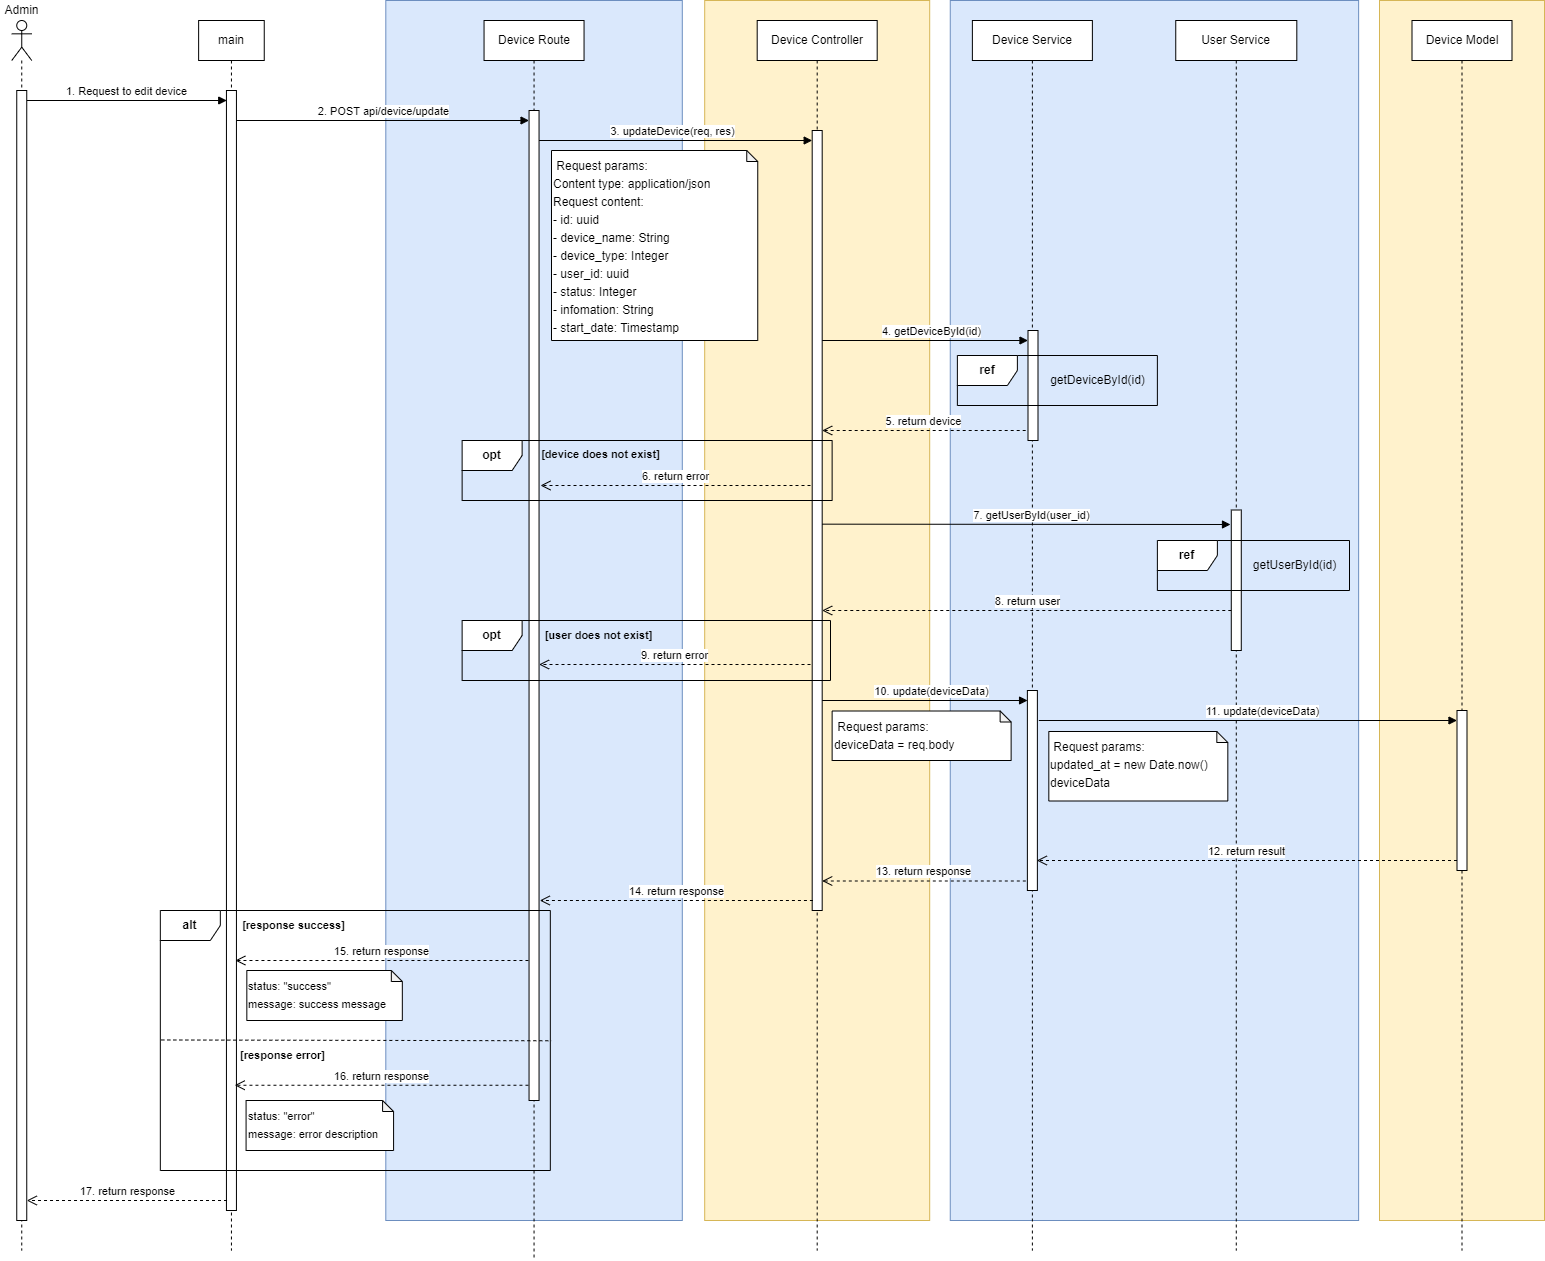
\includegraphics[width=16cm,height=14cm]{Images/sequence_api/editDevice.png}
  \caption[Sơ đồ tuần tự cho API cập nhật thông tin thiết bị ]{\bfseries \fontsize{12pt}{0pt}
  \selectfont Sơ đồ tuần tự cho API cập nhật thông tin thiết bị }
  \label{api_editDevice} %đặt tên cho ảnh
\end{figure}
Hình \ref{api_editDevice} mô tả quá trình cập nhật thông tin một thiết bị trong hệ thống. Người dùng (quản trị viên) gửi yêu cầu cập nhật thông tin một thiết bị, thông qua các tầng của hệ thống, 
yêu cầu này được xử lý bởi DeviceController. DeviceController gửi truy vấn đến DeviceService, UserService để kiểm tra thông tin thiết bị và bệnh nhân trong hệ thống dựa theo id (ID của thiết bị),
 user\_id (ID của bệnh nhân) được truyền vào từ yêu cầu. Nếu hệ thống không tồn tại thông tin, hệ thống sẽ trả về response lỗi tương ứng. Ngược lại, DeviceController tiếp tục gửi truy vấn đến DeviceService, 
 DeviceService gửi truy vấn đến DeviceModel để cập nhật thông tin thiết bị dựa trên thông tin được truyền vào từ yêu cầu. Sau đó, kết quả cập nhật được trả về từ DeviceModel và được gửi trở lại DeviceRoute để 
 trả về response cho người dùng. Nếu quá trình thực hiện thành công, hệ thống trả về response kết quả cho quản trị viên. Nếu có lỗi xảy ra trong quá trình này, hệ thống trả về response lỗi tương ứng. Sau khi xử lý, response cuối cùng được trả về tới người dùng (quản trị viên).

 \begin{figure}[H]
  \centering
  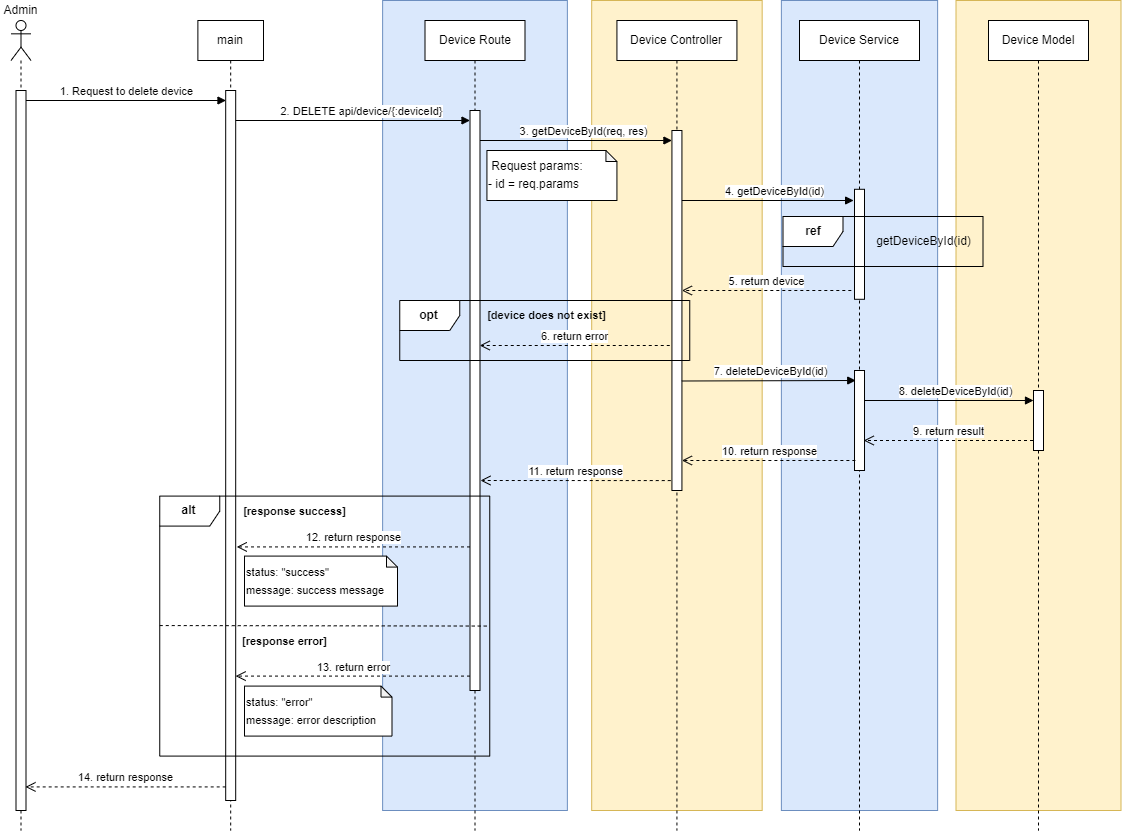
\includegraphics[width=16cm,height=12cm]{Images/sequence_api/deleteDeviceById.png}
  \caption[Sơ đồ tuần tự cho API xóa thiết bị]{\bfseries \fontsize{12pt}{0pt}
  \selectfont Sơ đồ tuần tự cho API xóa thiết bị }
  \label{api_deleteDeviceById} %đặt tên cho ảnh
\end{figure}
Hình \ref{api_deleteDeviceById} mô tả quá trình xóa thiết bị trong hệ thống. Người dùng (quản trị viên) gửi yêu cầu xóa thông tin thiết bị, thông qua các tầng của hệ thống, 
yêu cầu này được xử lý bởi DeviceController. DeviceController gửi truy vấn đến DeviceService để kiểm tra thông tin thiết bị trong hệ thống dựa theo deviceId (ID của thiết bị) được truyền vào từ yêu cầu. 
Nếu hệ thống không tồn tại thiết bị, hệ thống sẽ trả về response lỗi tương ứng. Nếu thông tin có trong hệ thống, DeviceController tiếp tục gửi truy vấn đến DeviceService, DeviceService gửi truy vấn đến DeviceModel để xóa thông tin thiết bị 
dựa theo thông tin truyền vào. Sau đó, kết quả tạo được trả về từ DeviceModel và được gửi trở lại DeviceRoute để trả về response cho người dùng. Nếu kết quả xóa thành công, hệ thống trả về response chứa kết quả cho quản trị viên. 
Nếu có lỗi xảy ra trong quá trình này, hệ thống trả về response lỗi tương ứng. Sau khi xử lý, response cuối cùng được trả về tới người dùng (quản trị viên).

% -----------------------------------------------------

% -----------------------PatientDoctor------------------------------

\paragraph{API liên quan liên quan đến việc phân công bệnh nhân cho bác sỹ}
\mbox{}


\begin{figure}[H]
  \centering
  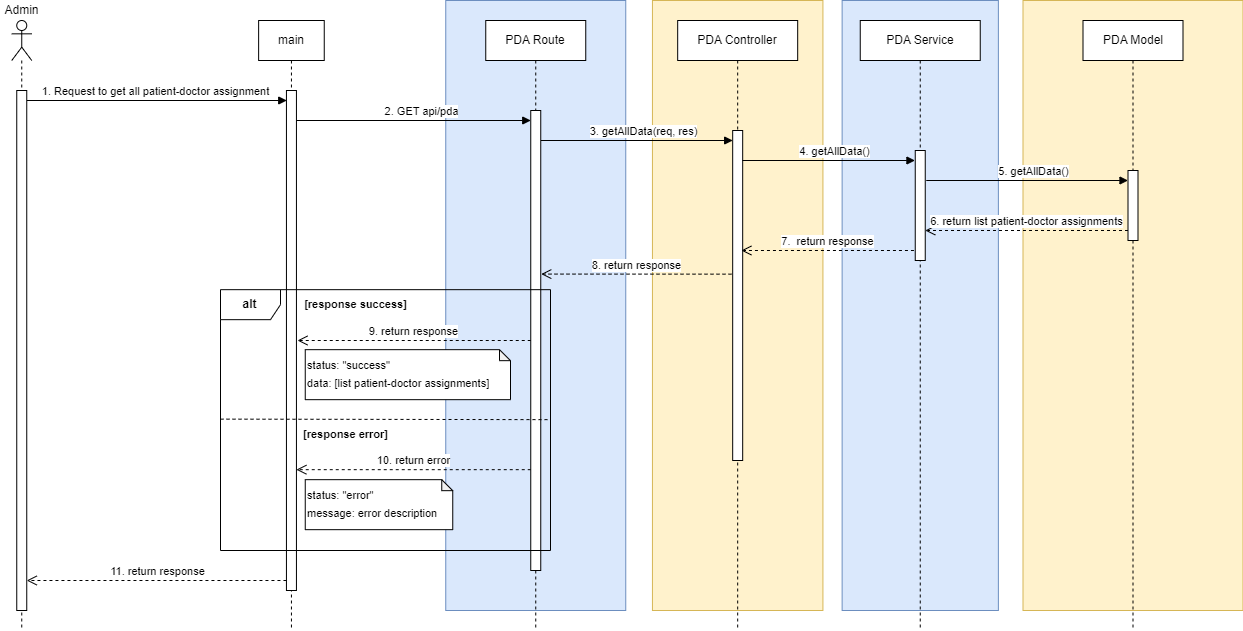
\includegraphics[width=16cm,height=9cm]{Images/sequence_api/getAllPDA.png}
  \caption[Sơ đồ tuần tự cho API lấy danh sách tất cả phân công bác sĩ - bệnh nhân ]{\bfseries \fontsize{12pt}{0pt}
  \selectfont Sơ đồ tuần tự cho API lấy danh sách tất cả phân công bác sĩ - bệnh nhân }
  \label{api_getAllPDA} %đặt tên cho ảnh
\end{figure}
Hình \ref{api_getAllPDA} mô tả quá trình lấy danh sách tất cả phân công bác sĩ - bệnh nhân trong hệ thống. Người dùng (quản trị viên) gửi yêu cầu lấy danh sách phân công bác sĩ - bệnh nhân, thông qua các tầng của hệ thống, 
yêu cầu này được xử lý bởi PDAController. PDAController tiếp tục gửi truy vấn đến PDAService, PDAService gửi truy vấn đến PDAModel để lấy danh sách phân công. Sau đó, danh sách phân công được trả về từ PDAModel và được gửi trở lại PDARoute
 để trả về response cho người dùng. Nếu quá trình thực hiện thành công, hệ thống trả về response chứa danh sách phân công cho quản trị viên. Nếu có lỗi xảy ra trong quá trình này, hệ thống trả về response lỗi tương ứng. Sau khi xử lý, response cuối cùng được 
trả về tới người dùng (quản trị viên).

\begin{figure}[H]
  \centering
  \includegraphics[width=16cm,height=14cm]{Images/sequence_api/addAssignment.png}
  \caption[Sơ đồ tuần tự cho API thêm phân công bệnh nhân - bác sĩ]{\bfseries \fontsize{12pt}{0pt}
  \selectfont Sơ đồ tuần tự cho API thêm phân công bệnh nhân - bác sĩ }
  \label{api_addPDA} %đặt tên cho ảnh
\end{figure}
Hình \ref{api_addPDA} mô tả quá trình thêm phân công bệnh nhân - bác sĩ vào hệ thống. Người dùng (quản trị viên) gửi yêu cầu tạo phân công bệnh nhân - bác sĩ, thông qua các tầng của hệ thống, 
yêu cầu này được xử lý bởi PDAController. PDAController gửi truy vấn đến UserService để kiểm tra thông tin bệnh nhân, bác sĩ trong hệ thống dựa theo patient\_id (ID của bệnh nhân), doctor\_id (ID bác sĩ);PDAService để kiểm
tra bệnh nhân đã có phân công bác sĩ dựa theo patient\_id được truyền vào từ yêu cầu. Nếu hệ thống không tồn tại bệnh nhân, bác sĩ hay bệnh nhân đã có bác sĩ phân công, hệ thống sẽ trả về response lỗi tương ứng. 
Ngược lại, PDAController tiếp tục gửi truy vấn đến PDAService, PDAService gửi truy vấn đến PDAModel để thêm thông tin phân công dựa theo thông tin truyền vào. Sau đó, kết quả tạo được trả về từ PDAModel và được gửi trở lại 
PDARoute để trả về response cho người dùng. Nếu kết quả tạo thành công, hệ thống trả về response chứa kết quả thêm phân công cho quản trị viên. 
Nếu có lỗi xảy ra trong quá trình này, hệ thống trả về response lỗi tương ứng. Sau khi xử lý, response cuối cùng được trả về tới người dùng (quản trị viên).

\begin{figure}[H]
  \centering
  \includegraphics[width=16cm,height=13cm]{Images/sequence_api/editAssignment.png}
  \caption[Sơ đồ tuần tự cho API cập nhật thông tin phân công bệnh nhân - bác sĩ]{\bfseries \fontsize{12pt}{0pt}
  \selectfont Sơ đồ tuần tự cho API cập nhật thông tin phân công bệnh nhân - bác sĩ }
  \label{api_editPDA} %đặt tên cho ảnh
\end{figure}
Hình \ref{api_editPDA} mô tả quá trình cập nhật thông tin phân công bệnh nhân - bác sĩ vào hệ thống. Người dùng (quản trị viên) gửi yêu cầu sửa thông tin phân công bệnh nhân - bác sĩ, thông qua các tầng của hệ thống, 
yêu cầu này được xử lý bởi PDAController. PDAController gửi truy vấn đến UserService để kiểm tra thông tin bệnh nhân, bác sĩ trong hệ thống dựa theo patient\_id (ID của bệnh nhân), doctor\_id (ID bác sĩ);PDAService để kiểm
tra bệnh nhân đã có phân công bác sĩ dựa theo patient\_id được truyền vào từ yêu cầu. Nếu hệ thống không tồn tại bệnh nhân, bác sĩ hay bệnh nhân chưa có bác sĩ phân công, hệ thống sẽ trả về response lỗi tương ứng. 
Ngược lại, PDAController tiếp tục gửi truy vấn đến PDAService, PDAService gửi truy vấn đến PDAModel để sửa thông tin phân công dựa theo thông tin truyền vào. Sau đó, kết quả cập nhật được trả về từ PDAModel và được gửi trở lại 
PDARoute để trả về response cho người dùng. Nếu kết quả tạo thành công, hệ thống trả về response chứa kết quả thêm phân công cho quản trị viên. 
Nếu có lỗi xảy ra trong quá trình này, hệ thống trả về response lỗi tương ứng. Sau khi xử lý, response cuối cùng được trả về tới người dùng (quản trị viên).

\begin{figure}[H]
  \centering
  \includegraphics[width=16cm,height=11cm]{Images/sequence_api/deleteAssignment.png}
  \caption[Sơ đồ tuần tự cho API xóa phân công bệnh nhân - bác sĩ]{\bfseries \fontsize{12pt}{0pt}
  \selectfont Sơ đồ tuần tự cho API xóa phân công bệnh nhân - bác sĩ }
  \label{api_deletePDA} %đặt tên cho ảnh
\end{figure}
Hình \ref{api_deletePDA} mô tả quá trình xóa phân công bệnh nhân - bác sĩ trong hệ thống. Người dùng (quản trị viên) gửi yêu cầu xóa thông tin phân công, thông qua các tầng của hệ thống, 
yêu cầu này được xử lý bởi PDAController. PDAController gửi truy vấn đến PDAService để kiểm tra thông tin phân công trong hệ thống dựa theo pdaId (ID của phân công) được truyền vào từ yêu cầu. 
Nếu hệ thống không tồn tại phân công, hệ thống sẽ trả về response lỗi tương ứng. Nếu thông tin có trong hệ thống, PDAController tiếp tục gửi truy vấn đến PDAService, PDAService gửi truy vấn đến PDAModel để xóa thông tin phân công 
dựa theo thông tin truyền vào. Sau đó, kết quả tạo được trả về từ PDAModel và được gửi trở lại PDARoute để trả về response cho người dùng. Nếu kết quả xóa thành công, hệ thống trả về response chứa kết quả cho quản trị viên. 
% -----------------------------------------------------


\subsection{Kết luận chương}

Chương 3 đã trình bày quá trình thiết kế hệ thống 
dưới góc độ kiến trúc và các thành
 phần cụ thể. Trong quá trình thiết kế, chúng em đã tập trung
  vào việc xây dựng một kiến trúc hoạt động mượt mà và hiệu quả,
   đảm bảo tính bảo mật, hiệu suất và khả năng mở rộng của hệ
    thống.

\newpage